%======================================================================
% MANUAL DE USUARIO - SANDRA DESKTOP CONTAINER (SDC)
% Plataforma de Orquestación Segura para Aplicaciones Distribuidas
% 
% Autor: Carlos Peña
% Empresa: Code Epic Technologies
% Ubicación: Caracas, Venezuela
% Versión: 2026.1 - Stable Build
% Fecha: Marzo 2026
%======================================================================

\documentclass[
    11pt,
    oneside,
    openright,
    spanish,
    a4paper
]{book}

%--------------------------------------------------------------------
% PAQUETES BASE
%--------------------------------------------------------------------
\usepackage{iftex}
\ifPDFTeX
    \usepackage[utf8]{inputenc}
    \usepackage[T1]{fontenc}
    \usepackage{mathpazo}
\else
    \usepackage{fontspec}
\fi

\usepackage[
    margin=2.5cm,
    top=2.5cm,
    bottom=2.5cm,
    left=2.5cm,
    right=2.5cm
]{geometry}

\usepackage{graphicx}
\usepackage{fontawesome5}
\usepackage{wrapfig}
\usepackage{fancyhdr}
\usepackage{emptypage}
\usepackage{titlesec}
\usepackage{titletoc}
\usepackage{makeidx}
\usepackage{setspace}
\usepackage{multicol}
\usepackage{longtable}
\usepackage{array}
\usepackage{booktabs}
\usepackage{caption}
\usepackage{subcaption}
\usepackage{enumitem}
\usepackage{float}
\usepackage{listings}
\usepackage{xcolor}
\usepackage{colortbl}
\usepackage{lettrine}
\usepackage{microtype}
\usepackage{eso-pic}
\usepackage{tikz}
\usetikzlibrary{calc, shapes.geometric, backgrounds, shadows.blur, positioning, arrows.meta}

%--------------------------------------------------------------------
% CONFIGURACION DE COLORES - SANDRA TEAL SOFT
%--------------------------------------------------------------------
\definecolor{sandraDark}{HTML}{2D5A4A}
\definecolor{sandraGreen}{HTML}{4CAF93}
\definecolor{sandraLight}{HTML}{B2E0D0}
\definecolor{sandraAccent}{HTML}{FFC107}
\definecolor{sandraSoft}{HTML}{F5FAF8}
\definecolor{sandraGray}{HTML}{616161}
\definecolor{textDark}{HTML}{263238}
\definecolor{textLight}{HTML}{78909C}
\definecolor{primary}{HTML}{455A64}
\definecolor{secondary}{HTML}{90A4AE}
\definecolor{accent}{HTML}{66BB6A}

%--------------------------------------------------------------------
% CONFIGURACION DE FUENTES
%--------------------------------------------------------------------
\ifPDFTeX
    % Usar fuentes del sistema para PDFTeX
\else
    \setmainfont{Helvetica Neue}[
        UprightFont = *,
        BoldFont = * Bold,
        ItalicFont = * Italic,
        BoldItalicFont = * Bold Italic
    ]
\fi

%--------------------------------------------------------------------
% HYPERREF CON METADATA
%--------------------------------------------------------------------
\usepackage[
    spanish,
    bookmarks=true,
    colorlinks=true,
    linkcolor=sandraDark,
    citecolor=sandraDark,
    urlcolor=sandraGreen,
    pdftitle={Manual de Usuario - Sandra Desktop Container},
    pdfauthor={Carlos Peña},
    pdfsubject={Plataforma de Orquestación Segura para Aplicaciones Distribuidas},
    pdfkeywords={SDC, Container, Security, Rust, Tauri, Angular, Venezuela, Caracas, Carlos Pena},
    pdfcreator={LaTeX - Code Epic Technologies},
    pdfproducer={XeLaTeX}
]{hyperref}

%--------------------------------------------------------------------
% BABEL ESPAÑOL
%--------------------------------------------------------------------
\usepackage[spanish]{babel}

%--------------------------------------------------------------------
% CONFIGURACION DE PAGINAS
%--------------------------------------------------------------------
\pagestyle{fancy}
\fancyhf{}
\fancyhead[R]{\textcolor{sandraDark}{\small\nouppercase{\rightmark}}}
\fancyhead[L]{\textcolor{sandraGray}{\small Manual SDC v2026.1}}
\fancyfoot[C]{\textcolor{textLight}{\thepage}}
\fancyfoot[R]{\textcolor{sandraGreen}{\textit{Sandra Desktop Container}}}

\geometry{headsep=1cm, footskip=1.2cm, headheight=15pt}

%--------------------------------------------------------------------
% TITULOS
%--------------------------------------------------------------------
\titleformat{\chapter}[display]
    {\normalfont\Large\bfseries\color{sandraDark}}
    {\chaptertitlename\ \thechapter}{20pt}{\Huge}

\titleformat{\section}
    {\normalfont\large\bfseries\color{sandraDark}}
    {\thesection}{15pt}{\large}

\titleformat{\subsection}
    {\normalfont\normalsize\bfseries\color{sandraGreen}}
    {\thesubsection}{10pt}{\normalsize}

%--------------------------------------------------------------------
% LISTINGS
%--------------------------------------------------------------------
\lstset{
    backgroundcolor=\color{sandraSoft},
    basicstyle=\ttfamily\small,
    keywordstyle=\color{sandraDark},
    stringstyle=\color{sandraGreen},
    commentstyle=\color{textLight},
    numbers=left,
    numberstyle=\tiny,
    stepnumber=1,
    numbersep=5pt,
    frame=single,
    framesep=2pt,
    framerule=0.5pt,
    rulecolor=\color{sandraGreen},
    breaklines=true
}

%--------------------------------------------------------------------
% COMANDOS PERSONALIZADOS
%--------------------------------------------------------------------
\newcommand{\sdc}{\textbf{Sandra Desktop Container}}
\newcommand{\sdcore}{\textbf{SDC Core}}
\newcommand{\sandraai}{\textit{Sandra AI}}
\newcommand{\techref}[2]{\textcolor{sandraDark}{\textbf{#1}}}
\newcommand{\keyconcept}[1]{\textbf{\color{sandraDark}#1}}

%--------------------------------------------------------------------
% CONFIGURACION DE ESPACIOS
%--------------------------------------------------------------------
\setstretch{1.4}
\renewcommand{\arraystretch}{1.4}
\setlength{\tabcolsep}{10pt}

%--------------------------------------------------------------------
% INDICE
%--------------------------------------------------------------------
\makeindex

%======================================================================
% DOCUMENTO
%======================================================================
\begin{document}

%--------------------------------------------------------------------
% PORTADA
%--------------------------------------------------------------------
%======================================================================
% PORTADA PROFESIONAL - SANDRA DESKTOP CONTAINER
%======================================================================
\thispagestyle{empty}
\newgeometry{margin=0cm}

\begin{tikzpicture}[remember picture, overlay]
    % Fondo oscuro profundo
    \fill[sandraDark] (current page.south west) rectangle (current page.north east);
    
    % Malla tecnica de fondo
    \draw[step=0.5cm, sandraGreen, opacity=0.02] (current page.south west) grid (current page.north east);
    \draw[step=2cm, sandraLight, opacity=0.04] (current page.south west) grid (current page.north east);
    
    % Olas ascendentes inferiores
    \path[fill=sandraGreen, opacity=0.3] 
        (current page.south west) .. controls ++(7cm, 8cm) and ++(-4cm, 3cm) .. 
        ([yshift=12cm]current page.south east) -- (current page.south east) -- cycle;

    \path[fill=sandraAccent, opacity=0.15] 
        (current page.south west) .. controls ++(6cm, 10cm) and ++(-5cm, -3cm) .. 
        ([yshift=15cm]current page.south east) -- (current page.south east) -- cycle;
        
    \path[fill=sandraLight, opacity=0.1] 
        (current page.south west) .. controls ++(4cm, 12cm) and ++(-8cm, -1cm) .. 
        ([yshift=18cm]current page.south east) -- (current page.south east) -- cycle;

    % Olas descendentes superiores
    \path[fill=sandraGreen, opacity=0.2] 
        (current page.north west) .. controls ++(6cm, -3cm) and ++(-7cm, 2cm) .. 
        ([yshift=-6cm]current page.north east) -- (current page.north east) -- cycle;

    \path[fill=sandraLight, opacity=0.08] 
        (current page.north west) .. controls ++(3cm, -5cm) and ++(-4cm, 1cm) .. 
        ([yshift=-4cm]current page.north east) -- (current page.north east) -- cycle;
\end{tikzpicture}

\vspace*{1cm}

\begin{center}
    % Logo central
    \begin{tikzpicture}
        \node[circle, top color=white, bottom color=sandraLight, 
              draw=sandraAccent, line width=1.5mm, inner sep=0.5cm, minimum size=5.5cm] (logo) {
            \includegraphics[width=5cm]{../src/assets/sandra.png}
        };
        % Resplandores
        \node[circle, draw=sandraAccent, opacity=0.25, line width=2mm, minimum size=7cm] at (logo) {};
        \node[circle, draw=sandraLight, opacity=0.12, line width=4mm, minimum size=8cm] at (logo) {};
    \end{tikzpicture}
    
    \vspace{1.5cm}
    
    {\fontsize{38}{46}\selectfont \textbf{\textcolor{white}{\textsc{Sandra Desktop Container}}}}\\[0.6em]
    {\LARGE \textcolor{sandraAccent}{\textbf{ECOSISTEMA DE CONTENEDORES Y GESTIÓN DE DATOS SEGURO}}}
    
    \vspace{1.8cm}
    
    % Decorador
    \begin{tikzpicture}
        \fill[sandraLight, opacity=0.4] (-4cm, 0) rectangle (4cm, 0.03cm);
        \node[shape=diamond, fill=sandraAccent, minimum size=0.5cm] at (0, 0.015cm) {};
    \end{tikzpicture}
    
    \vspace{1.2cm}
    
    {\Large \textbf{\textcolor{white}{\uppercase{Manual de Usuario}}}}\\[1em]
    {\large \textcolor{sandraLight}{\textbf{Versión 2026.1}} \ \textbar\ \textcolor{sandraLight}{Stable Build}}
    
\end{center}

\vfill

\begin{center}
    \begin{tikzpicture}
        \node[anchor=center, text width=0.8\textwidth, align=center, 
              fill=sandraDark, draw=sandraGreen, line width=1pt, opacity=0.9, 
              rounded corners=12pt, inner sep=15pt] at (0,0) {
            {\normalsize \textcolor{sandraAccent}{\textsc{\textbf{Autor}}}}\\[0.4em]
            {\Large \textbf{\textcolor{white}{Carlos Peña}}}\\[0.3em]
            {\small \textcolor{sandraLight}{\textit{Code Epic Technologies}}}\\[0.5em]
            {\small \textcolor{sandraAccent}{\uppercase{Caracas, Venezuela}}}
        };
    \end{tikzpicture}
\end{center}

\vspace*{0.8cm}
\restoregeometry
\newpage


%--------------------------------------------------------------------
% PRELIMINARES
%--------------------------------------------------------------------
\frontmatter
\pagenumbering{roman}

%======================================================================
% PAGINA DE INICIO CON METADATA
%======================================================================
\thispagestyle{empty}

\vspace*{3cm}

\begin{center}
    {\Huge \textbf{\textcolor{sandraDark}{Sandra Desktop Container}}}\\[0.5cm]
    {\Large \textcolor{sandraGray}{Manual de Usuario}}\\[2cm]
    
    \begin{tikzpicture}
        \draw[sandraGreen, line width=2pt] (0,0) -- (8,0);
    \end{tikzpicture}
    
    \vspace{1.5cm}
    
    {\large \textbf{Ecosistema de Contenedores y Gestion de Datos Seguro}}\\[3cm]
    
    \begin{minipage}{0.7\textwidth}
        \begin{tabular}{rl}
            \textbf{Version:} & 2026.1 -- Stable Build \\[0.5em]
            \textbf{Autor:} & Carlos Pena \\[0.5em]
            \textbf{Empresa:} & Code Epic Technologies \\[0.5em]
            \textbf{Ubicacion:} & Caracas, Venezuela \\[0.5em]
            \textbf{Fecha:} & Marzo 2026 \\
        \end{tabular}
    \end{minipage}
    
    \vspace{3cm}
    
    \begin{tikzpicture}
        \node[rectangle, rounded corners=10pt, fill=sandraSoft, draw=sandraGreen, 
              line width=1pt, inner sep=15pt] {
            \begin{minipage}{0.6\textwidth}
                \centering
                \small
                \textbf{Palabras Clave:}\\[0.3cm]
                SDC, Container Security, Rust, Tauri, Angular,\\
                AES-256-GCM, Argon2id, WebSocket Secure,\\
                Computacion Descentralizada, Soberania Digital
            \end{minipage}
        };
    \end{tikzpicture}
\end{center}

\vfill

\begin{center}
    \small
    \textcolor{sandraGray}{
        Copyright 2026 Code Epic Technologies\\
        Todos los derechos reservados.
    }
\end{center}

\newpage

%======================================================================
% FILOSOFIA Y VISION - SANDRA DESKTOP CONTAINER
%======================================================================

\chapter*{Filosofia y Principios}
\addcontentsline{toc}{chapter}{Filosofia y Principios}
\markboth{Filosofia y Principios}{Filosofia y Principios}

\begin{quote}
\textit{``En un mundo de software efimero, Sandra Desktop Container establece un estandar de permanencia, seguridad y control.''}
\end{quote}

\section*{Vision}

\sdc{} no es simplemente un lanzador de aplicaciones; es un \textbf{Orquestador de Entornos Seguros}. Su proposito es abstraer la complejidad del sistema operativo subyacente (macOS, Linux, Windows) para ofrecer una interfaz unificada, segura y controlada donde las aplicaciones empresariales criticas pueden ejecutarse sin interferencias externas.

El futuro de SDC apunta hacia la \keyconcept{Computacion Descentralizada y Privada}, donde el contenedor gestiona no solo la ejecucion de la interfaz de usuario, sino tambien la identidad soberana del usuario, las llaves criptograficas y la persistencia de datos local-first, eliminando la dependencia absoluta de la nube para operaciones sensibles.

\section*{Principios Fundamentales}

\begin{quote}
\textbf{Seguridad por Diseno (Security by Design)}\\
\small
Cada componente de SDC ha sido concebido desde su origen con la seguridad como requisito fundamental, no como caracteristica anadida. Implementamos defensa en profundidad con multiples capas de validacion desde el kernel de Rust hasta la sanitizacion de la interfaz en Angular.
\end{quote}

\begin{enumerate}[leftmargin=*]
    \item \textbf{Seguridad de Memoria}: El backend escrito en Rust garantiza la ausencia de errores de segmentacion y condiciones de carrera, cumpliendo con los estandares mas altos de robustez.
    
    \item \textbf{Aislamiento (Sandboxing)}: Cada micro-aplicacion se ejecuta en un contexto controlado con politicas de seguridad de contenido estrictas, evitando ataques de Cross-Site Scripting (XSS) entre modulos.
    
    \item \textbf{Privacidad por Diseno}: Implementacion de cifrado estructural que garantiza que los datos sensibles solo sean legibles por el receptor autorizado, cumpliendo con GDPR y LOPD.
    
    \item \textbf{Principio de Minimo Privilegio}: Las micro-aplicaciones carecen de acceso al sistema de archivos o redes externas a menos que sea explicitamente autorizado mediante el puente IPC seguro.
\end{enumerate}

\section*{Arquitectura de Confianza}

La arquitectura de seguridad de SDC se organiza en capas:

\begin{table}[H]
\centering
\begin{tabular}{p{4cm}p{5cm}p{5cm}}
\toprule
\textbf{Capa} & \textbf{Componente} & \textbf{Funcion} \\
\midrule
Interfaz & Angular UI & Reactividad y sanitizacion \\
\midrule
Puente & Tauri IPC & Comunicacion segura \\
\midrule
Core & Rust & Seguridad de memoria \\
\midrule
Criptografia & AES-256-GCM & Cifrado autenticado \\
\midrule
Hashing & Argon2id & Proteccion de credenciales \\
\bottomrule
\end{tabular}
\caption{Componentes de la arquitectura de confianza}
\label{tab:arquitectura-confianza}
\end{table}

\section*{Compromiso con Estandares}

SDC ha sido disenado siguiendo rigurosamente principios que se alinean con normativas internacionales:

\begin{itemize}[leftmargin=*]
    \item \textbf{ISO/IEC 27001}: Controles de criptografia para asegurar confidencialidad e integridad
    \item \textbf{ISO/IEC 27032}: Directrices para proteccion de activos en el ciberespacio
    \item \textbf{COBIT 2019}: Marcos de gobernanza para objetivos de seguridad institucional
    \item \textbf{NIST Cybersecurity Framework}: Identificacion, proteccion, deteccion, respuesta y recuperacion
\end{itemize}

\section*{Bunker Digital}

El contenedor SDC actua como un \textbf{perimetro de seguridad} que rodea a la aplicacion. Cada accion esta vinculada a un SID (Secure ID) trazable, permitiendo auditorias forenses precisas sin comprometer la privacidad operativa.

\begin{quote}
\textbf{Responsabilidad Legal}\\
\small
SDC opera bajo un marco estricto de Hacking Etico y Legalidad Informatica. El Inspector de Red actua como herramienta de transparencia, permitiendo a los oficiales de seguridad auditar el trafico saliente sin recurrir a tecnicas de ``Man-in-the-Middle'' externas.
\end{quote}

\section*{Hacia el Futuro}

La hoja de ruta de SDC incluye:

\begin{enumerate}[leftmargin=*]
    \item \textbf{Identidad Soberana}: Gestion descentralizada de credenciales
    \item \textbf{Persistencia Local-First}: Datos criticos sin dependencia de nube
    \item \textbf{Orquestacion Distribuida}: Multiples nodos SDC sincronizados
    \item \textbf{Inteligencia Artificial Local}: Procesamiento de Sandra AI en el dispositivo
\end{enumerate}

\vspace{1cm}
\begin{center}
\fbox{\parbox{0.8\textwidth}{\centering
    \textcolor{sandraDark}{\large\bfseries ``Neutralidad del Hardware, Soberania del Usuario''}
}}
\end{center}

%======================================================================
% GLOSARIO DE ICONOS - SANDRA DESKTOP CONTAINER
% Basado en los iconos FontAwesome reales de la aplicacion
% Usando paquete fontawesome5 de LaTeX
%======================================================================

\chapter*{Glosario de Iconos}
\addcontentsline{toc}{chapter}{Glosario de Iconos}
\markboth{Glosario de Iconos}{Glosario de Iconos}

Este glosario presenta los iconos utilizados en la interfaz de \textbf{Sandra Desktop Container}, organizados por su funcion en la aplicacion.

% Comando para iconos con color sandra, tamaño grande y centrado
\newcommand{\iconocolor}{\color{sandraGreen}\Large}
\newcommand{\iconocent}{\centering\arraybackslash}
\newcommand{\iconocolortext}[1]{{\color{#1}\Large}}

\section*{Iconos de Navegacion Principal}

Iconos del menu lateral (sidebar) de la aplicacion:

\begin{longtable}{>{\centering\arraybackslash}m{1.5cm}p{3.5cm}p{8cm}}
\toprule
\textbf{Icono} & \textbf{Nombre} & \textbf{Funcion} \\
\midrule
\endfirsthead
\toprule
\textbf{Icono} & \textbf{Nombre} & \textbf{Funcion} \\
\midrule
\endhead
\bottomrule
\endfoot

\iconocolor\faIcon{th-large} & \textbf{Dashboard} & Panel principal del sistema con metricas en tiempo real \\
\midrule
\iconocolor\faIcon{network-wired} & \textbf{Conexiones} & Gestion de perfiles de conexion a servidores remotos \\
\midrule
\iconocolor\faIcon{globe} & \textbf{Aplicaciones} & Catalogo y gestion de micro-aplicaciones desplegadas \\
\midrule
\iconocolor\faIcon{shield-alt} & \textbf{Seguridad} & Configuracion de politicas de seguridad y auditoria \\
\midrule
\iconocolor\faIcon{desktop} & \textbf{Monitor} & Visualizacion de metricas de sistema y rendimiento \\
\midrule
\iconocolor\faIcon{shield-alt} & \textbf{Visor Seguro} & Visualizacion protegida de documentos confidenciales \\
\midrule
\iconocolor\faIcon{book} & \textbf{Ayuda Wiki} & Documentacion y guia de usuario integrada \\
\midrule
\iconocolor\faIcon{sliders-h} & \textbf{Configuracion} & Ajustes y preferencias del sistema \\
\midrule
\iconocolor\faIcon{sign-out-alt} & \textbf{Cerrar Sesion} & Cierre seguro de la sesion de usuario \\

\end{longtable}

\section*{Iconos del Dashboard}

Iconos de las tarjetas de metricas en el panel principal:

\begin{longtable}{>{\centering\arraybackslash}m{1.5cm}p{2.5cm}p{9cm}}
\toprule
\textbf{Icono} & \textbf{Metrica} & \textbf{Descripcion} \\
\midrule
\endfirsthead
\toprule
\textbf{Icono} & \textbf{Metrica} & \textbf{Descripcion} \\
\midrule
\endhead
\bottomrule
\endfoot

\iconocolor\faIcon{network-wired} & \textbf{Red} & Estado de conexion local, direccion IP, latencia y throughput \\
\midrule
\iconocolor\faIcon{hdd} & \textbf{Espacio} & Capacidad disponible en disco para contenedores y datos \\
\midrule
\iconocolor\faIcon{database} & \textbf{Core DB} & Tamano y estado de la base de datos SQLite interna cifrada \\

\end{longtable}

\section*{Iconos de Estado}

Iconos que indican el estado de elementos o alertas:

\begin{longtable}{>{\centering\arraybackslash}m{1.5cm}p{3.5cm}p{7.5cm}}
\toprule
\textbf{Icono} & \textbf{Estado} & \textbf{Significado} \\
\midrule
\endfirsthead
\toprule
\textbf{Icono} & \textbf{Estado} & \textbf{Significado} \\
\midrule
\endhead
\bottomrule
\endfoot

{\color{green}\faIcon{check-circle}} & \textbf{Exito} & Operacion completada correctamente, conexion estable \\
\midrule
{\color{red}\faIcon{times-circle}} & \textbf{Error} & Fallo en operacion, error critico o conexion rechazada \\
\midrule
{\color{orange}\faIcon{exclamation-triangle}} & \textbf{Advertencia} & Alerta que requiere atencion del usuario \\
\midrule
{\color{blue}\faIcon{info-circle}} & \textbf{Informacion} & Detalles adicionales o ayuda contextual \\
\midrule
\iconocolor\faIcon{globe-americas} & \textbf{Modo Libre} & Aplicacion en modo de navegacion directa sin proxy \\
\midrule
{\color{green}\faIcon{shield-alt}} & \textbf{Proxy Activo} & Conexion protegida mediante proxy seguro \\

\end{longtable}

\section*{Iconos de Accion}

Iconos para botones de accion en la interfaz:

\begin{longtable}{>{\centering\arraybackslash}m{1.5cm}p{4cm}p{7cm}}
\toprule
\textbf{Icono} & \textbf{Accion} & \textbf{Funcion} \\
\midrule
\endfirsthead
\toprule
\textbf{Icono} & \textbf{Accion} & \textbf{Funcion} \\
\midrule
\endhead
\bottomrule
\endfoot

\iconocolor\faIcon{plus} & \textbf{Nuevo/Agregar} & Crear nuevo elemento (conexion, aplicacion, etc.) \\
\midrule
\iconocolor\faIcon{minus} & \textbf{Quitar} & Eliminar elemento seleccionado de una lista \\
\midrule
\iconocolor\faIcon{edit} & \textbf{Editar} & Modificar configuracion o propiedades \\
\midrule
\iconocolor\faIcon{save} & \textbf{Guardar} & Persistir cambios en configuracion o datos \\
\midrule
\iconocolor\faIcon{trash} & \textbf{Eliminar} & Borrado seguro con confirmacion \\
\midrule
\iconocolor\faIcon{folder-minus} & \textbf{Desactivar} & Quitar aplicacion sin eliminar datos \\
\midrule
\iconocolor\faIcon{sync} & \textbf{Sincronizar} & Actualizar estado con servidor remoto \\
\midrule
\iconocolor\faIcon{sync-alt} & \textbf{Actualizar} & Buscar actualizaciones de aplicaciones \\
\midrule
\iconocolor\faIcon{redo-alt} & \textbf{Refrescar} & Recargar contenido actual \\
\midrule
\iconocolor\faIcon{search} & \textbf{Buscar} & Funcion de busqueda en documentos o registros \\
\midrule
\iconocolor\faIcon{filter} & \textbf{Filtrar} & Aplicar filtros a listas o resultados \\
\midrule
\iconocolor\faIcon{download} & \textbf{Descargar} & Recibir datos o archivos del servidor \\
\midrule
\iconocolor\faIcon{upload} & \textbf{Subir} & Enviar datos o archivos al servidor \\
\midrule
\iconocolor\faIcon{arrow-right} & \textbf{Abrir/Siguiente} & Abrir aplicacion o navegar adelante \\
\midrule
\iconocolor\faIcon{arrow-left} & \textbf{Anterior} & Navegar hacia atras o cancelar \\
\midrule
\iconocolor\faIcon{expand} & \textbf{Expandir} & Ampliar vista o mostrar detalles \\
\midrule
\iconocolor\faIcon{compress} & \textbf{Comprimir} & Reducir vista o colapsar panel \\
\midrule
\iconocolor\faIcon{power-off} & \textbf{Apagar} & Cierre seguro del sistema \\
\midrule
\iconocolor\faIcon{times} & \textbf{Cerrar} & Cerrar pestana o dialogo \\

\end{longtable}

\section*{Iconos de Seguridad}

Iconos relacionados con seguridad y control de acceso:

\begin{longtable}{>{\centering\arraybackslash}m{1.5cm}p{4cm}p{7cm}}
\toprule
\textbf{Icono} & \textbf{Elemento} & \textbf{Descripcion} \\
\midrule
\endfirsthead
\toprule
\textbf{Icono} & \textbf{Elemento} & \textbf{Descripcion} \\
\midrule
\endhead
\bottomrule
\endfoot

\iconocolor\faIcon{lock} & \textbf{Bloqueado} & Recurso protegido o documento encriptado \\
\midrule
\iconocolor\faIcon{unlock} & \textbf{Desbloqueado} & Acceso autorizado o documento desencriptado \\
\midrule
\iconocolor\faIcon{key} & \textbf{Cifrado} & Gestion de claves y configuracion criptografica \\
\midrule
\iconocolor\faIcon{fingerprint} & \textbf{Identidad} & Client ID unico del dispositivo vinculado \\
\midrule
\iconocolor\faIcon{user} & \textbf{Usuario} & Cuenta del operador actual \\
\midrule
\iconocolor\faIcon{users} & \textbf{Area/Departamento} & Unidad organizativa asignada \\
\midrule
\iconocolor\faIcon{link} & \textbf{Proxy/Ruta} & Punto de acceso seguro configurado \\
\midrule
\iconocolor\faIcon{server} & \textbf{Servidor} & Nodo servidor en el ecosistema SDC \\
\midrule
\iconocolor\faIcon{plug} & \textbf{Conexion} & Perfil de conexion activa o inactiva \\

\end{longtable}

\section*{Iconos de Hardware}

Iconos de componentes hardware y recursos del sistema:

\begin{longtable}{>{\centering\arraybackslash}m{1.5cm}p{3cm}p{8cm}}
\toprule
\textbf{Icono} & \textbf{Componente} & \textbf{Indicador} \\
\midrule
\endfirsthead
\toprule
\textbf{Icono} & \textbf{Componente} & \textbf{Indicador} \\
\midrule
\endhead
\bottomrule
\endfoot

\iconocolor\faIcon{microchip} & \textbf{CPU/Procesador} & Uso porcentual y nucleos activos \\
\midrule
\iconocolor\faIcon{memory} & \textbf{RAM/Memoria} & Memoria disponible y uso actual \\
\midrule
\iconocolor\faIcon{wifi} & \textbf{WiFi} & Conexion inalambrica activa \\
\midrule
\iconocolor\faIcon{ethernet} & \textbf{Ethernet} & Conexion cableada de red \\

\end{longtable}

\section*{Iconos de Contenido}

Iconos para tipos de aplicaciones y asistentes:

\begin{longtable}{>{\centering\arraybackslash}m{1.5cm}p{4cm}p{7cm}}
\toprule
\textbf{Icono} & \textbf{Tipo} & \textbf{Descripcion} \\
\midrule
\endfirsthead
\toprule
\textbf{Icono} & \textbf{Tipo} & \textbf{Descripcion} \\
\midrule
\endhead
\bottomrule
\endfoot

\iconocolor\faIcon{code} & \textbf{Aplicacion} & Micro-aplicacion o servicio web desplegado \\
\midrule
\iconocolor\faIcon{file-alt} & \textbf{Documento} & Archivo gestionado por el sistema \\
\midrule
\iconocolor\faIcon{eye} & \textbf{Visor} & Modo de visualizacion segura de documentos \\
\midrule
\iconocolor\faIcon{robot} & \textbf{Sandra AI} & Asistente de inteligencia artificial integrado \\
\midrule
\iconocolor\faIcon{history} & \textbf{Historial} & Registro de auditoria y logs de actividad \\

\end{longtable}

\section*{Colores de Estado}

La interfaz utiliza el siguiente codigo de colores para indicar estados:

\begin{table}[H]
\centering
\begin{tabular}{>{\centering\arraybackslash}p{3cm}p{3cm}p{6cm}}
\toprule
\textbf{Color} & \textbf{Estado} & \textbf{Significado} \\
\midrule
\cellcolor{sandraGreen} & \textbf{Verde} & Operacion exitosa, conexion activa, sistema estable \\
\midrule
\cellcolor{sandraAccent} & \textbf{Ambar} & Advertencia, atencion requerida, proceso en curso \\
\midrule
\cellcolor{red!70} & \textbf{Rojo} & Error critico, conexion fallida, alerta de seguridad \\
\midrule
\cellcolor{blue!50} & \textbf{Azul} & Informacion, estado neutro, proceso activo \\
\midrule
\cellcolor{gray!50} & \textbf{Gris} & Deshabilitado, inactivo, no disponible \\
\bottomrule
\end{tabular}
\caption{Codificacion de colores de estado en SDC}
\label{tab:colores-estado}
\end{table}

\section*{Abreviaturas y Acronimos}

\begin{longtable}{p{3cm}p{10cm}}
\toprule
\textbf{Acronimo} & \textbf{Significado} \\
\midrule
\endfirsthead
\toprule
\textbf{Acronimo} & \textbf{Significado} \\
\midrule
\endhead
\bottomrule
\endfoot

SDC & Sandra Desktop Container \\
SID & Secure ID (Identificador Seguro) \\
IPC & Inter-Process Communication (Comunicacion entre procesos) \\
WSS & WebSocket Secure (WebSocket con TLS) \\
TLS & Transport Layer Security (Seguridad de capa de transporte) \\
AES & Advanced Encryption Standard (Estandar de cifrado avanzado) \\
GCM & Galois/Counter Mode (Modo de operacion de cifrado) \\
GDPR & General Data Protection Regulation (Reglamento general de proteccion de datos) \\
LOPD & Ley Organica de Proteccion de Datos \\
CPU & Central Processing Unit (Unidad central de procesamiento) \\
RAM & Random Access Memory (Memoria de acceso aleatorio) \\
OS & Operating System (Sistema operativo) \\
VPN & Virtual Private Network (Red privada virtual) \\
PoLP & Principle of Least Privilege (Principio de minimo privilegio) \\
ISO & International Organization for Standardization \\
IEC & International Electrotechnical Commission \\
NIST & National Institute of Standards and Technology \\

\end{longtable}


%--------------------------------------------------------------------
% INDICE
%--------------------------------------------------------------------
\tableofcontents
\listoffigures
\listoftables

%--------------------------------------------------------------------
% CONTENIDO PRINCIPAL
%--------------------------------------------------------------------
\mainmatter
\pagenumbering{arabic}

\part{Fundamentos y Primeros Pasos}
%======================================================================
% CAPITULO 1: ONBOARDING E IDENTIDAD
%======================================================================

\chapter{Onboarding e Identidad}
\label{ch:onboarding}

Todo nodo en \sdc{} debe tener una identidad unica para garantizar la auditoria y trazabilidad de todas las operaciones. Este capitulo guia al usuario a traves del proceso de configuracion inicial y vinculacion del dispositivo al ecosistema.

\section{Configuracion de Identidad}
\label{sec:config-identidad}

Al iniciar la aplicacion por primera vez, el sistema presenta una pantalla de bienvenida que solicita la configuracion basica de identidad. Este paso es fundamental para el funcionamiento correcto de todas las caracteristicas de auditoria y seguridad.

\begin{figure}[H]
\centering
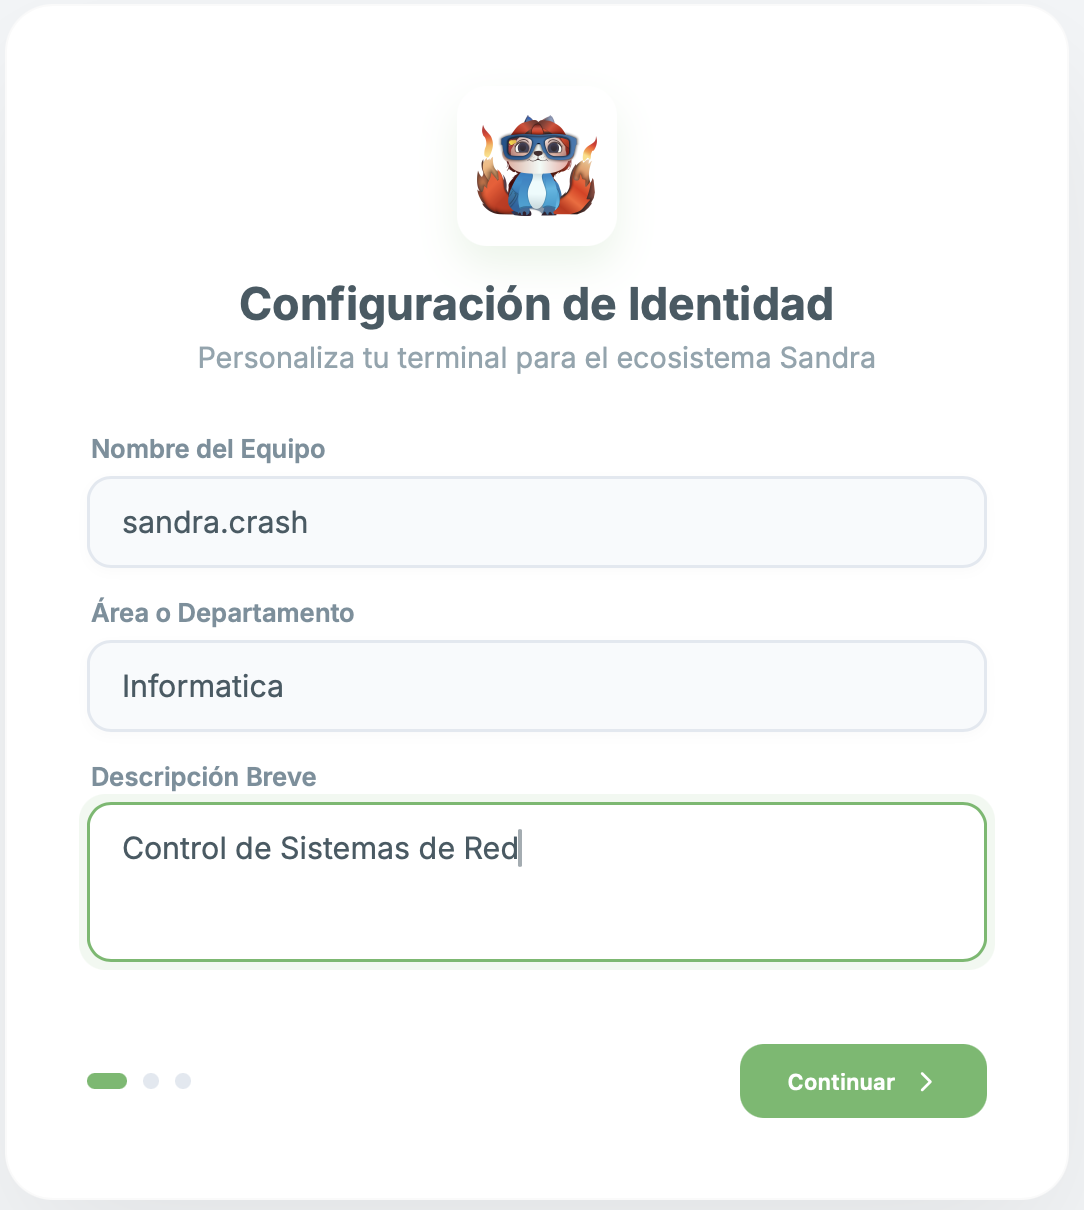
\includegraphics[width=0.5\textwidth]{anexos/2 config.png}
\caption{Pantalla de configuracion inicial de identidad}
\label{fig:config-inicial}
\end{figure}

\subsection{Campos de Configuracion}

La pantalla de configuracion inicial solicita la siguiente informacion:

\begin{table}[H]
\centering
\begin{tabular}{p{4cm}p{4cm}p{6cm}}
\toprule
\textbf{Campo} & \textbf{Ejemplo} & \textbf{Descripcion} \\
\midrule
Nombre del Equipo & sandra.crash & Identificador unico del nodo \\
Area & Desarrollo & Departamento o unidad organizativa \\
\bottomrule
\end{tabular}
\caption{Campos de configuracion de identidad}
\label{tab:campos-identidad}
\end{table}

\begin{quote}
\textbf{Importancia del Nombre del Equipo}\\
\small
Es vital asignar nombres descriptivos y consistentes con la nomenclatura de tu organizacion. Este nombre aparecera en todos los logs del Monitor de Sistema y sera utilizado para identificar el origen de las operaciones durante auditorias forenses.
\end{quote}

\subsection{Mejores Practicas para la Nomenclatura}

Se recomienda seguir estos patrones para los nombres de equipo:

\begin{itemize}[leftmargin=*]
    \item \textbf{Formato}: \texttt{[ambiente].[usuario]} o \texttt{[ubicacion].[funcion]}
    \item \textbf{Ejemplos validos}:
    \begin{itemize}
        \item \texttt{prod.server01} -- Servidor de produccion
        \item \texttt{dev.carlos} -- Estacion de desarrollo
        \item \texttt{hq.finanzas} -- Equipo de finanzas en sede principal
    \end{itemize}
    \item \textbf{Evitar}: espacios, caracteres especiales o nombres genericos como PC-1 o Equipo
\end{itemize}

\section{Vinculacion del Nodo}
\label{sec:vinculacion}

Una vez configurada la identidad basica, SDC procede a detectar automaticamente el entorno del dispositivo y generar un identificador unico de cliente (Client ID).

\begin{figure}[H]
\centering
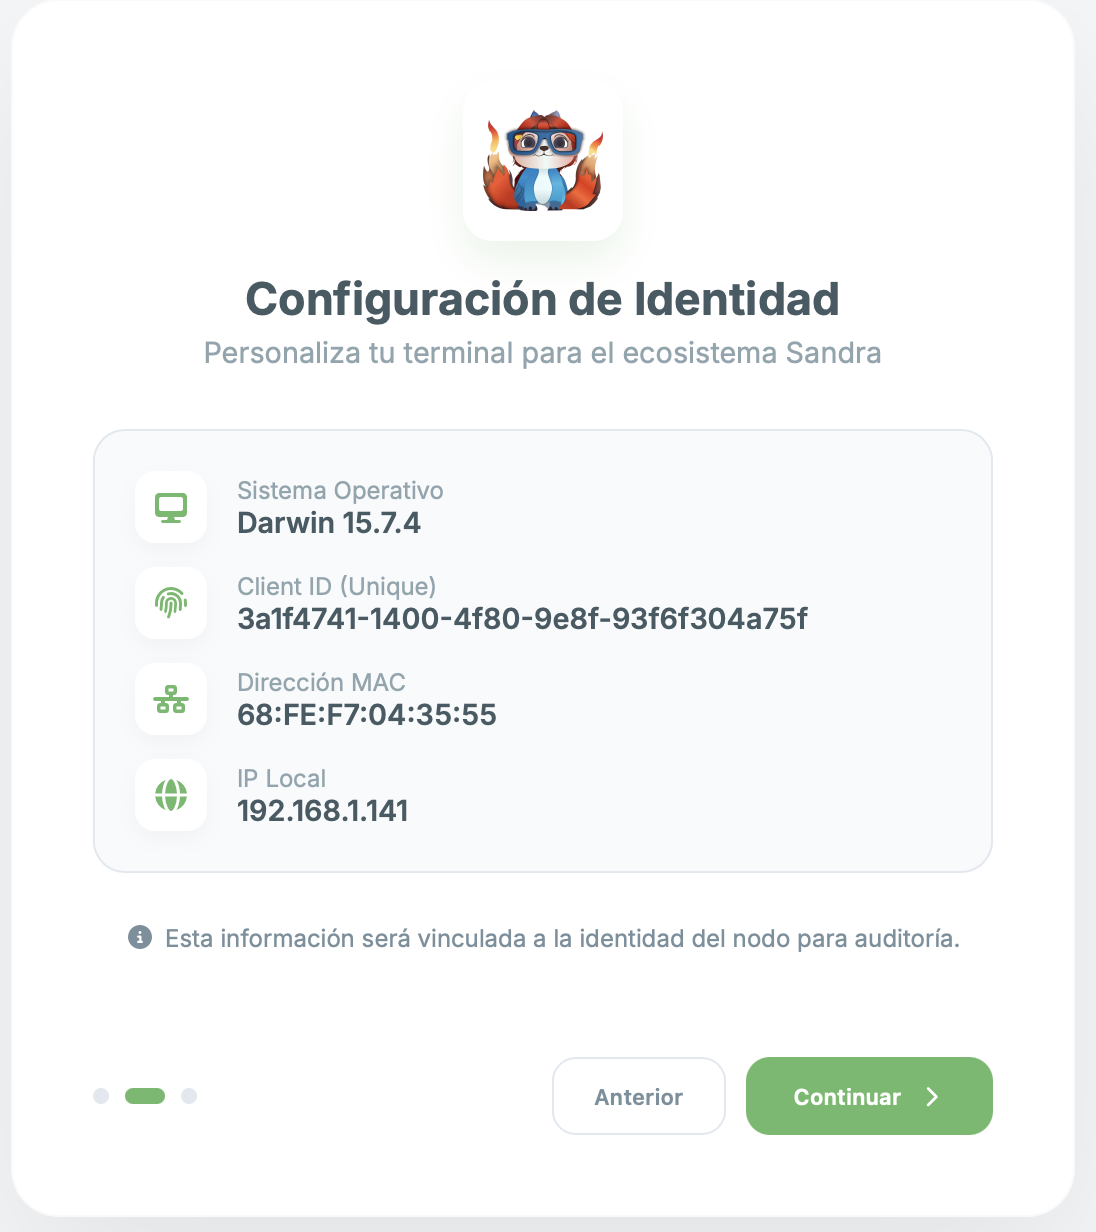
\includegraphics[width=0.5\textwidth]{anexos/3 config.png}
\caption{Pantalla de vinculacion y deteccion de entorno}
\label{fig:vinculacion}
\end{figure}

\subsection{Informacion Detectada Automaticamente}

\begin{table}[H]
\centering
\begin{tabular}{p{4cm}p{3cm}p{7cm}}
\toprule
\textbf{Parametro} & \textbf{Ejemplo} & \textbf{Uso} \\
\midrule
Sistema Operativo & Darwin (macOS) & Compatibilidad y optimizacion \\
IP Local & 192.168.1.100 & Registro de origen de conexiones \\
Direccion MAC & AA:BB:CC:DD:EE:FF & Identificacion fisica del dispositivo \\
Client ID & UUID v4 & Identificador unico criptografico \\
\bottomrule
\end{tabular}
\caption{Informacion de entorno detectada automaticamente}
\label{tab:info-entorno}
\end{table}

\subsection{Generacion del Client ID}

El \keyconcept{Client ID} es un identificador unico generado mediante algoritmos criptograficos que asegura:

\begin{enumerate}[leftmargin=*]
    \item \textbf{Unicidad}: No existen dos dispositivos con el mismo ID en el ecosistema
    \item \textbf{No reversibilidad}: No se puede determinar el hardware original desde el ID
    \item \textbf{Integridad}: Cualquier modificacion del entorno invalida el ID
\end{enumerate}

\begin{quote}
\textbf{Firma Digital de Operaciones}\\
\small
El Client ID se utiliza para firmar digitalmente todas las operaciones realizadas desde el terminal. Esto asegura que cualquier accion (apertura de documento, conexion a servidor, modificacion de configuracion) pueda ser trazada hasta su origen fisico para auditorias futuras.
\end{quote}

\subsection{Proceso de Vinculacion}

El proceso de vinculacion sigue estos pasos:

\begin{enumerate}
    \item \textbf{Deteccion}: SDC escanea automaticamente las interfaces de red y hardware
    \item \textbf{Validacion}: Verifica que el entorno cumple los requisitos minimos de seguridad
    \item \textbf{Generacion}: Crea el Client ID unico vinculado a las caracteristicas del dispositivo
    \item \textbf{Registro}: Almacena de forma segura la huella digital del nodo
    \item \textbf{Confirmacion}: Muestra el resumen de la vinculacion exitosa
\end{enumerate}

\section{Pantalla de Bienvenida}
\label{sec:splash}

Antes de acceder al dashboard principal, SDC presenta una pantalla de bienvenida que confirma la correcta inicializacion del sistema.

\begin{figure}[H]
\centering
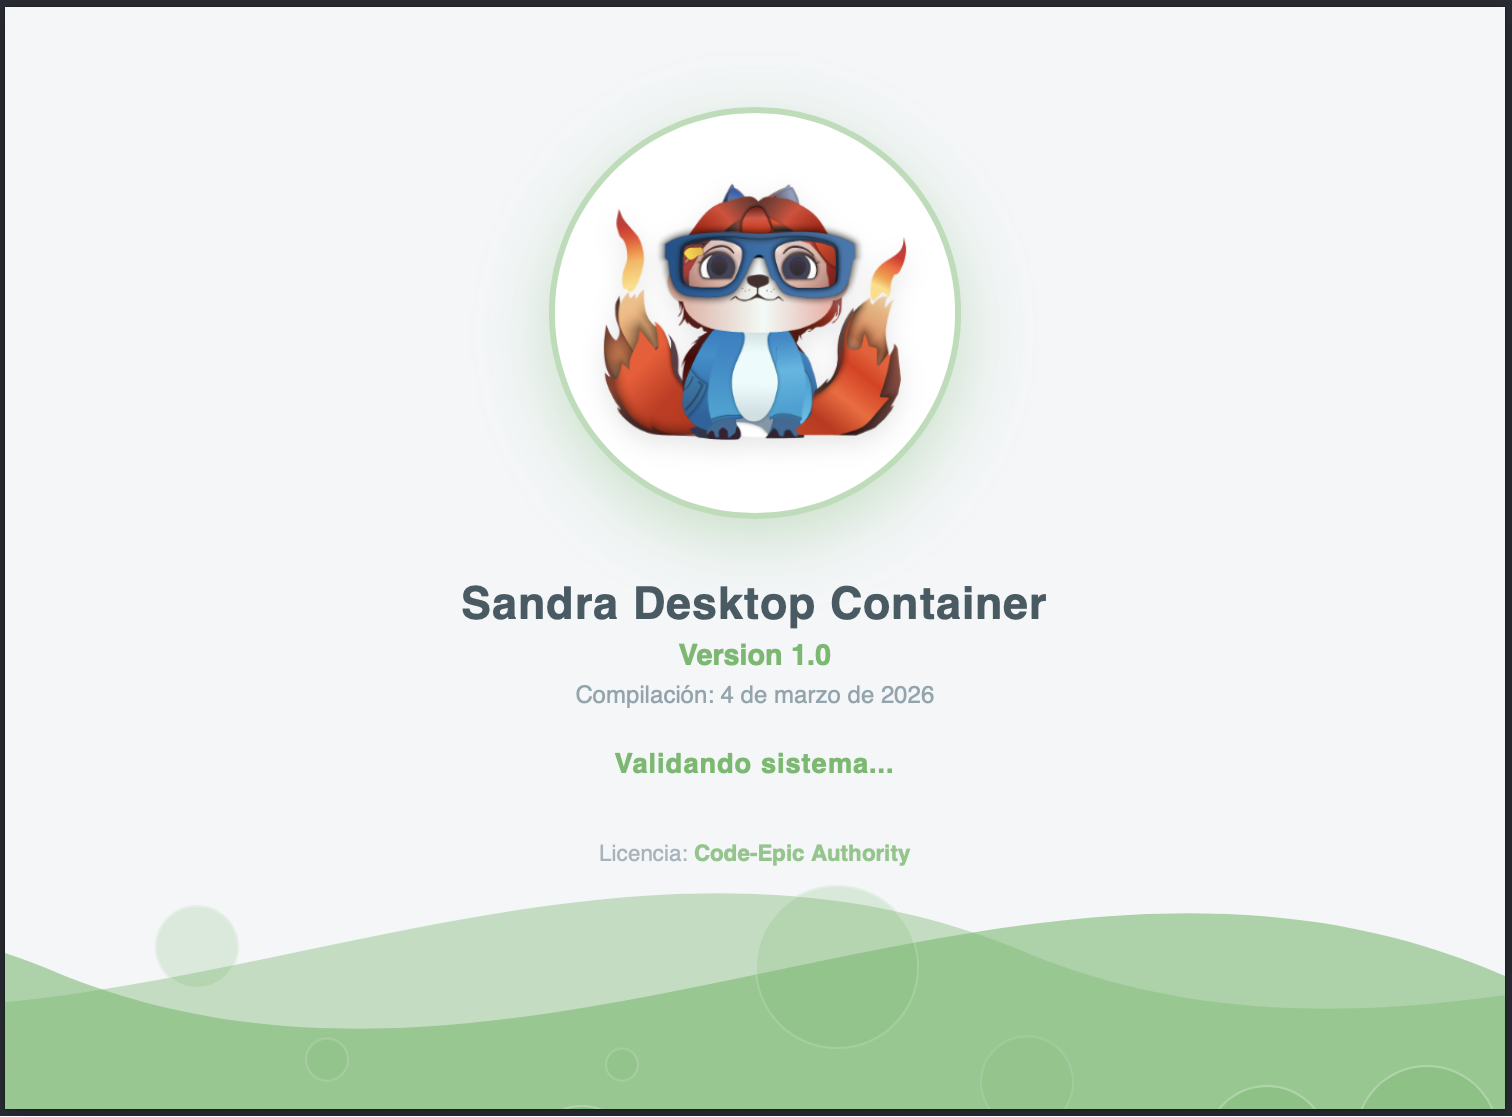
\includegraphics[width=0.9\textwidth]{anexos/1 splash.png}
\caption{Pantalla de bienvenida de SDC}
\label{fig:splash}
\end{figure}

Esta pantalla muestra:
\begin{itemize}[leftmargin=*]
    \item Logo animado de SDC (el mapache con gafas VR)
    \item Version actual del software
    \item Indicador de carga de modulos de seguridad
    \item Verificacion de integridad del sistema
\end{itemize}

\begin{quote}
\textbf{Verificacion de Integridad}\\
\small
Durante la pantalla de bienvenida, SDC realiza una verificacion criptografica de todos los modulos del sistema para detectar posibles alteraciones o corrupciones. Si se detecta alguna anomalia, el sistema se bloqueara y mostrara una alerta de seguridad.
\end{quote}

\section{Resumen del Proceso de Onboarding}

El proceso de onboarding completo sigue estos pasos secuenciales:

\begin{enumerate}
    \item \textbf{Inicio}: Lanzamiento de la aplicacion SDC
    \item \textbf{Configurar Identidad}: Introducir nombre de equipo y area
    \item \textbf{Detectar Entorno}: Escaneo automatico del sistema
    \item \textbf{Generar Client ID}: Creacion del identificador unico
    \item \textbf{Verificar Integridad}: Comprobacion de modulos de seguridad
    \item \textbf{Dashboard}: Acceso al panel principal de control
\end{enumerate}

\section{Solucion de Problemas Comunes}

\begin{table}[H]
\centering
\begin{tabular}{p{5cm}p{8cm}}
\toprule
\textbf{Problema} & \textbf{Solucion} \\
\midrule
Nombre de equipo duplicado & Agregar sufijo numerico o identificador de ubicacion \\
No se detecta IP local & Verificar conexion de red y permisos del sistema \\
Client ID ya existe & Contactar administrador para desvincular dispositivo anterior \\
Error de verificacion & Reiniciar aplicacion; si persiste, reinstalar SDC \\
\bottomrule
\end{tabular}
\caption{Problemas comunes durante el onboarding}
\label{tab:problemas-onboarding}
\end{table}

%======================================================================
% CAPITULO 2: INTERFAZ DE USUARIO Y SANDRA AI
%======================================================================

\chapter{Interfaz de Usuario y Sandra AI}
\label{ch:dashboard}

Este capitulo describe la interfaz principal de \sdc{}, conocida como el Dashboard, y presenta \sandraai{}, el asistente de inteligencia artificial integrado.

\section{El Dashboard Principal}
\label{sec:dashboard}

El panel central de SDC proporciona una vision integral del estado del sistema mediante metricas en tiempo real.

\begin{figure}[H]
\centering
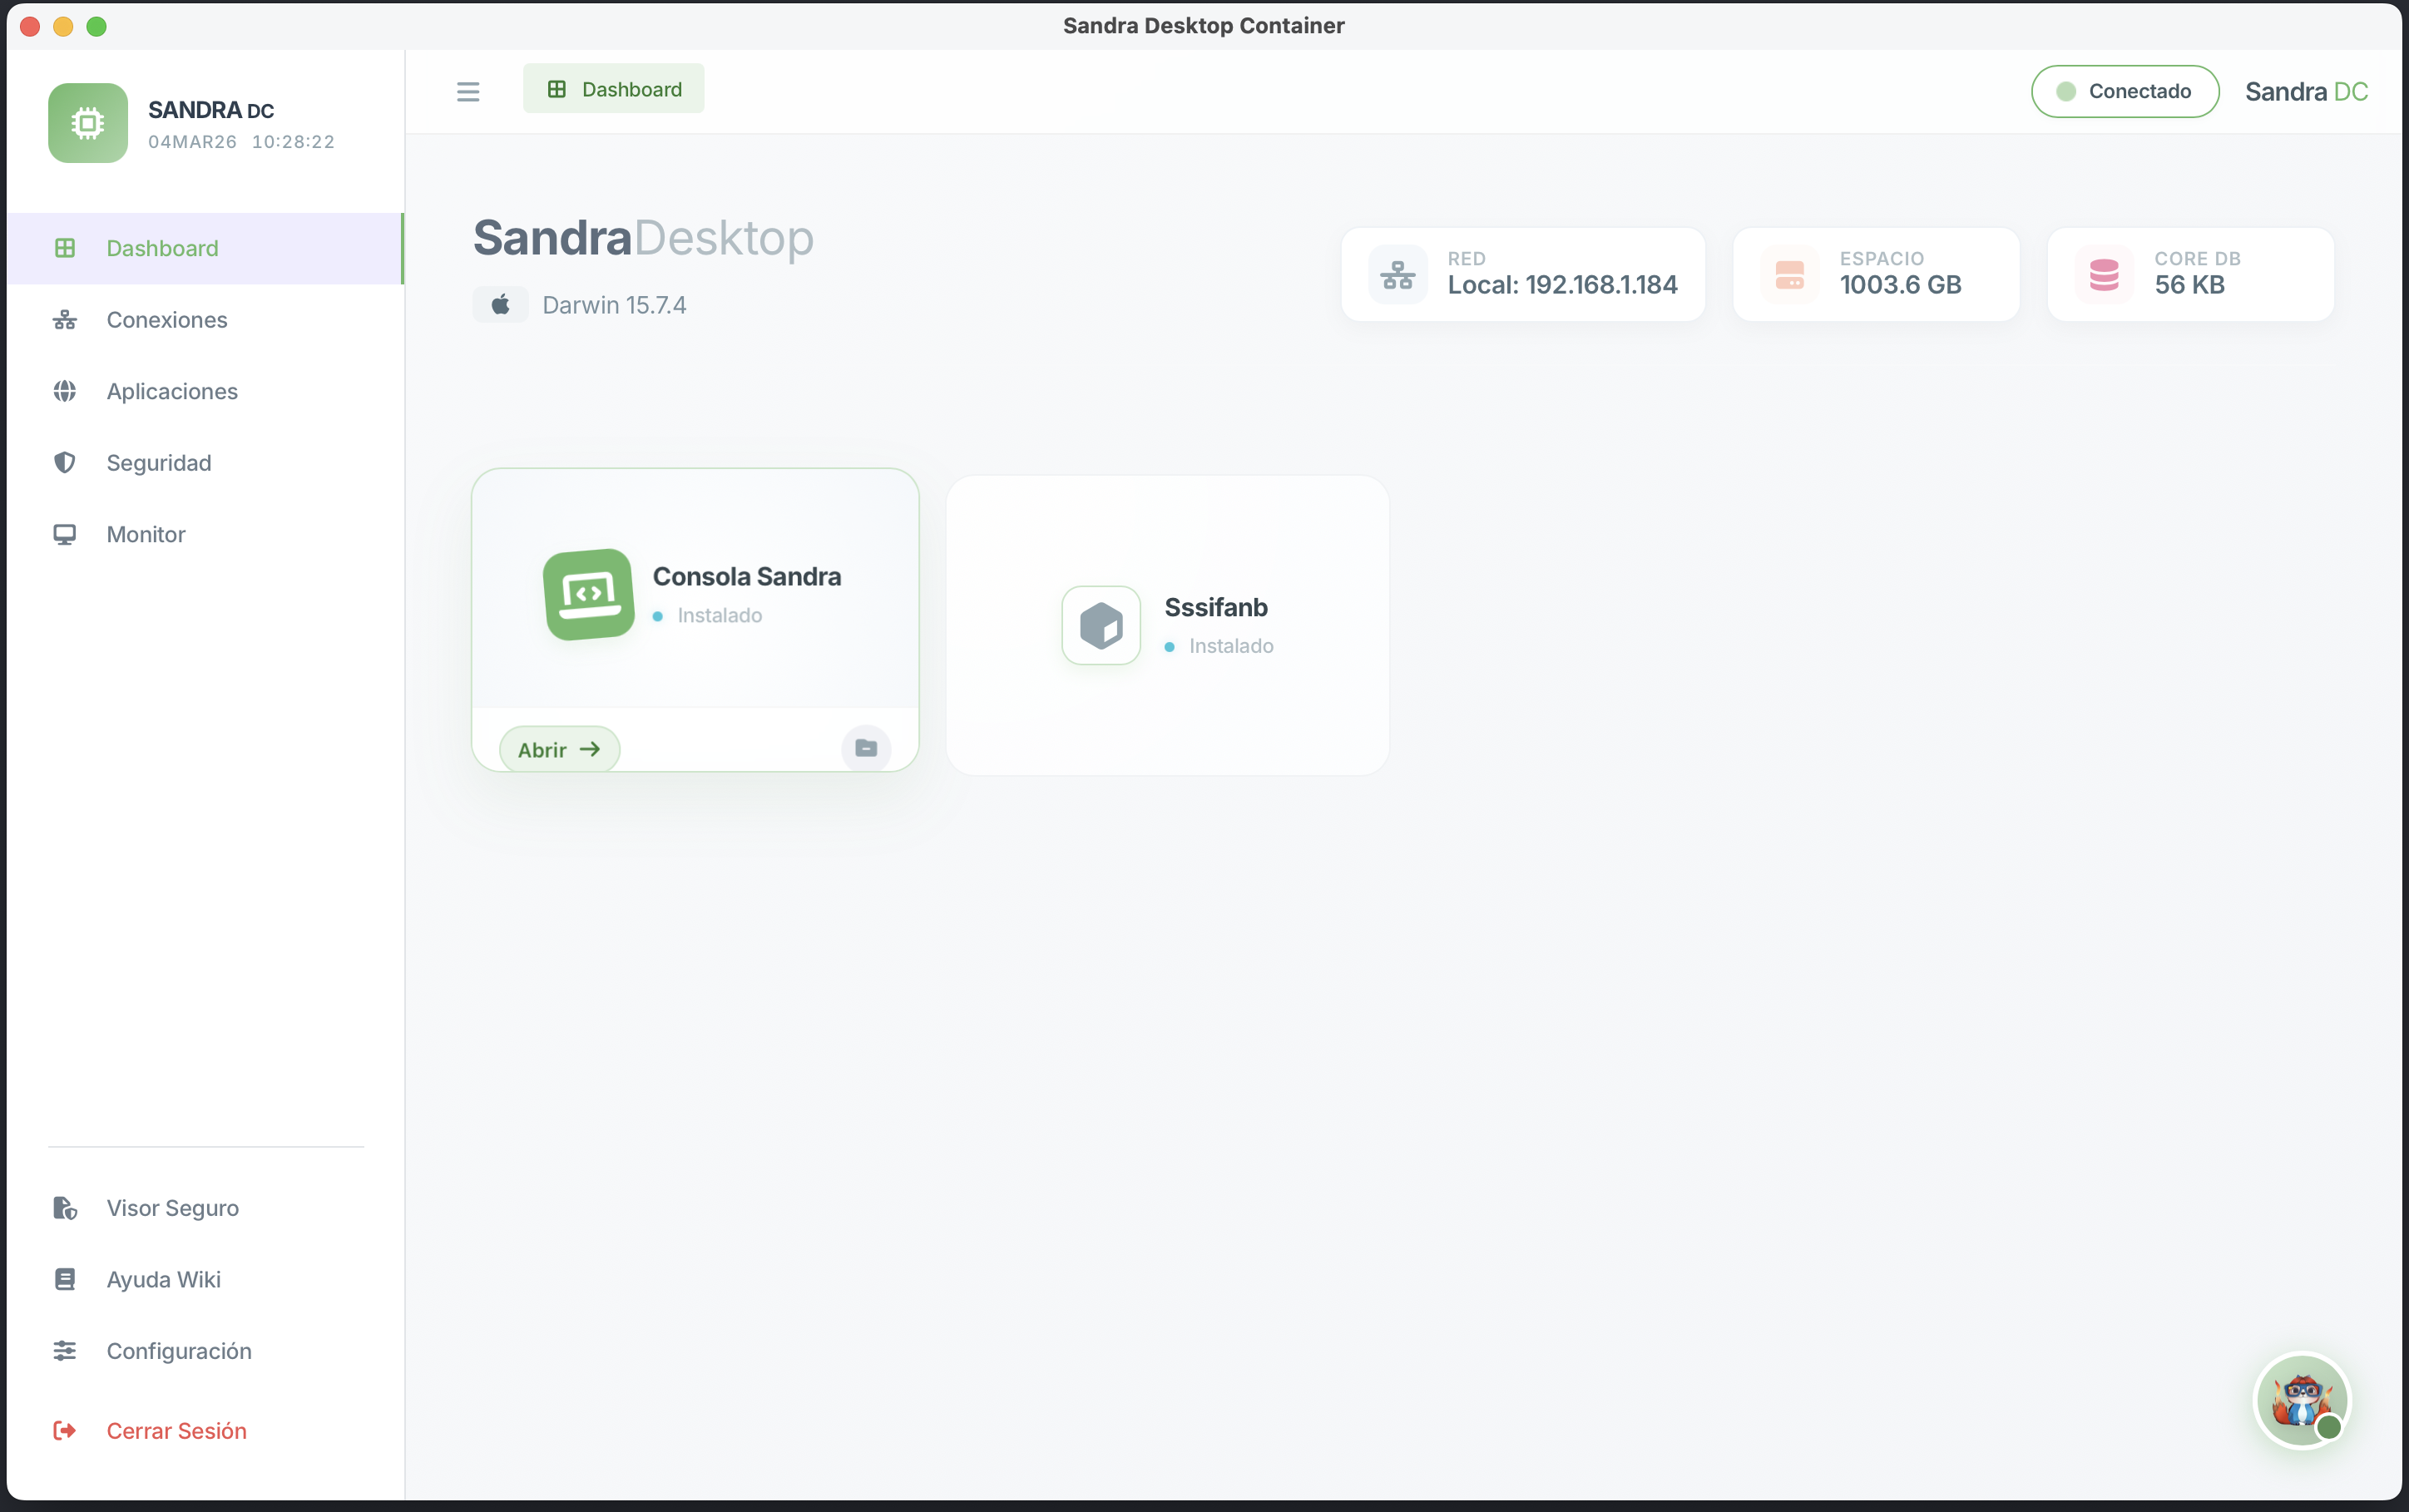
\includegraphics[width=0.95\textwidth]{anexos/4 principal.png}
\caption{Dashboard principal de Sandra Desktop Container}
\label{fig:dashboard}
\end{figure}

\subsection{Panel de Metricas del Sistema}

El dashboard presenta tres metricas fundamentales organizadas en tarjetas visuales:

\begin{table}[H]
\centering
\begin{tabular}{p{4cm}p{3cm}p{8cm}}
\toprule
\textbf{Icono FA} & \textbf{Metrica} & \textbf{Descripcion} \\
\midrule
\texttt{fa-network-wired} & RED & Estado de la conexion local, latencia y throughput \\
\midrule
\texttt{fa-hdd} & ESPACIO & Capacidad disponible en disco para contenedores \\
\midrule
\texttt{fa-database} & CORE DB & Base de datos SQLite interna cifrada \\
\bottomrule
\end{tabular}
\caption{Metricas principales del Dashboard}
\label{tab:metricas-dashboard}
\end{table}

\subsection{Interpretacion de las Metricas}

\subsubsection{Estado de RED}

La metrica de red muestra:
\begin{itemize}[leftmargin=*]
    \item Estado de conexion: Activa/Inactiva
    \item Interfaces detectadas: Ethernet, WiFi
    \item Latencia: Tiempo de respuesta en ms
    \item Throughput: Velocidad de transferencia
\end{itemize}

\begin{quote}
\textbf{Indicadores de Estado:}
\begin{itemize}
    \item \textbf{Verde}: Conexion estable y optima
    \item \textbf{Ambar}: Conexion lenta o inestable
    \item \textbf{Rojo}: Sin conexion o error
\end{itemize}
\end{quote}

\subsubsection{Espacio de Almacenamiento}

El espacio disponible se calcula considerando:
\begin{itemize}[leftmargin=*]
    \item Contenedores activos
    \item Datos temporales
    \item Logs de auditoria
    \item Cache de aplicaciones
\end{itemize}

\begin{quote}
\textbf{Advertencia:} Cuando el espacio desciende por debajo del 20 por ciento, SDC mostrara alerta.
\end{quote}

\section{Asistente Sandra AI}
\label{sec:sandra-ai}

\sandraai{} es una consola de inteligencia artificial ubicada en la esquina inferior derecha del dashboard.

\subsection{Activacion del Asistente}

Para iniciar una conversacion:
\begin{enumerate}[leftmargin=*]
    \item Hacer clic en el icono (clase FA: \texttt{fa-robot}) en la esquina inferior derecha
    \item Escribir la consulta en el campo de texto
    \item Presionar Enter
\end{enumerate}

\subsection{Tipos de Interaccion}

Sandra AI procesa tres categorias de consultas:

\begin{table}[H]
\centering
\begin{tabular}{p{4cm}p{4cm}p{6cm}}
\toprule
\textbf{Categoria} & \textbf{Ejemplo} & \textbf{Respuesta} \\
\midrule
Consultas Tecnicas & Que es una ruta proxy? & Explicacion conceptual \\
\midrule
Comandos Operativos & Crear nueva conexion & Asistente de configuracion \\
\midrule
Diagnostico & Por que no puedo conectarme? & Analisis de logs \\
\bottomrule
\end{tabular}
\caption{Tipos de interaccion con Sandra AI}
\label{tab:tipos-ai}
\end{table}

\subsection{Comandos Predefinidos}

\begin{lstlisting}[language=bash, caption={Comandos de Sandra AI}]
# Gestionar conexiones
- "nueva conexion"
- "listar conexiones"
- "eliminar conexion [nombre]"

# Gestionar aplicaciones
- "nueva aplicacion"
- "abrir aplicacion [nombre]"

# Informacion del sistema
- "estado del sistema"
- "espacio disponible"
- "logs de auditoria"
\end{lstlisting}

\section{Navegacion Principal}
\label{sec:navegacion}

Modulos de la barra lateral:

\begin{table}[H]
\centering
\begin{tabular}{p{3.5cm}p{10cm}}
\toprule
\textbf{Modulo (Icono FA)} & \textbf{Descripcion} \\
\midrule
\texttt{fa-th-large} Dashboard & Panel principal con metricas \\
\texttt{fa-code} Aplicaciones & Micro-aplicaciones desplegadas \\
\texttt{fa-plug} Conexiones & Servidores remotos \\
\texttt{fa-shield-alt} Seguridad & Politicas y auditoria \\
\texttt{fa-eye} Visor & Documentos seguros \\
\texttt{fa-cog} Configuracion & Preferencias \\
\bottomrule
\end{tabular}
\caption{Modulos de navegacion de SDC}
\label{tab:modulos-navegacion}
\end{table}

\subsection{Accesos Directos}

\begin{itemize}[leftmargin=*]
    \item \texttt{fa-plus} Nueva Conexion
    \item \texttt{fa-plus} Nueva Aplicacion
    \item \texttt{fa-sync} Sincronizar
    \item \texttt{fa-history} Auditoria
\end{itemize}

\section{Personalizacion del Dashboard}

\subsection{Temas de Color}

\begin{itemize}[leftmargin=*]
    \item \textbf{Tema Claro}: Paleta Sandra Teal Soft (default)
    \item \textbf{Tema Oscuro}: Optimizado para uso nocturno
    \item \textbf{Tema Alto Contraste}: Accesibilidad
\end{itemize}


\part{Gestión y Operaciones}
%======================================================================
% CAPITULO 3: GESTION DE CONEXIONES Y APLICACIONES
%======================================================================

\chapter{Gestion de Conexiones y Aplicaciones}
\label{ch:gestion}

\sdc{} permite gestionar multiples servidores y convertir servicios web en aplicaciones de escritorio independientes. Este capitulo detalla el proceso de configuracion de conexiones y despliegue de aplicaciones.

\section{Perfiles de Conexion}
\label{sec:conexiones}

El sistema permite gestionar multiples servidores remotos mediante perfiles de conexion configurables.

\begin{figure}[H]
\centering
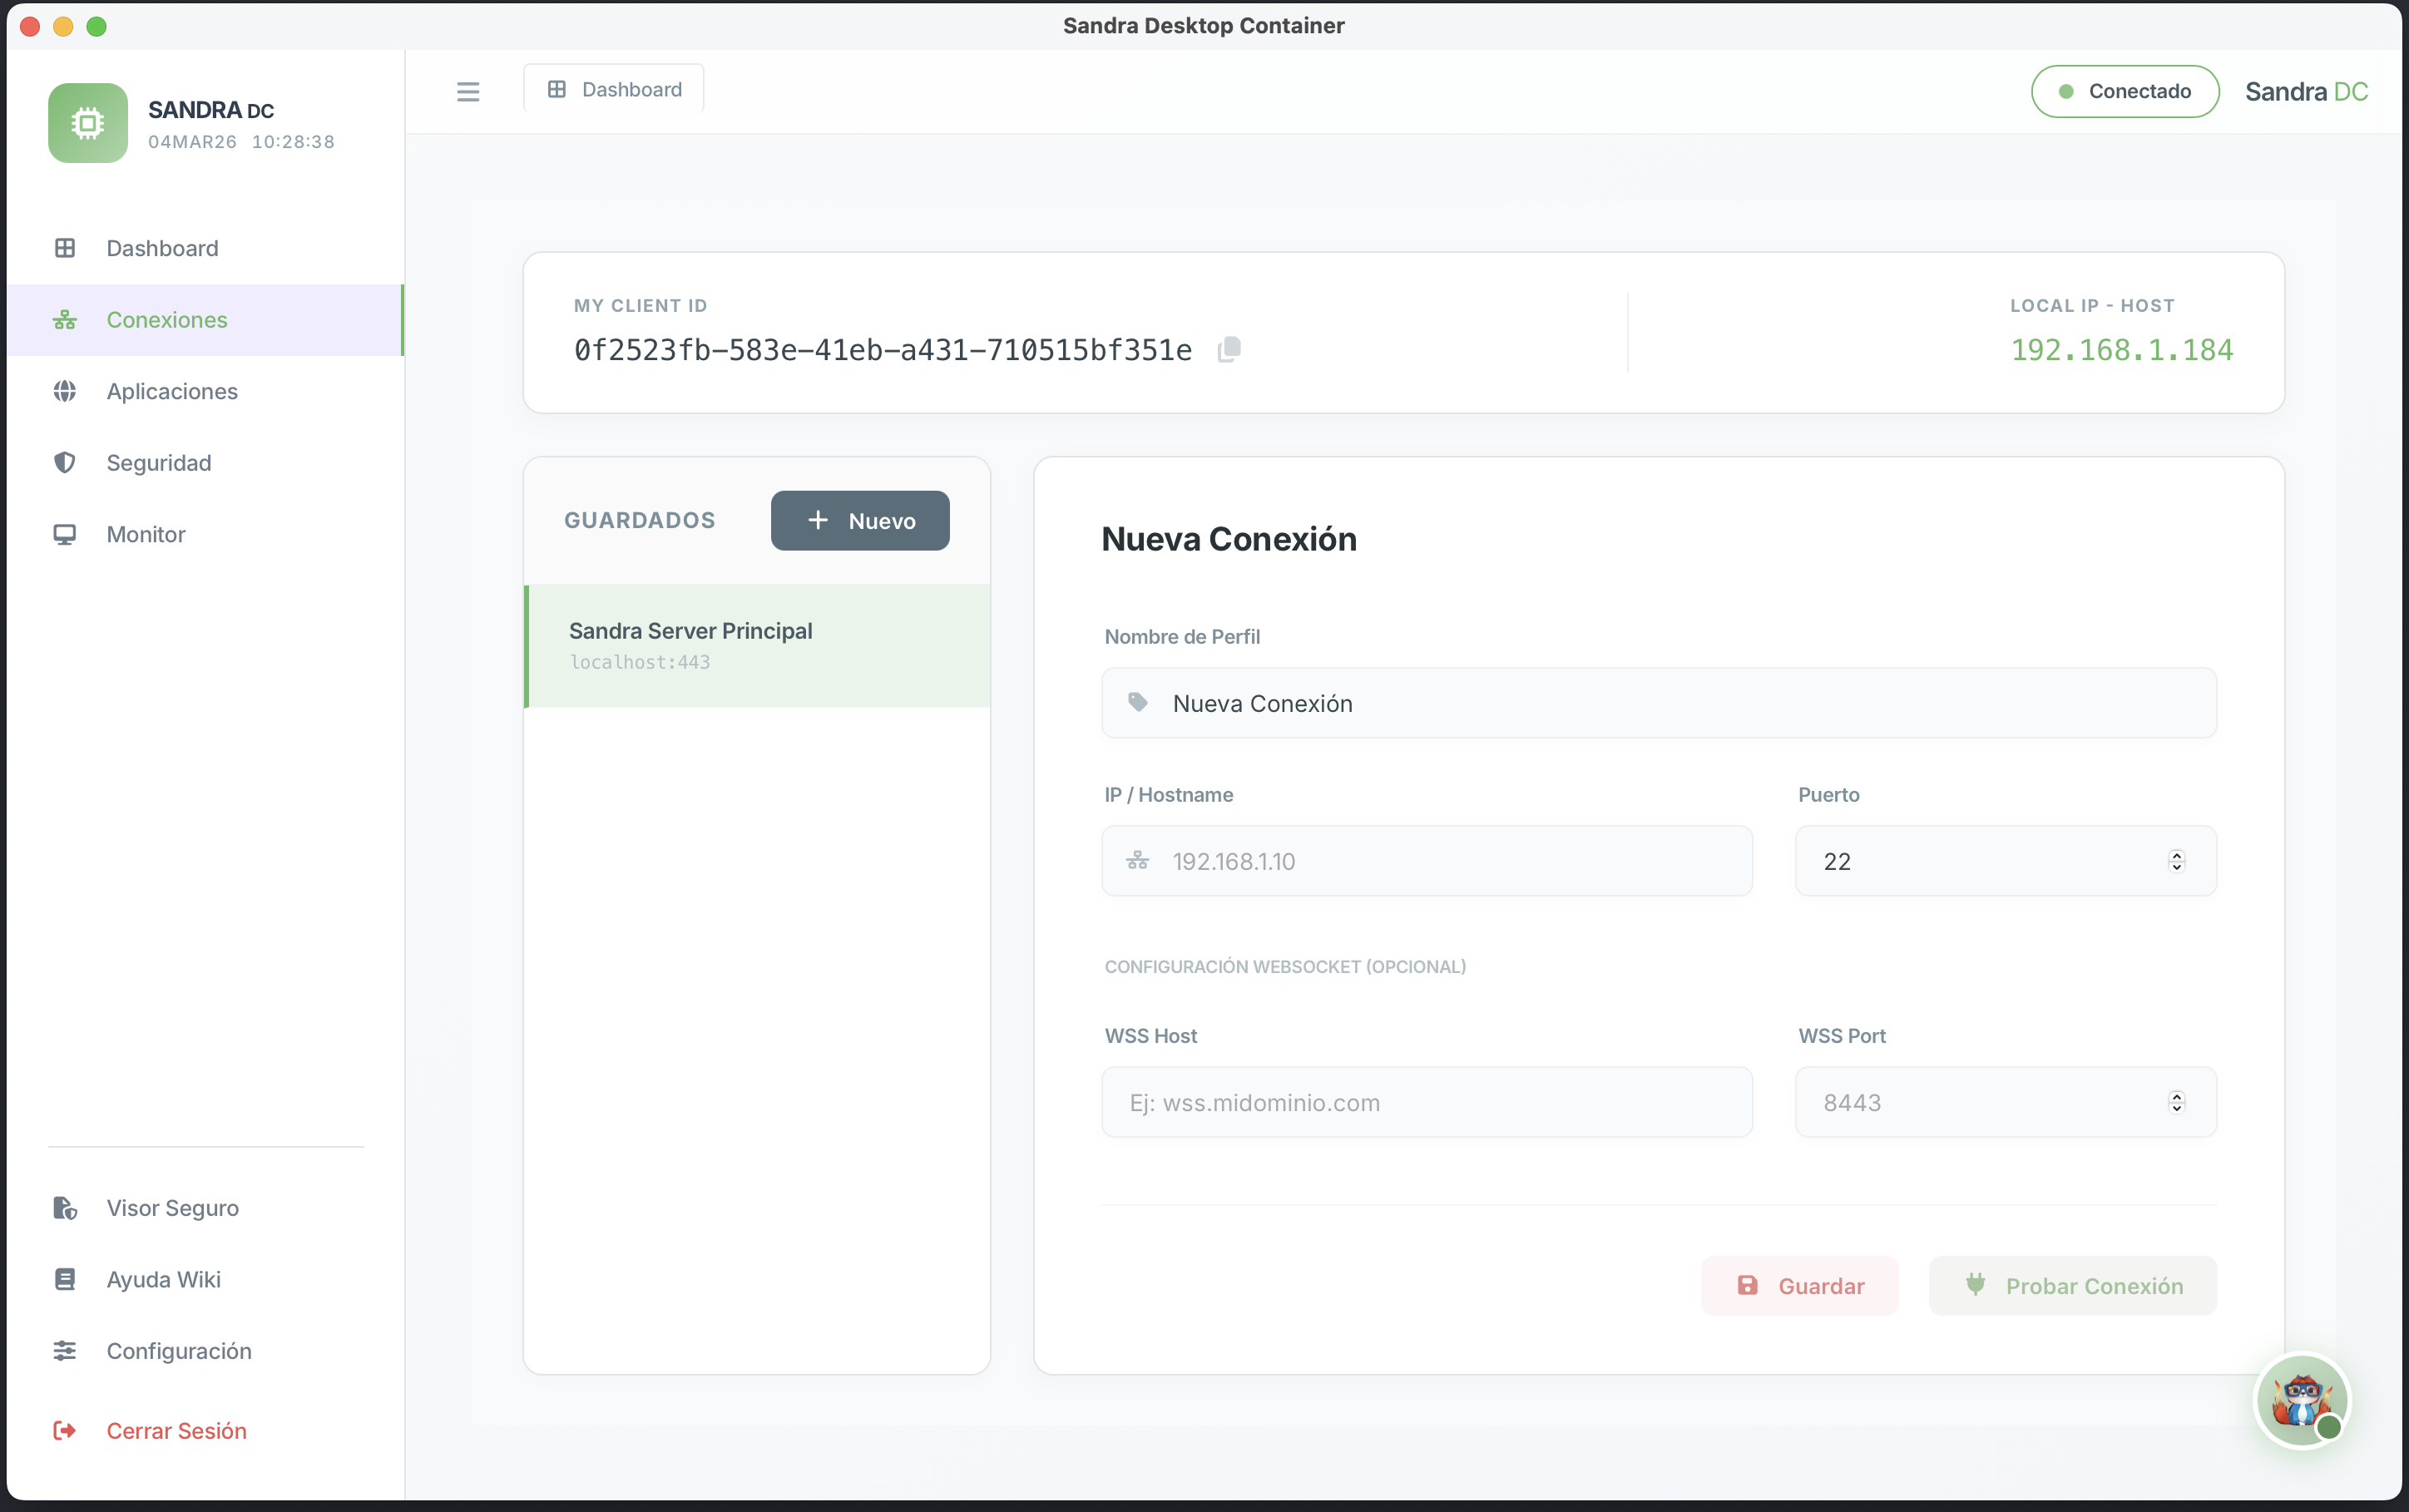
\includegraphics[width=0.95\textwidth]{anexos/5 conexion.png}
\caption{Interfaz de gestion de conexiones}
\label{fig:conexiones}
\end{figure}

\subsection{Creacion de Nueva Conexion}

Para establecer una nueva conexion a un servidor:

\begin{enumerate}[leftmargin=*]
    \item En el dashboard, hacer clic en Nueva Conexion
    \item Completar el formulario de configuracion basica
    \item Configurar opciones de seguridad (recomendado: WSS)
    \item Probar la conexion antes de guardar
    \item Asignar un nombre descriptivo al perfil
\end{enumerate}

\subsection{Parametros de Conexion}

\begin{table}[H]
\centering
\begin{tabular}{p{4cm}p{3cm}p{6cm}}
\toprule
\textbf{Parametro} & \textbf{Ejemplo} & \textbf{Descripcion} \\
\midrule
Host & servidor.com & Direccion IP o dominio \\
Puerto & 8443 & Puerto de escucha \\
Protocolo & WSS / WS & WebSocket Secure o WebSocket plano \\
Nombre & Produccion & Identificador del perfil \\
\bottomrule
\end{tabular}
\caption{Parametros de configuracion de conexion}
\label{tab:parametros-conexion}
\end{table}

\begin{quote}
\textbf{Seguridad de Conexiones}\\
Se recomienda utilizar siempre WSS (WebSocket Secure) en el puerto 8443 o superior. Las conexiones WS (sin cifrar) solo deben usarse en entornos de desarrollo controlados.
\end{quote}

\section{Despliegue de Aplicaciones}
\label{sec:aplicaciones}

Una de las caracteristicas distintivas de SDC es la capacidad de convertir servicios web en aplicaciones de escritorio independientes.

\begin{figure}[H]
\centering
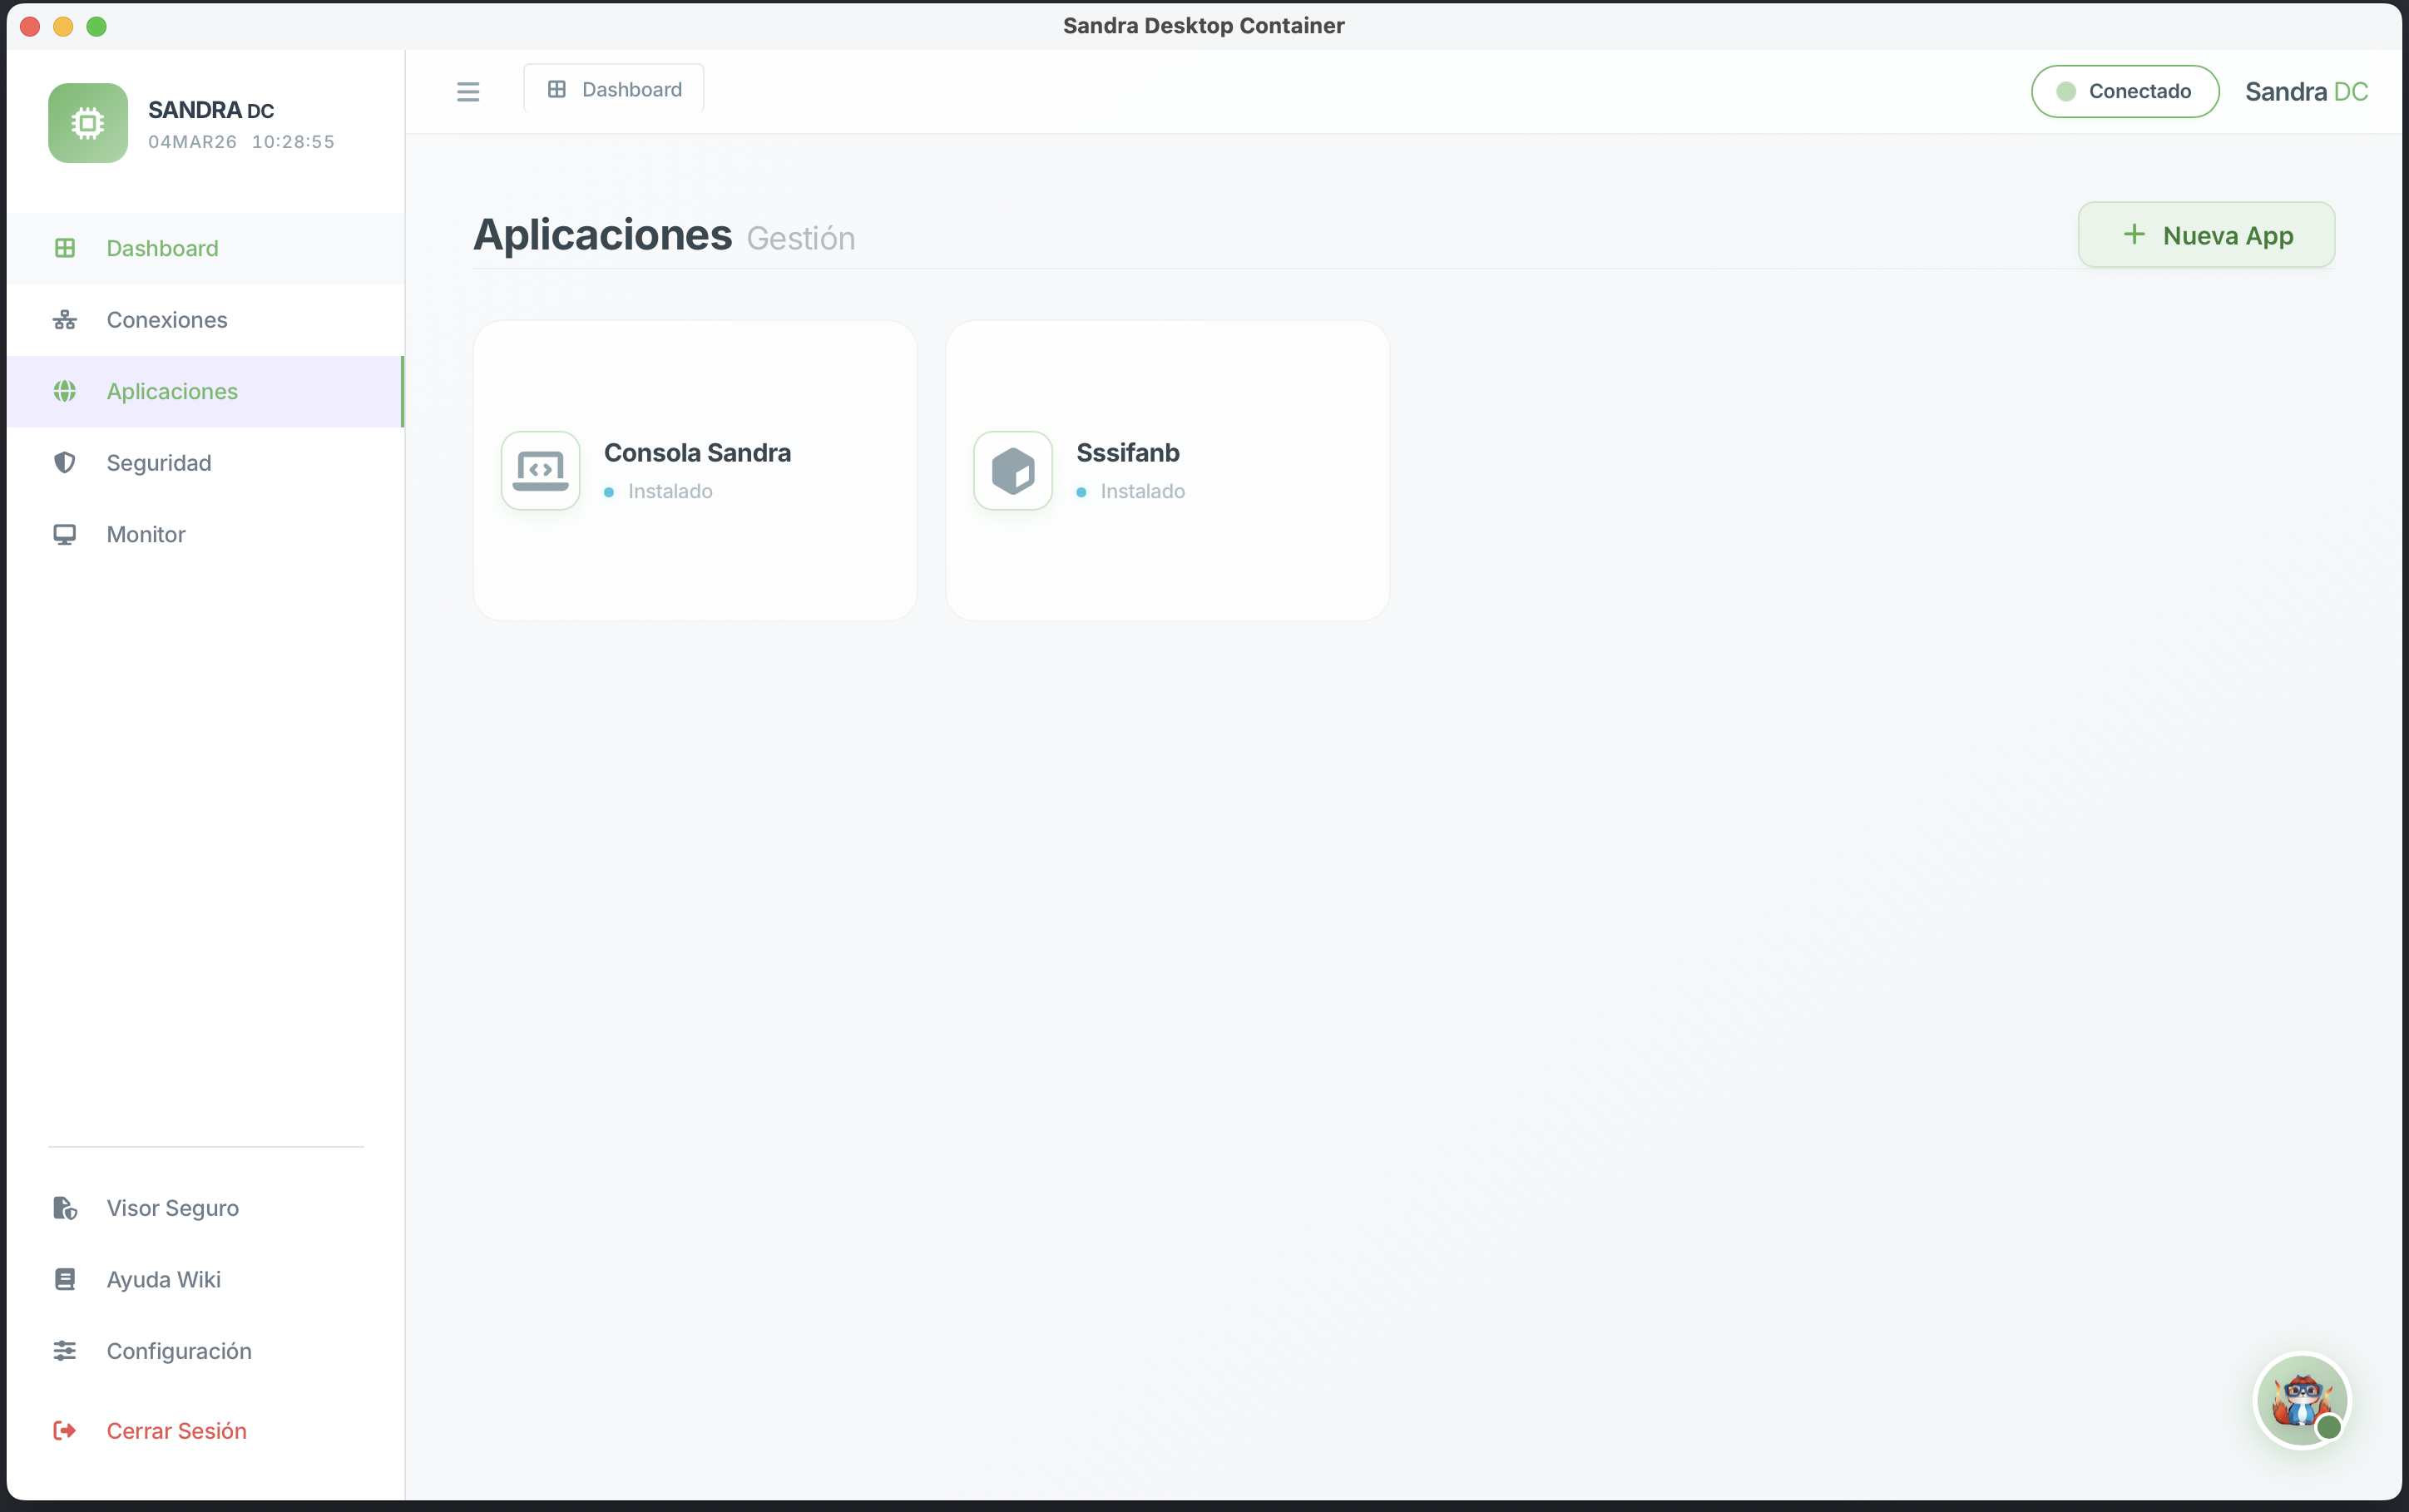
\includegraphics[width=0.95\textwidth]{anexos/6 aplicaciones.png}
\caption{Formulario de creacion de nueva aplicacion}
\label{fig:aplicaciones}
\end{figure}

\subsection{Modos de Despliegue}

\begin{table}[H]
\centering
\begin{tabular}{p{4cm}p{9cm}}
\toprule
\textbf{Modo} & \textbf{Descripcion} \\
\midrule
Proxy Seguro & Enmascara la IP real del contenedor mediante tuneles cifrados. Ideal para aplicaciones criticas. \\
\midrule
Navegacion Libre & Acceso directo sin tuneles de seguridad adicionales. Para aplicaciones internas de baja criticidad. \\
\bottomrule
\end{tabular}
\caption{Modos de despliegue de aplicaciones}
\label{tab:modos-despliegue}
\end{table}

\subsection{Repositorio Fuente}

SDC permite vincular aplicaciones a repositorios de codigo para habilitar despliegues automaticos:

\begin{lstlisting}[language=bash, caption={Configuracion de Repositorio}]
# Soporte para:
- GitHub (github.com/usuario/repo)
- GitLab (gitlab.com/usuario/repo)
- Bitbucket (bitbucket.org/usuario/repo)
- Repositorio privado (URL + credenciales)

# Opciones de despliegue automatico:
- Actualizar al iniciar
- Actualizar manualmente
- Actualizar programada (cron)
\end{lstlisting}

\begin{quote}
\textbf{Despliegue Automatico}\\
Cuando se activa el despliegue automatico, SDC verifica cambios en el repositorio cada 5 minutos y notifica al usuario cuando hay nueva version disponible.
\end{quote}

\section{Lista de Conexiones Activas}
\label{sec:conexiones-activas}

El panel de conexiones activas permite monitorear todas las conexiones establecidas.

\begin{figure}[H]
\centering
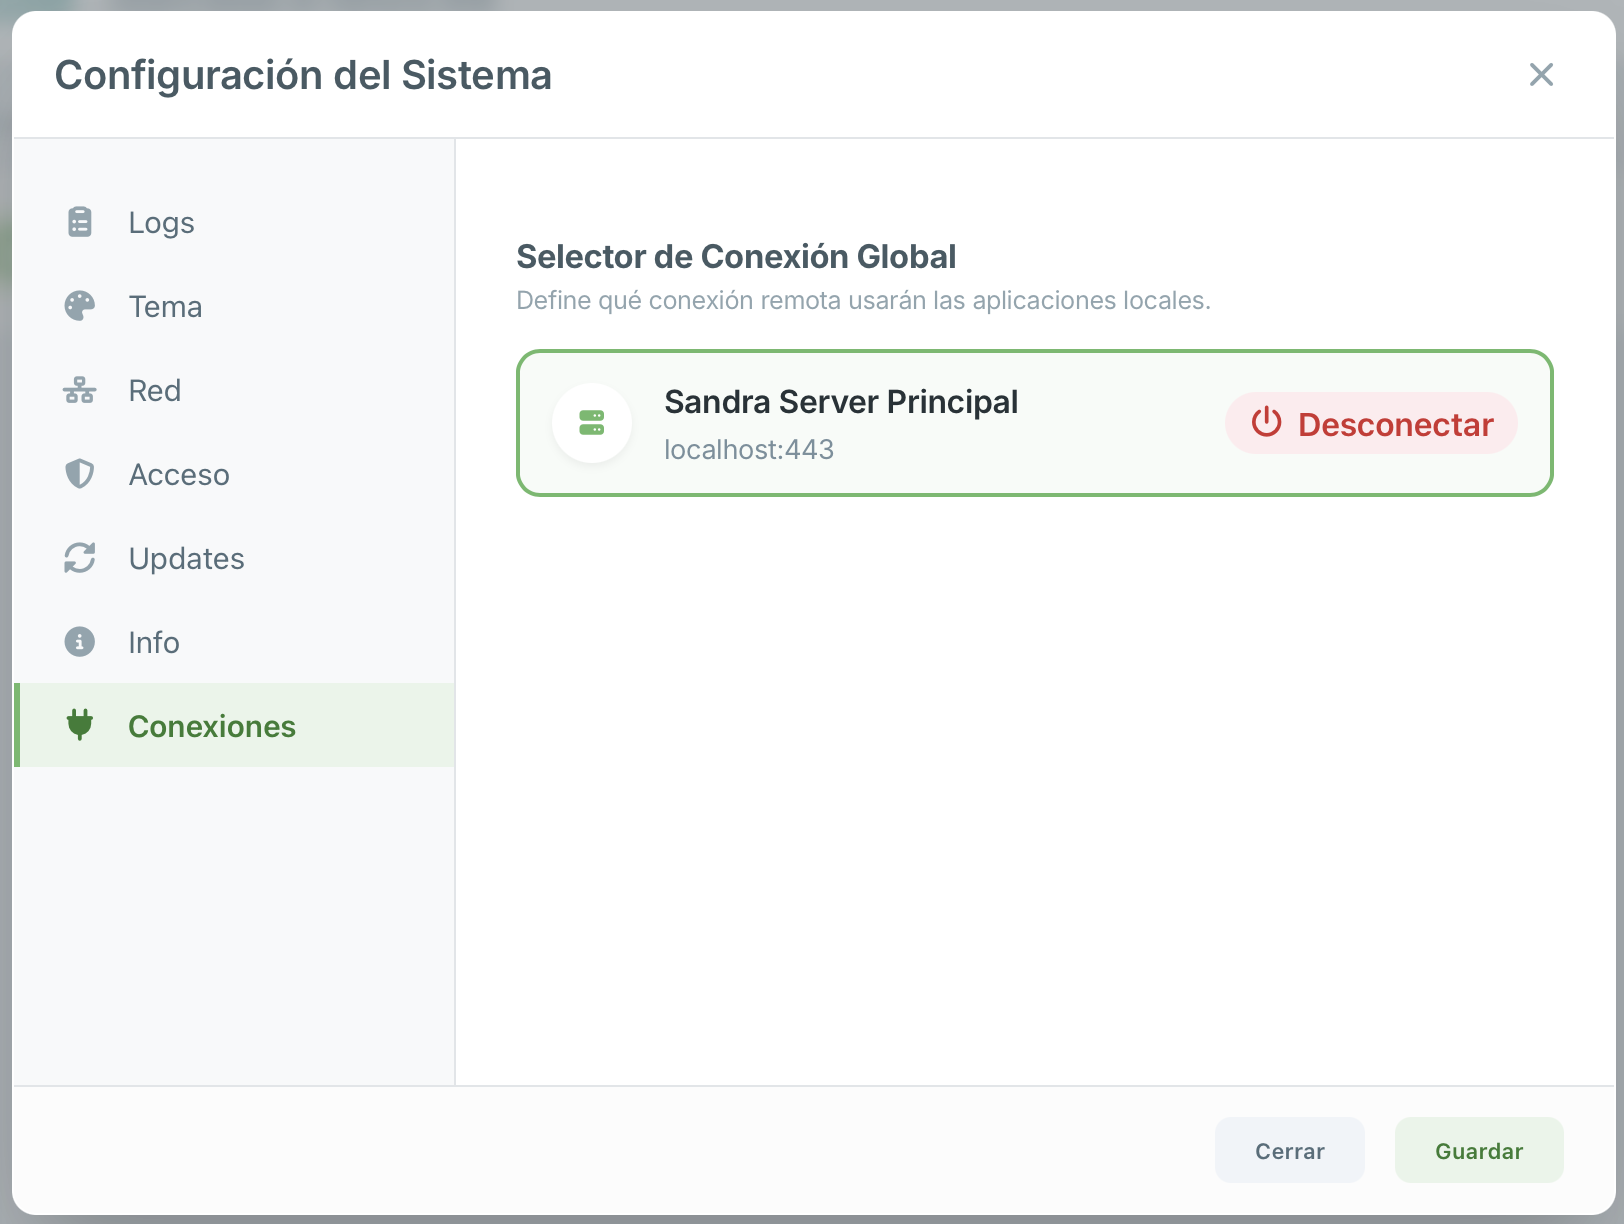
\includegraphics[width=0.95\textwidth]{anexos/16 conexiones activas.png}
\caption{Monitor de conexiones activas}
\label{fig:conexiones-activas}
\end{figure}

\subsection{Informacion Visualizada}

Para cada conexion activa, el sistema muestra:

\begin{itemize}[leftmargin=*]
    \item Estado (Verde: Activa, Rojo: Error, Gris: Inactiva)
    \item Nombre del perfil de conexion
    \item Host y puerto destino
    \item Tiempo de actividad (uptime)
    \item Latencia actual en ms
    \item Bytes transferidos
\end{itemize}

\section{Gestión del Monitor del Sistema}
\label{sec:monitor}

El modulo de monitoreo proporciona metricas detalladas de bajo nivel.

\begin{figure}[H]
\centering
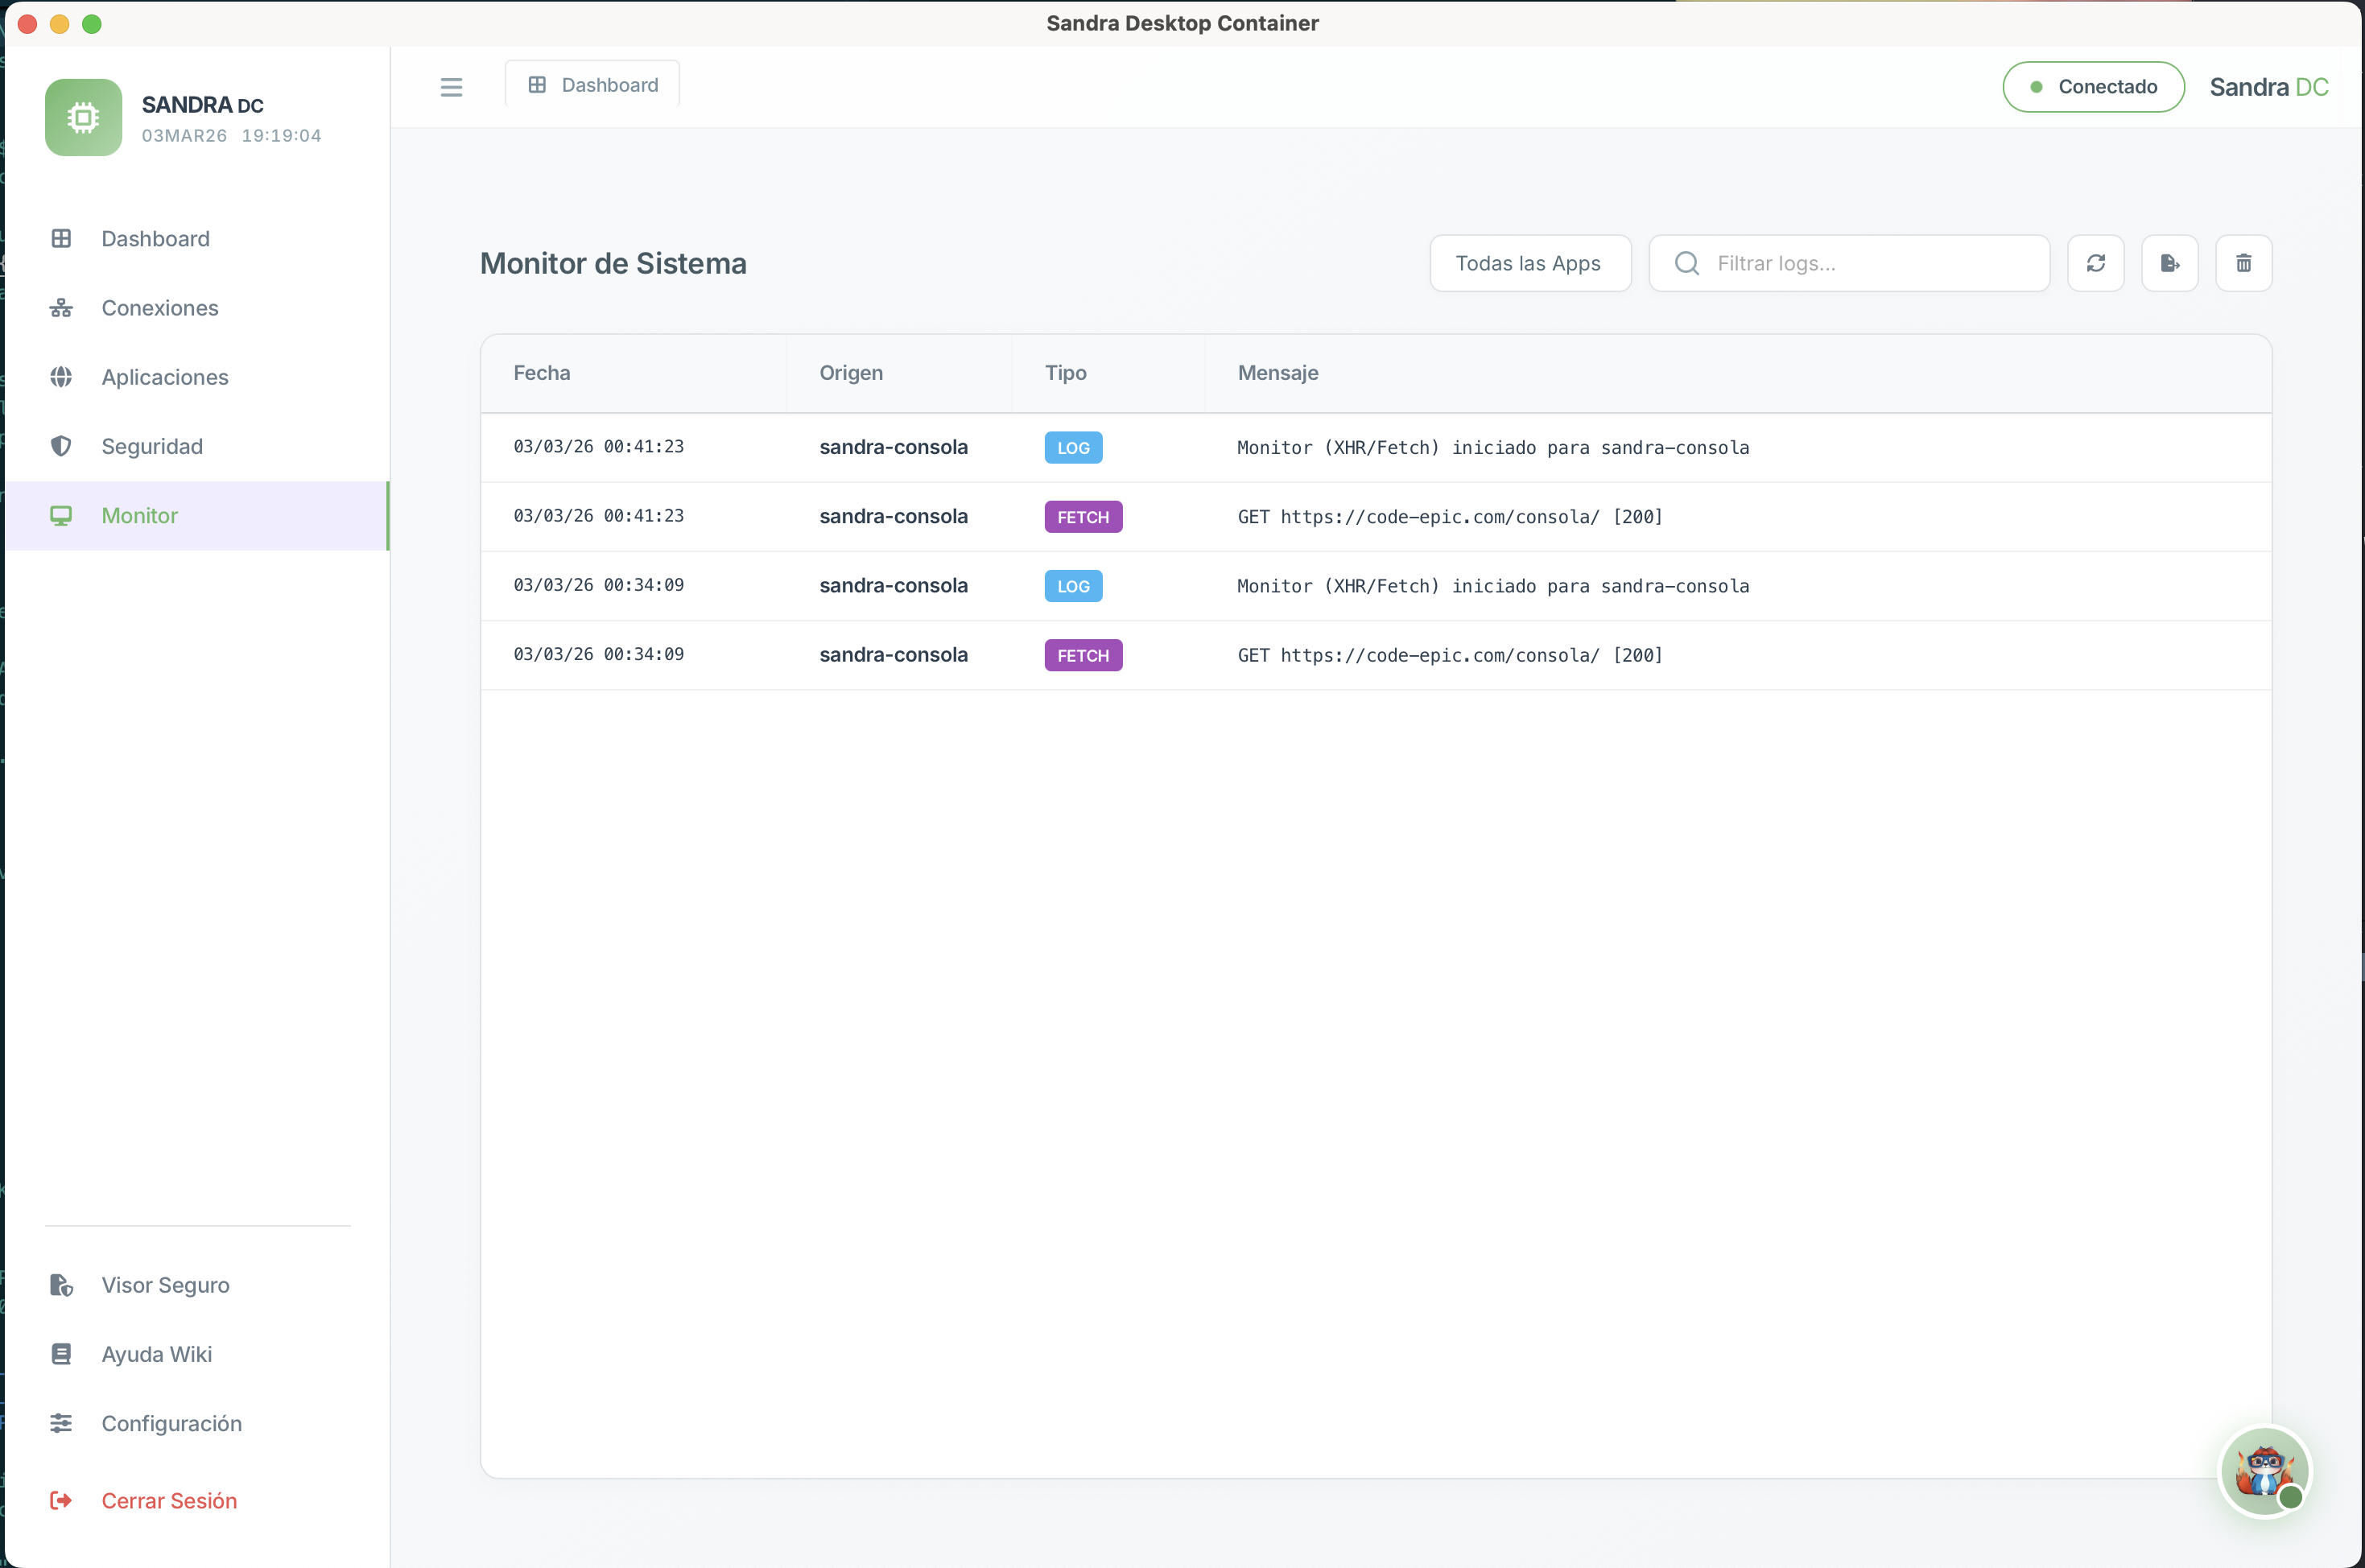
\includegraphics[width=0.95\textwidth]{anexos/10 monitor.png}
\caption{Monitor del sistema en tiempo real}
\label{fig:monitor}
\end{figure}

\subsection{Metricas de Hardware}

\begin{table}[H]
\centering
\begin{tabular}{p{3cm}p{5cm}p{5cm}}
\toprule
\textbf{Recurso} & \textbf{Metrica} & \textbf{Umbral de Alerta} \\
\midrule
CPU & Uso porcentual por nucleo & Mayor a 90 por ciento sostenido \\
RAM & Uso en GB / Total disponible & Mayor a 85 por ciento uso \\
Red & Paquetes/s y bytes/s & Latencia mayor a 500ms \\
Disco & I/O operaciones por segundo & Tiempo mayor a 100ms \\
\bottomrule
\end{tabular}
\caption{Metricas monitoreadas del sistema}
\label{tab:metricas-monitor}
\end{table}

\subsection{Inspector de Red}

Herramienta de transparencia que permite auditar el trafico de red:

\begin{itemize}[leftmargin=*]
    \item Interceptacion pasiva de peticiones Fetch/XHR
    \item Visualizacion de headers y payloads
    \item Filtrado por dominio, metodo HTTP o tipo de contenido
    \item Exportacion de logs para analisis forense
\end{itemize}

\begin{quote}
\textbf{Interceptacion Licita}\\
El Inspector de Red actua como herramienta de transparencia para auditores de seguridad. Su funcionamiento esta limitado al trafico generado por aplicaciones SDC.
\end{quote}

%======================================================================
% CAPITULO 4: SEGURIDAD Y POLITICAS
%======================================================================

\chapter{Seguridad y Politicas de Proteccion}
\label{ch:seguridad}

La seguridad es el pilar fundamental de \sdc{}. Este capitulo detalla la configuracion de politicas de seguridad, gestion de contrasenas, niveles de auditoria y configuracion de rutas proxy seguras.

\section{Configuracion de Seguridad}
\label{sec:config-seguridad}

El panel de seguridad centraliza todas las configuraciones relacionadas con la proteccion del sistema y los datos.

\begin{figure}[H]
\centering
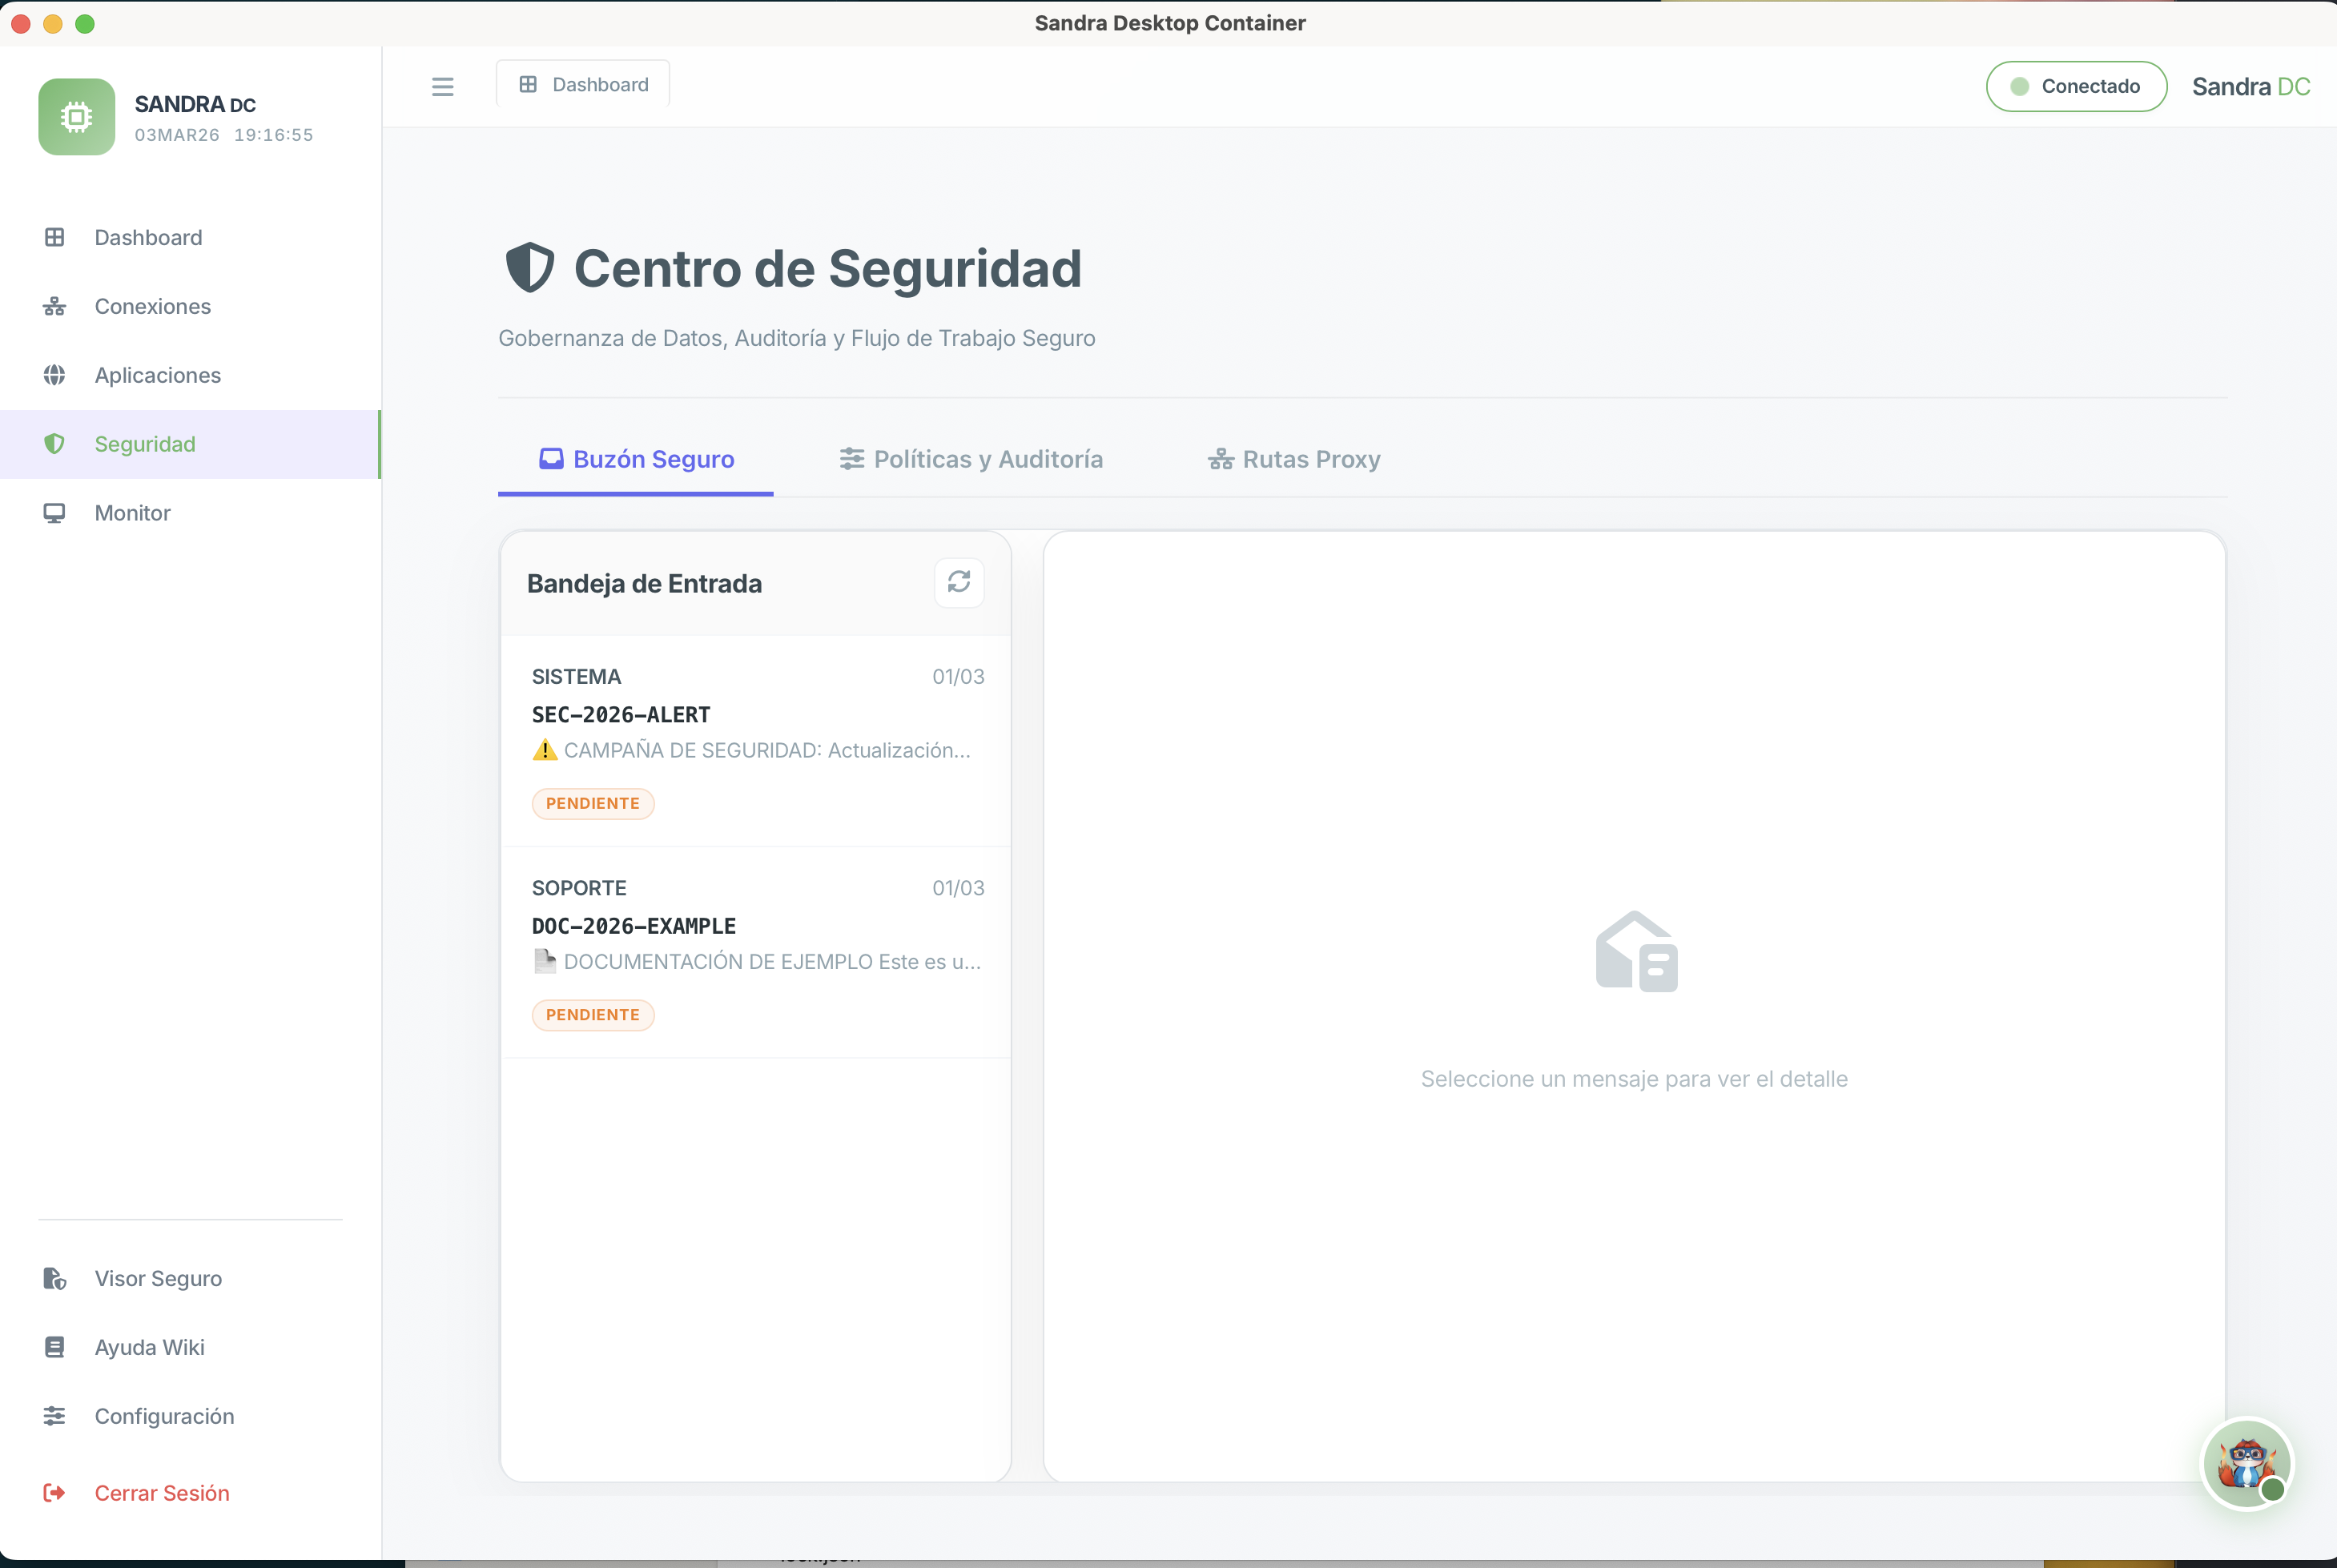
\includegraphics[width=0.95\textwidth]{anexos/7 seguridad.png}
\caption{Panel principal de configuracion de seguridad}
\label{fig:seguridad}
\end{figure}

\subsection{Niveles de Seguridad Predefinidos}

SDC ofrece tres perfiles de seguridad:

\begin{table}[H]
\centering
\begin{tabular}{p{3cm}p{5cm}p{5cm}}
\toprule
\textbf{Nivel} & \textbf{Caracteristicas} & \textbf{Recomendado Para} \\
\midrule
Basico & Auditoria minima, politicas estandar, logs locales & Entornos de desarrollo \\
\midrule
Estandar & Auditoria completa, contrasenas robustas, encriptacion AES-256 & Operaciones empresariales \\
\midrule
Critico & Auditoria en tiempo real, contrasenas de alta entropia, MFA, logs inmutables & Datos clasificados \\
\bottomrule
\end{tabular}
\caption{Niveles de seguridad predefinidos}
\label{tab:niveles-seguridad}
\end{table}

\section{Politicas de Contrasenas}
\label{sec:politicas-password}

Las politicas de contrasenas permiten definir expresiones regulares (regex) que validan la complejidad de las credenciales.

\begin{figure}[H]
\centering
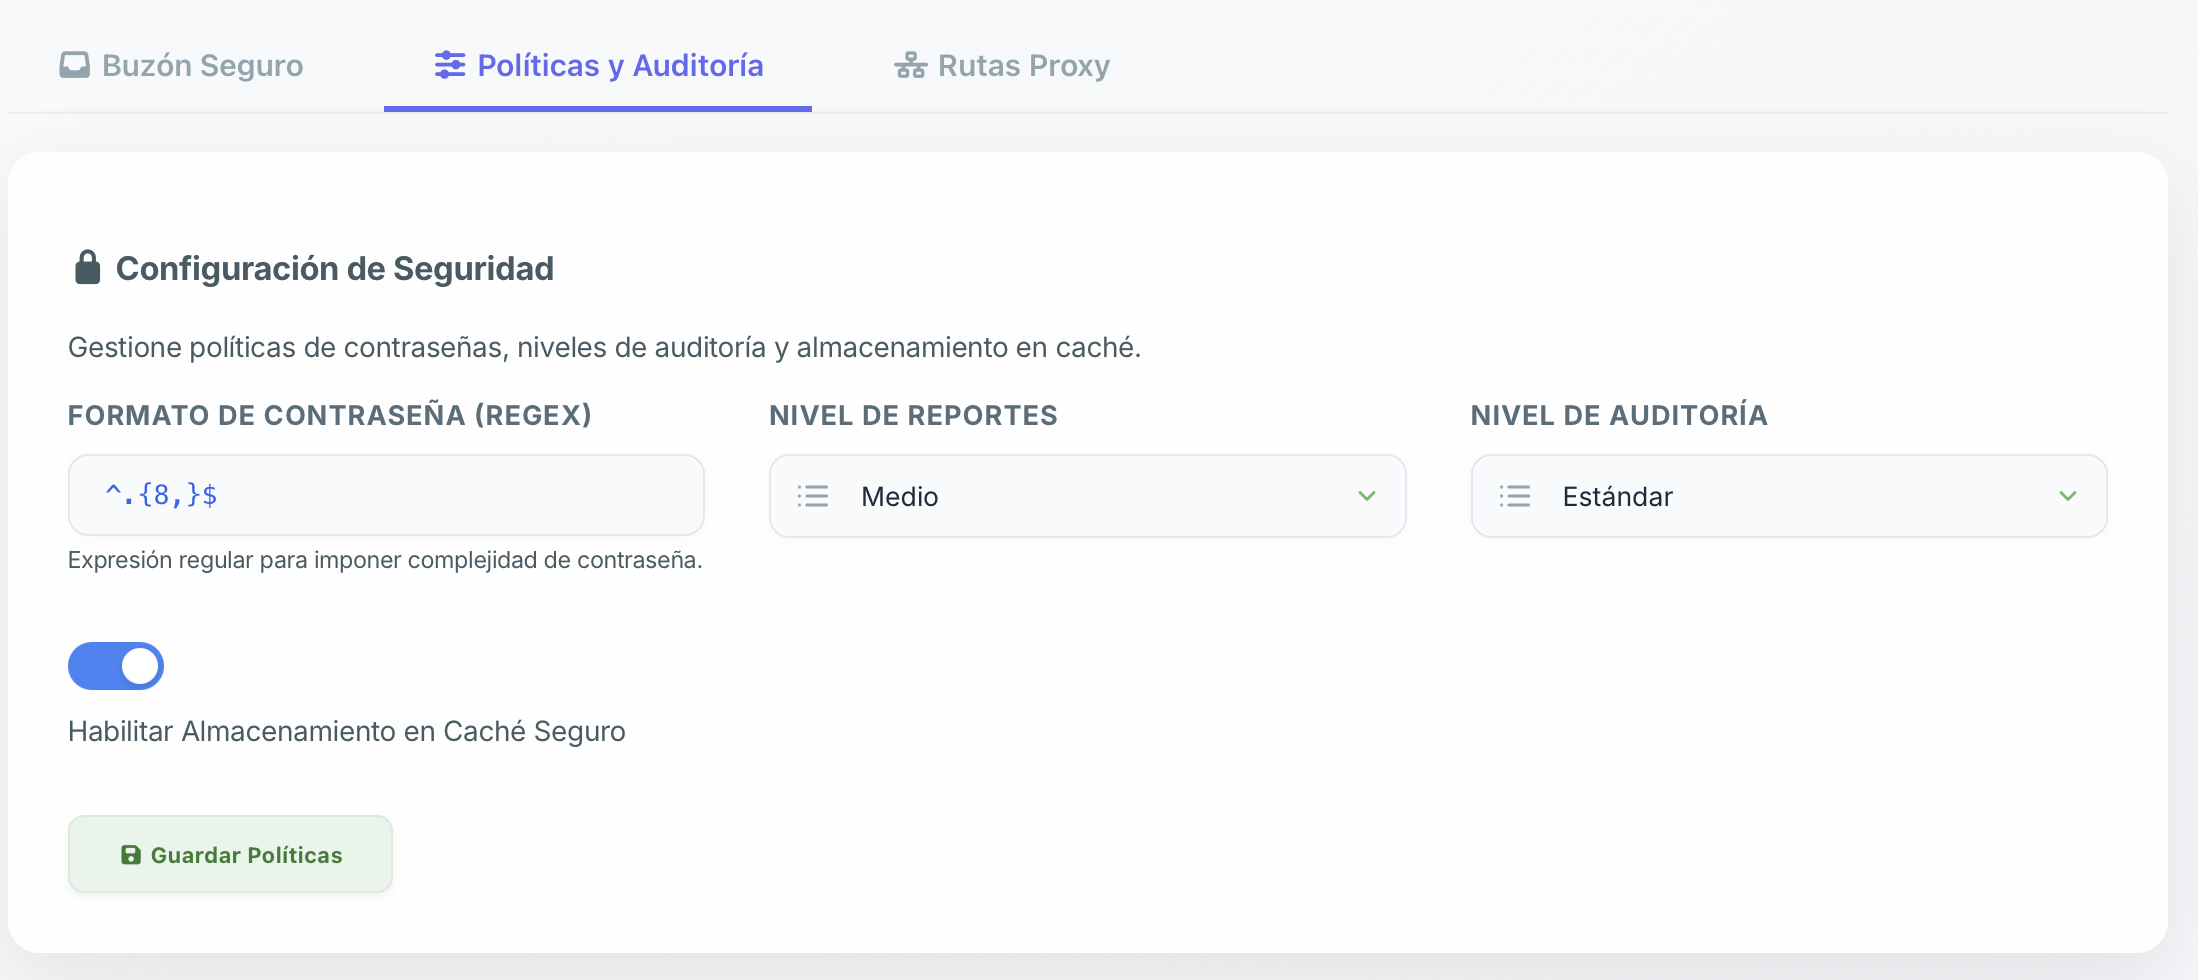
\includegraphics[width=0.95\textwidth]{anexos/8 politica.png}
\caption{Configuracion de politicas de contrasenas}
\label{fig:politicas}
\end{figure}

\subsection{Configuracion de Regex}

\begin{lstlisting}[language=bash, caption={Ejemplos de Regex para Contrasenas}]
# Basica: Minimo 8 caracteres
^(?=.{8,}).*$

# Estandar: 8+ chars, mayuscula, minuscula, numero
^(?=.*[a-z])(?=.*[A-Z])(?=.*\d).{8,}$

# Critica: 12+ chars, mayuscula, minuscula, numero, especial
^(?=.*[a-z])(?=.*[A-Z])(?=.*\d)(?=.*[@$!%*?&]).{12,}$

# Militar: 16+ chars, todos los tipos, sin repetidos
^(?=.*[a-z])(?=.*[A-Z])(?=.*\d)(?=.*[@$!%*?&])(?!.*(.)\1).{16,}$
\end{lstlisting}

\subsection{Algoritmo de Hashing}

Las credenciales nunca se almacenan en texto plano. SDC utiliza Argon2id para el hashing de contrasenas:

\begin{quote}
\textbf{Argon2id}\\
Argon2 es el ganador de la Password Hashing Competition (2015). La variante Argon2id ofrece resistencia a ataques de GPU y ASIC, y proteccion contra ataques de canal lateral.
\end{quote}

\begin{itemize}
    \item Memoria: 64 MB por operacion de hash
    \item Iteraciones: 3 passes
    \item Paralelismo: 4 threads
    \item Sal: 128 bits aleatorios unicos por contrasena
\end{itemize}

\section{Rutas Proxy}
\label{sec:rutas-proxy}

Las rutas proxy definen puntos de acceso seguro para los servicios expuestos por los contenedores.

\begin{figure}[H]
\centering
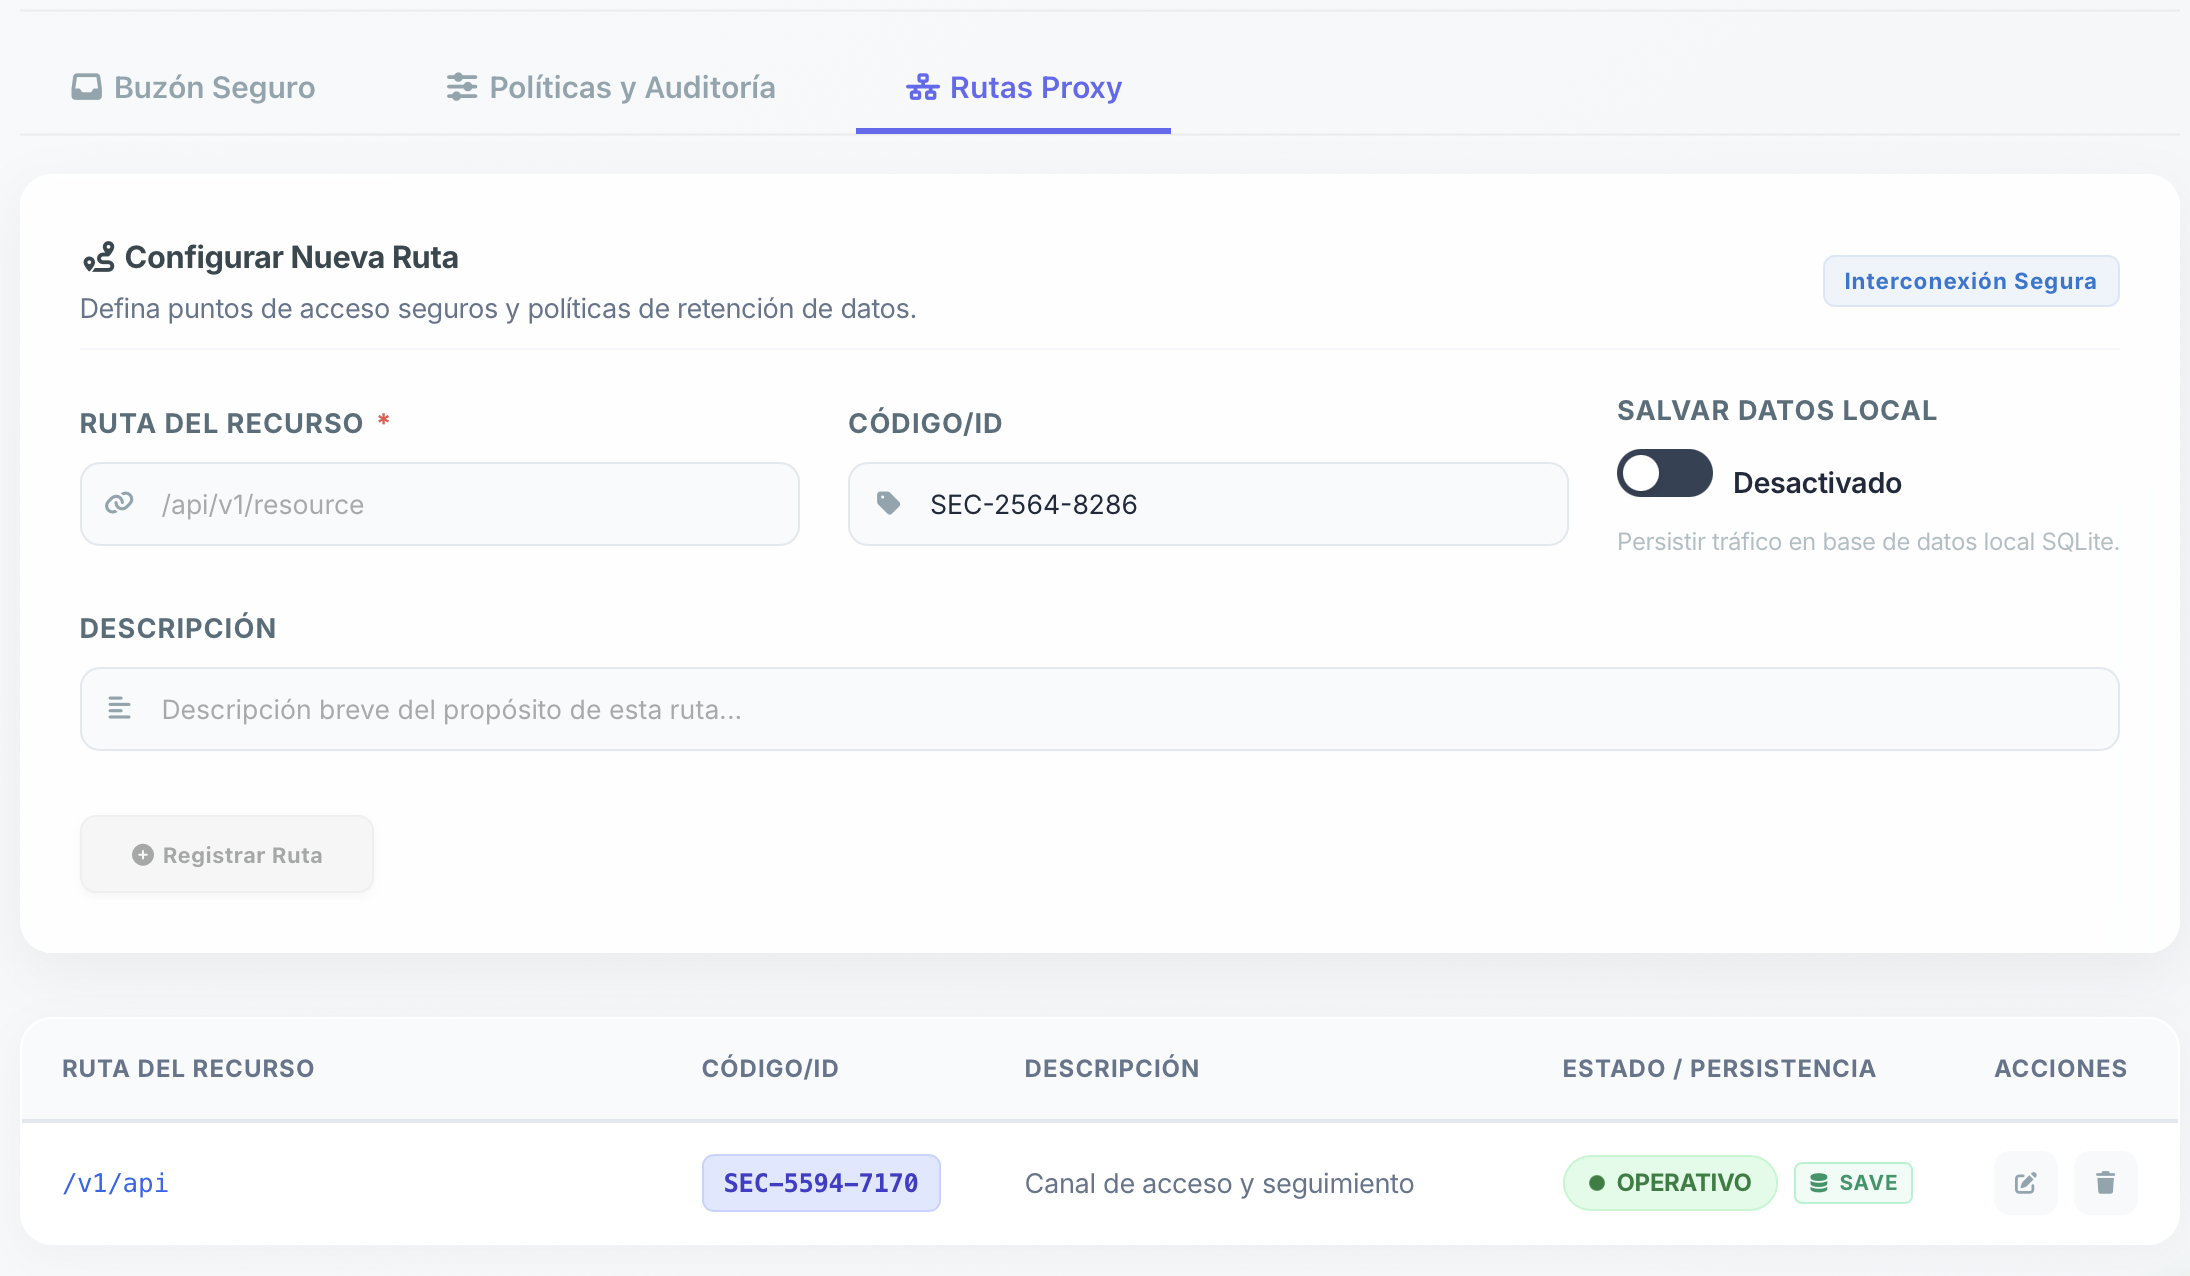
\includegraphics[width=0.95\textwidth]{anexos/9 proxy.png}
\caption{Gestor de rutas proxy}
\label{fig:proxy}
\end{figure}

\subsection{Creacion de Rutas}

Para cada ruta creada (ejemplo: /v1/api), SDC:

\begin{enumerate}[leftmargin=*]
    \item Genera un Codigo ID de Seguridad unico
    \item Configura el enrutamiento interno
    \item Establece politicas de acceso
    \item Opcionalmente, activa persistencia encriptada
\end{enumerate}

\subsection{Codigo ID de Seguridad}

El Codigo ID es un identificador criptografico que:

\begin{itemize}[leftmargin=*]
    \item Vincula la ruta a un Client ID especifico
    \item Incluye timestamp de creacion para expiracion opcional
    \item Se firma con la clave privada del nodo
    \item Se puede revocar individualmente
\end{itemize}

\subsection{Persistencia de Trafico}

\begin{quote}
\textbf{Encriptacion de Datos Persistentes}\\
Cuando la persistencia esta activada, todo el trafico se almacena localmente encriptado con AES-256-GCM. La clave de cifrado se deriva del Client ID mediante HKDF.
\end{quote}

\section{Auditoria y Logs}
\label{sec:auditoria}

SDC mantiene un registro inmutable de todas las operaciones.

\subsection{Niveles de Auditoria}

\begin{table}[H]
\centering
\begin{tabular}{p{3cm}p{4cm}p{6cm}}
\toprule
\textbf{Nivel} & \textbf{Eventos Registrados} & \textbf{Retencion} \\
\midrule
Basico & Inicio/cierre de sesion, errores criticos & 30 dias \\
\midrule
Estandar & Cambios de configuracion, accesos a documentos & 90 dias \\
\midrule
Critico & Todo trafico de red, queries de BD, IPC & 1 ano \\
\bottomrule
\end{tabular}
\caption{Niveles de auditoria y retencion de logs}
\label{tab:niveles-auditoria}
\end{table}

\subsection{Estructura de Logs}

\begin{lstlisting}[language=bash, caption={Formato de Log de Auditoria}]
{
  "timestamp": "2026-03-03T14:32:18.423Z",
  "level": "INFO",
  "client_id": "a1b2c3d4-e5f6...",
  "node_name": "sandra.produccion",
  "event": "DOCUMENT_ACCESS",
  "resource": "/docs/confidencial.pdf",
  "action": "VIEW",
  "result": "SUCCESS",
  "metadata": {
    "ip_source": "192.168.1.100",
    "session_id": "sess-xyz789"
  },
  "hash": "sha256:abc123...",
  "signature": "sig:def456..."
}
\end{lstlisting}

\section{Arquitectura de Defensa en Profundidad}

La seguridad de SDC se organiza en multiples capas:

\begin{enumerate}
    \item \textbf{Perimetro}: Firewall + WSS/TLS 1.3
    \item \textbf{Autenticacion}: Argon2id + MFA
    \item \textbf{Autorizacion}: RBAC + Rutas Proxy
    \item \textbf{Datos}: AES-256-GCM en reposo y transito
    \item \textbf{Auditoria}: Logs inmutables + Firma digital
\end{enumerate}


\part{Seguridad Avanzada}
%======================================================================
% CAPITULO 5: VISOR DE DOCUMENTOS SEGURO
%======================================================================

\chapter{Visor de Documentos Seguro}
\label{ch:visor}

Una de las caracteristicas exclusivas de \sdc{} es el \textbf{Visor Seguro}, que permite visualizar documentos confidenciales sin dejar rastro fisico en el disco duro.

\section{Visor Seguro de SDC}
\label{sec:visor-seguro}

El visor implementa un modelo de seguridad unico: los documentos se desencriptan directamente en la memoria RAM y nunca se escriben en el almacenamiento persistente.

\begin{figure}[H]
\centering
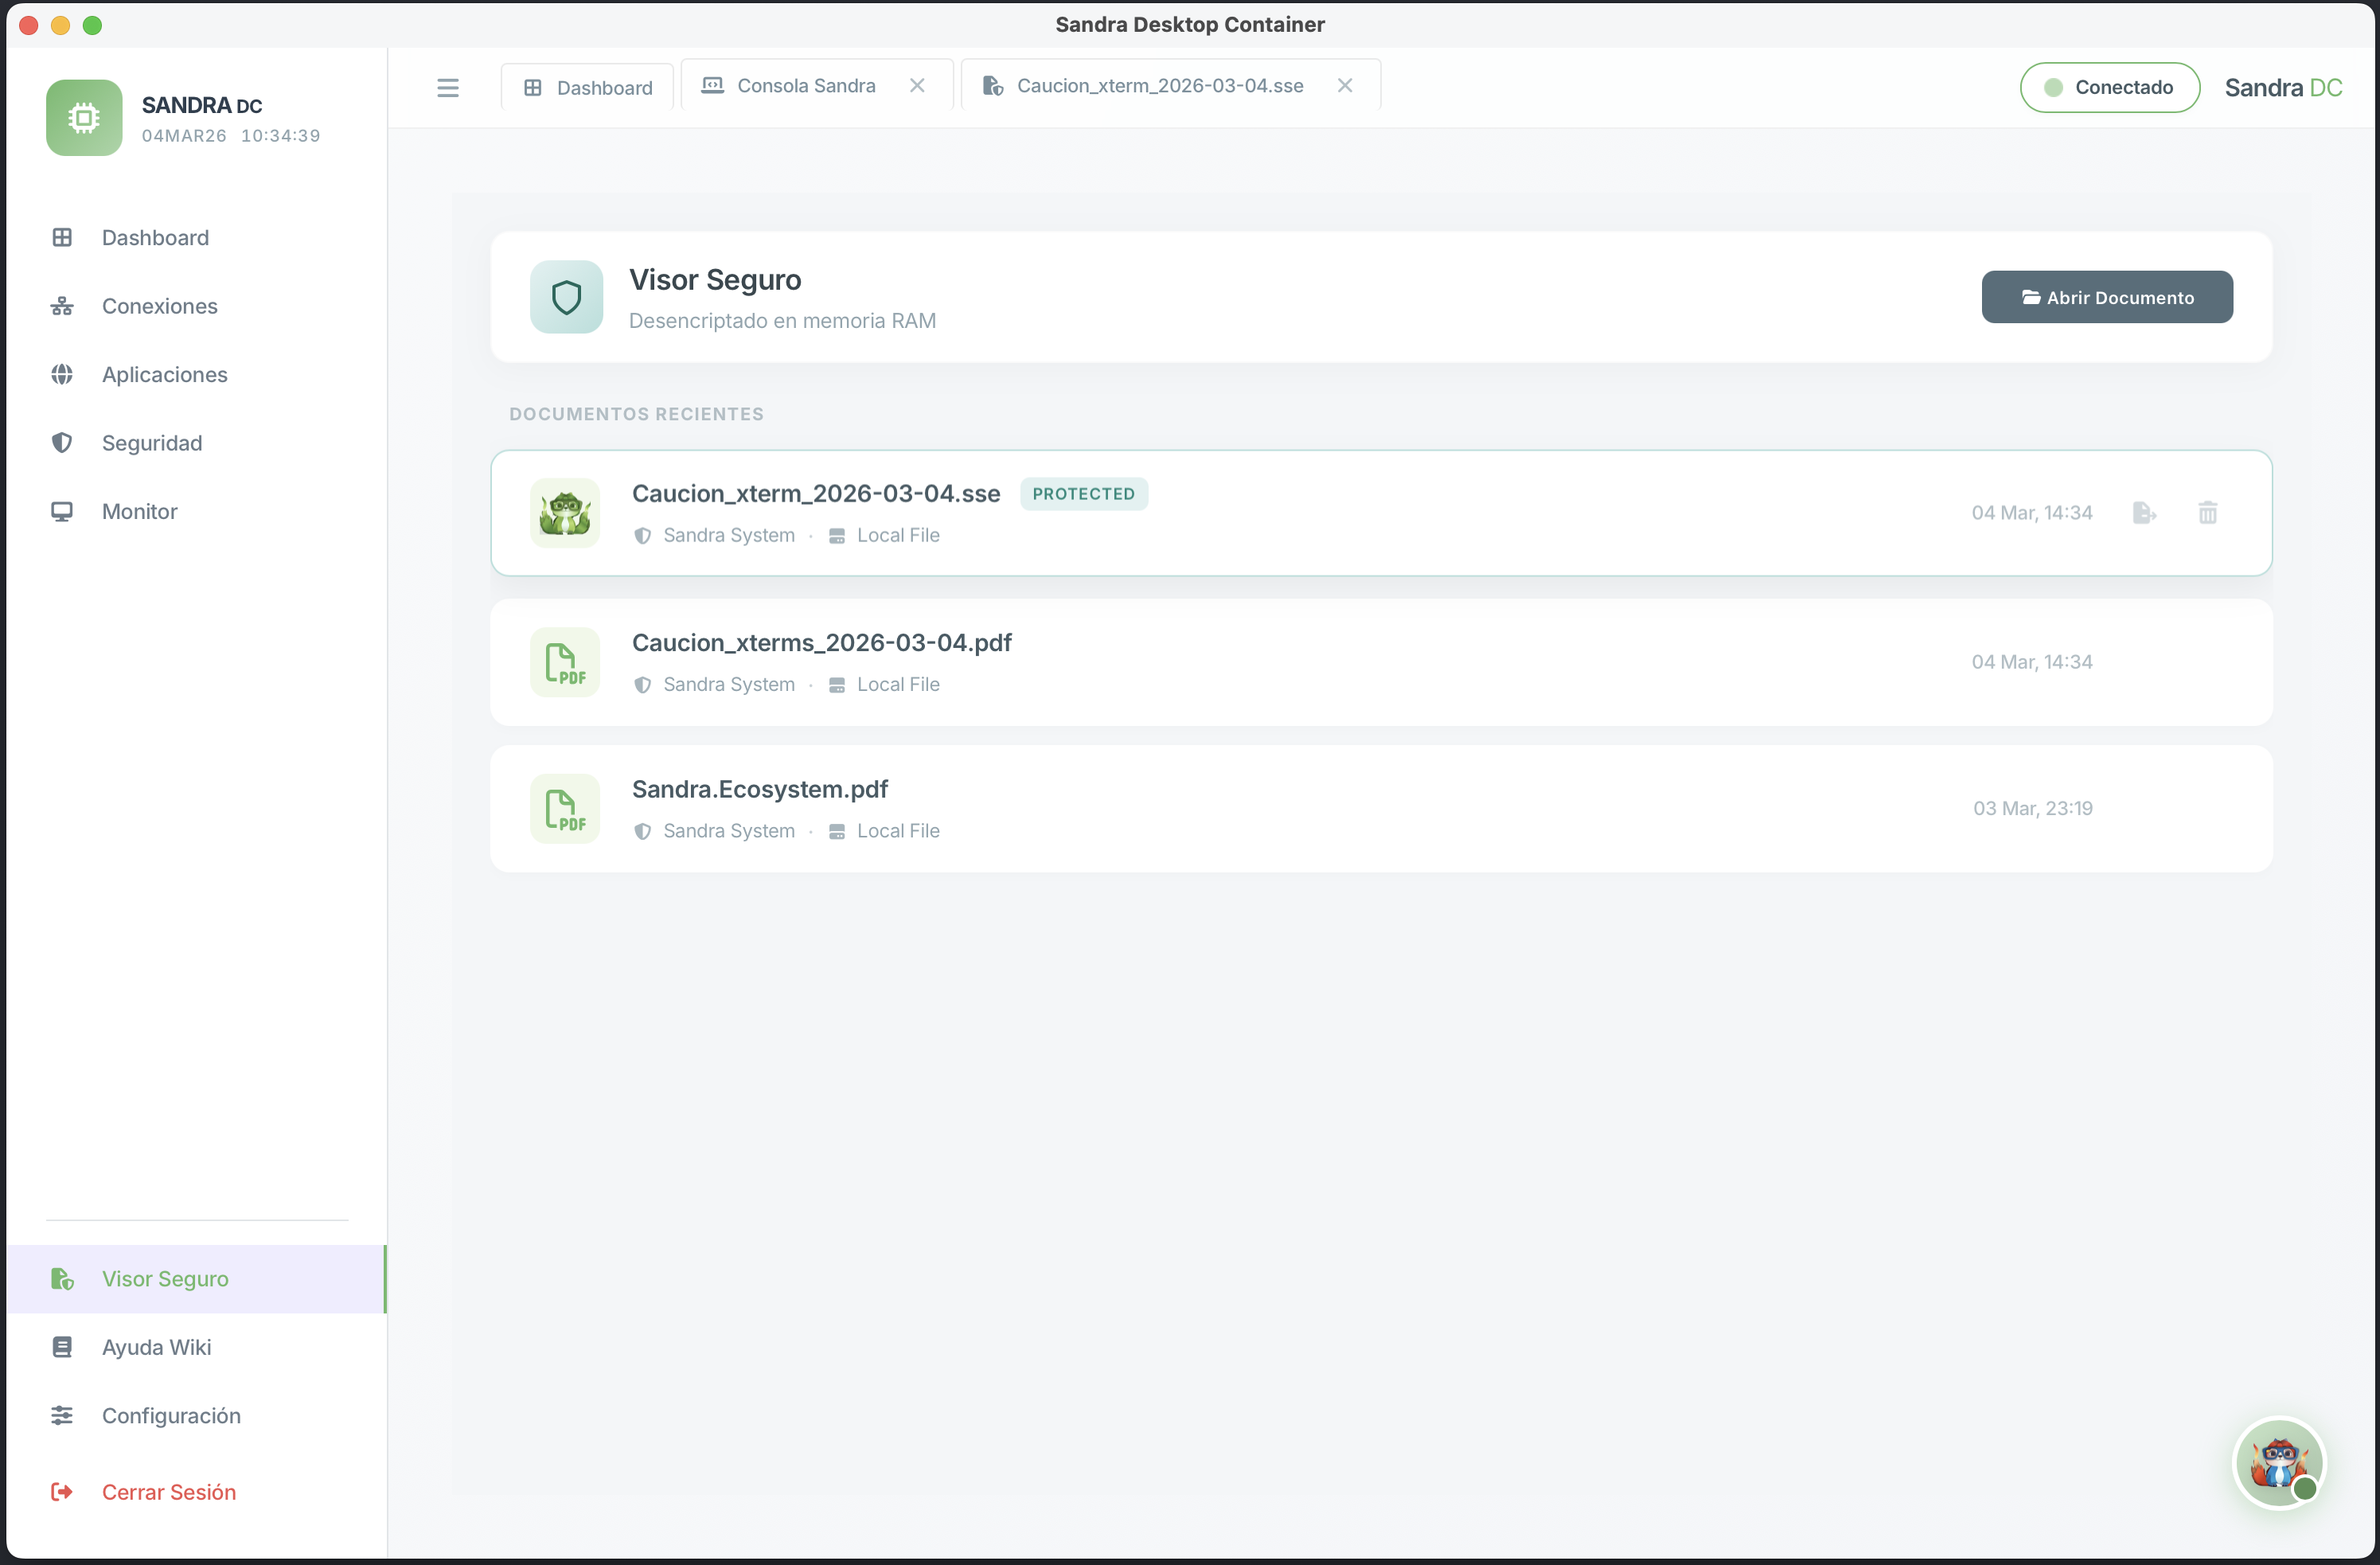
\includegraphics[width=0.95\textwidth]{anexos/11 visor.png}
\caption{Visor seguro de documentos}
\label{fig:visor}
\end{figure}

\subsection{Principio de Operacion}

\begin{enumerate}[leftmargin=*]
    \item El documento encriptado se transfiere desde el servidor origen
    \item Se descifra en tiempo real usando la clave privada del Client ID
    \item El contenido plano se mantiene unicamente en buffers de memoria RAM
    \item Se renderiza en el visor sin crear archivos temporales
    \item Al cerrar, los buffers se sobrescriben con ceros (zero-fill)
\end{enumerate}

\begin{quote}
\textbf{Proteccion Forense}\\
Al cerrar el visor, no queda rastro fisico del archivo en el disco duro. Esto evita la fuga de datos mediante tecnicas de analisis forense digital.
\end{quote}

\section{Formatos Soportados}
\label{sec:formatos}

El visor soporta multiples formatos de documento:

\begin{table}[H]
\centering
\begin{tabular}{p{4cm}p{3cm}p{6cm}}
\toprule
\textbf{Formato} & \textbf{Extension} & \textbf{Caracteristicas} \\
\midrule
PDF & .pdf & Visualizacion nativa con anotaciones \\
\midrule
Imagenes & .png, .jpg, .gif & Zoom, rotacion, filtros \\
\midrule
Documentos Office & .docx, .xlsx & Renderizado simplificado \\
\midrule
Texto Plano & .txt, .md, .json & Sintaxis resaltada \\
\midrule
Codigo Fuente & .rs, .ts, .js & Coloreado por lenguaje \\
\bottomrule
\end{tabular}
\caption{Formatos de documento soportados por el visor}
\label{tab:formatos}
\end{table}

\section{Lista de Documentos}
\label{sec:lista-documentos}

El panel de lista muestra todos los documentos disponibles.

\begin{figure}[H]
\centering
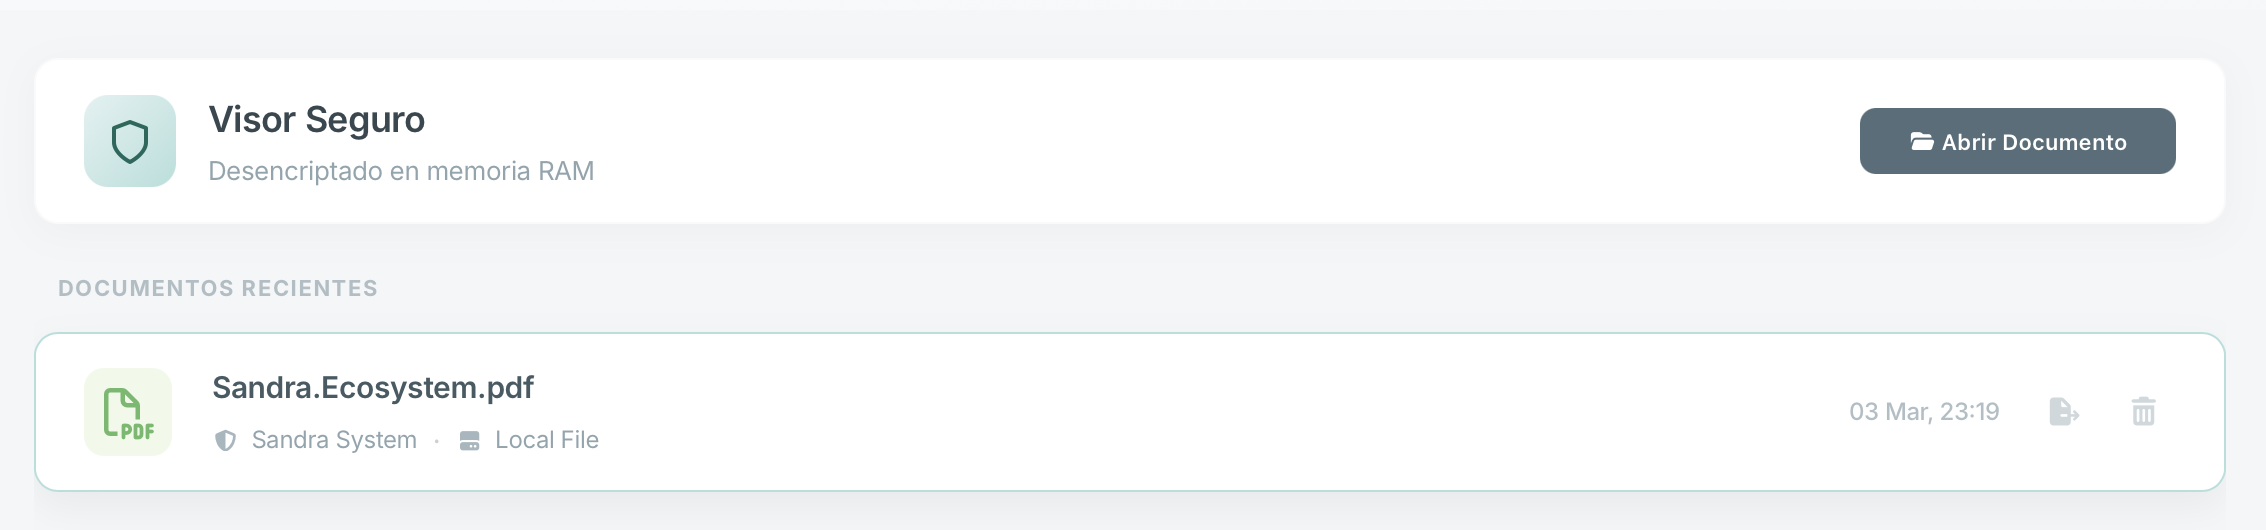
\includegraphics[width=0.95\textwidth]{anexos/13 visor list.png}
\caption{Lista de documentos en el visor}
\label{fig:visor-lista}
\end{figure}

\subsection{Informacion Visualizada}

Para cada documento se muestra:

\begin{itemize}[leftmargin=*]
    \item Nombre del archivo
    \item Tamanio en formato legible
    \item Fecha de ultima modificacion
    \item Estado de encriptacion (Verde: Encriptado)
    \item Propietario o autor
    \item Etiquetas de clasificacion
\end{itemize}

\section{Encriptacion de Documentos}
\label{sec:encriptacion}

\begin{figure}[H]
\centering
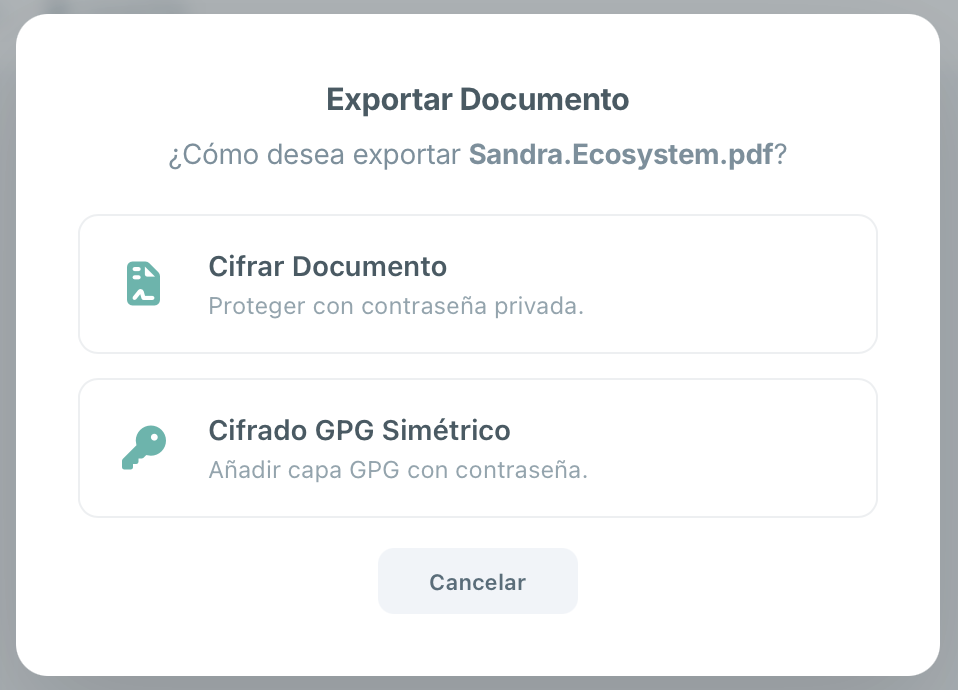
\includegraphics[width=0.95\textwidth]{anexos/14 visor encriptado.png}
\caption{Estado de documento encriptado}
\label{fig:visor-encriptado}
\end{figure}

\subsection{Esquema de Encriptacion}

SDC utiliza SSE (Sandra Secure Encryption), un esquema hibrido:

\begin{enumerate}
    \item \textbf{Cifrado Simetrico}: AES-256-GCM para el contenido
    \item \textbf{Cifrado Asimetrico}: RSA-4096 para proteger la clave AES
    \item \textbf{Clave de Sesion}: Generada aleatoriamente para cada documento
    \item \textbf{Derivacion}: HKDF-SHA256 para claves derivadas
\end{enumerate}

\subsection{Proceso de Cifrado}

\begin{enumerate}[leftmargin=*]
    \item Generar clave AES-256 aleatoria (32 bytes)
    \item Cifrar el documento con AES-256-GCM
    \item Cifrar la clave AES con la clave publica RSA del destinatario
    \item Empaquetar: documento cifrado + clave cifrada + metadatos
    \item Firmar digitalmente el paquete con la clave privada del emisor
\end{enumerate}

\section{Previsualizacion de Archivos}
\label{sec:preview}

El modo de previsualizacion permite obtener una vista rapida sin cargar el documento completo.

\begin{figure}[H]
\centering
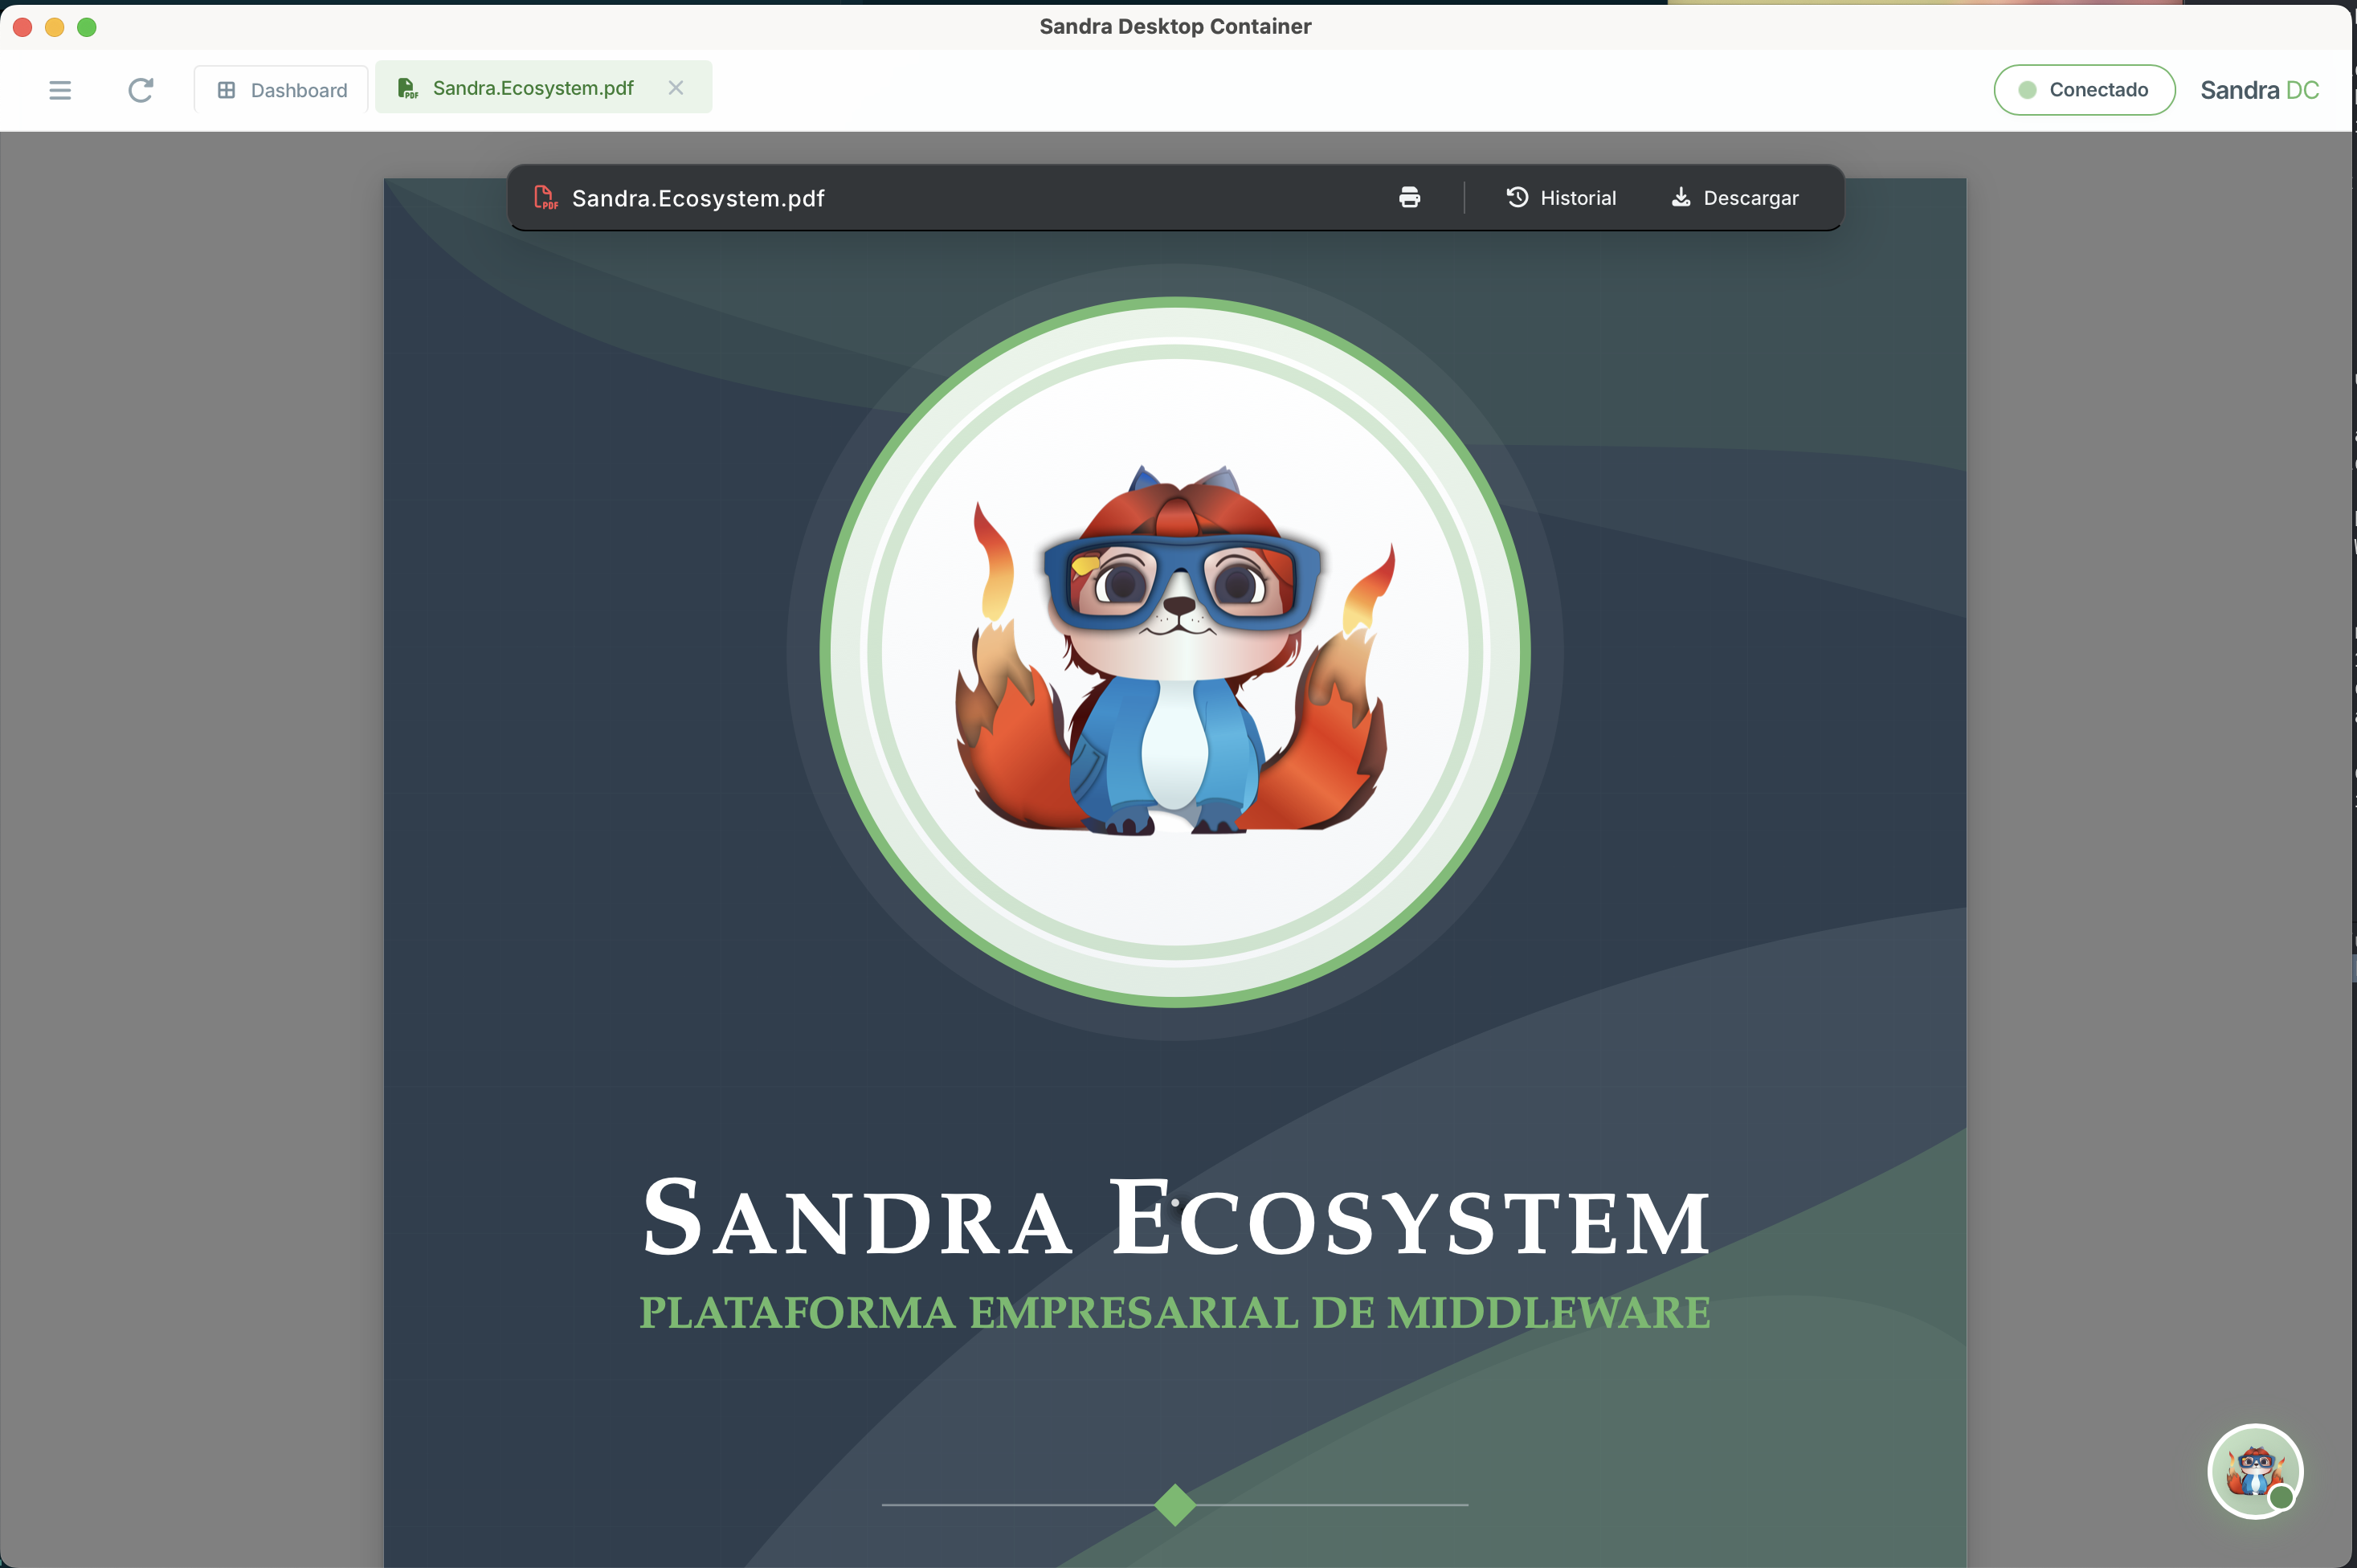
\includegraphics[width=0.95\textwidth]{anexos/12 preview-file.png}
\caption{Previsualizacion de archivo}
\label{fig:preview}
\end{figure}

\section{Configurador del Visor}
\label{sec:configurador}

El configurador permite ajustar el comportamiento del visor.

\begin{figure}[H]
\centering
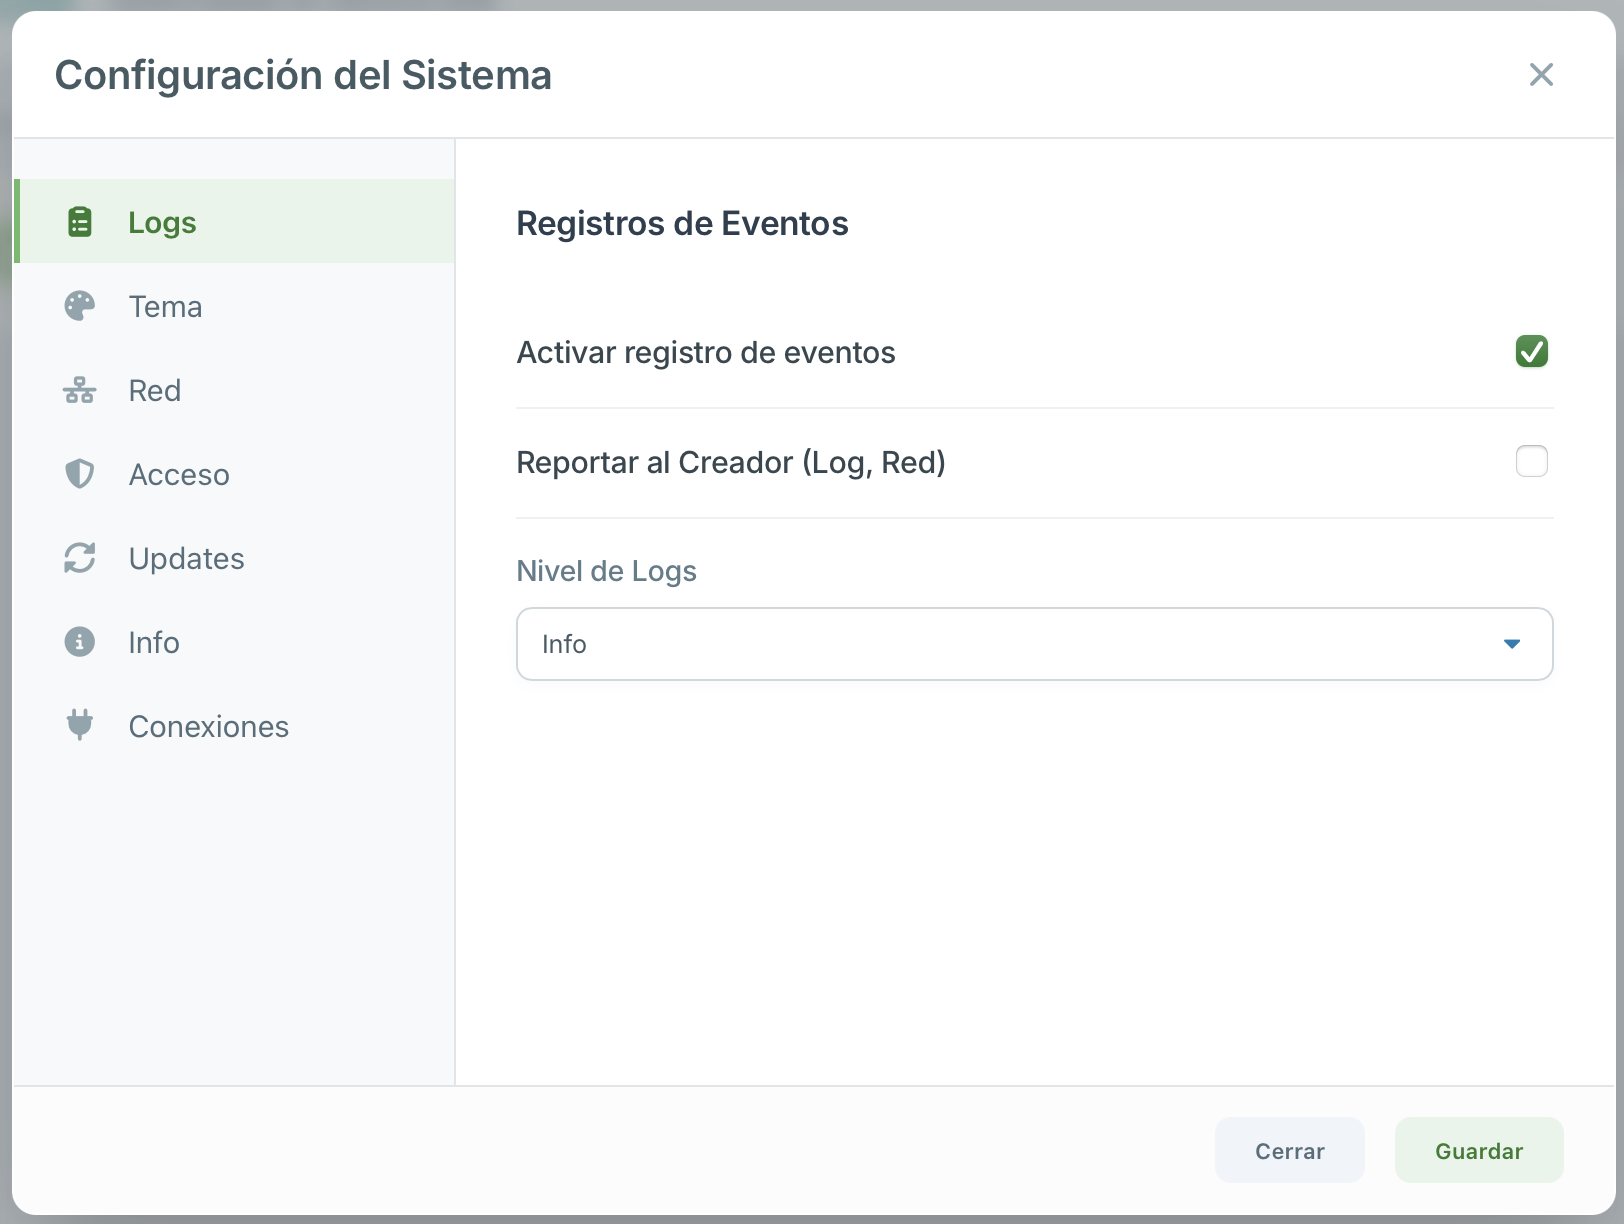
\includegraphics[width=0.95\textwidth]{anexos/15 configurador.png}
\caption{Configurador del visor de documentos}
\label{fig:configurador}
\end{figure}

\subsection{Opciones de Configuracion}

\begin{table}[H]
\centering
\begin{tabular}{p{5cm}p{3cm}p{5cm}}
\toprule
\textbf{Opcion} & \textbf{Valores} & \textbf{Efecto} \\
\midrule
Auto-cierre por inactividad & 1-60 minutos & Cierra documento tras inactividad \\
\midrule
Prevenir capturas de pantalla & Si / No & Bloquea PrintScreen y grabacion \\
\midrule
Marcas de agua dinamicas & Si / No & Superpone ID de sesion en vista \\
\midrule
Nivel de zoom por defecto & 50-200 por ciento & Ajuste inicial de visualizacion \\
\bottomrule
\end{tabular}
\caption{Opciones de configuracion del visor}
\label{tab:config-visor}
\end{table}

\begin{quote}
\textbf{Marcas de Agua Dinamicas}\\
Cuando estan activadas, el visor superpone una marca de agua semitransparente que incluye: Client ID del nodo, timestamp de apertura, y nombre de usuario.
\end{quote}

\section{Flujo de Seguridad del Visor}

El proceso de seguridad del visor sigue estos pasos:

\begin{enumerate}
    \item \textbf{Solicitud de Apertura}: El usuario solicita abrir un documento
    \item \textbf{Autorizacion}: Verificacion de permisos y credenciales
    \item \textbf{Descifrado en RAM}: El documento se descifra en memoria volatil
    \item \textbf{Renderizado}: Visualizacion del contenido descifrado
    \item \textbf{Visualizacion Activa}: El usuario interactua con el documento
    \item \textbf{Cierre}: Al cerrar, se aplica zero-fill a la memoria
    \item \textbf{Registro de Auditoria}: Se registra el evento de acceso
\end{enumerate}

\section{Mejores Practicas}

\begin{enumerate}[leftmargin=*]
    \item Cierra siempre el visor cuando termines de trabajar con documentos sensibles
    \item Habilita el auto-cierre por inactividad (recomendado: 5 minutos)
    \item Usa marcas de agua en entornos compartidos
    \item Bloquea capturas de pantalla para documentos altamente confidenciales
    \item Verifica el hash antes de abrir documentos descargados
\end{enumerate}

\begin{quote}
\textbf{Responsabilidad del Usuario}\\
Aunque el visor proporciona proteccion tecnica robusta, la seguridad final depende del comportamiento del usuario: no fotografiar la pantalla con dispositivos externos, no transcribir informacion sensible a otros medios, cerrar sesion al alejarse del equipo.
\end{quote}


\part{Inteligencia Artificial}
%======================================================================
% CAPITULO 6: CHAT DE SANDRA AI
%======================================================================

\chapter{Chat de Sandra AI}
\label{ch:chat}

\sandraai{} no solo es un asistente de comandos, sino una interfaz conversacional completa que permite interactuar con el ecosistema SDC de forma natural e intuitiva. Este capitulo describe la interfaz de chat y sus capacidades avanzadas.

\section{Interfaz de Conversacion}
\label{sec:interfaz-chat}

El chat de Sandra AI proporciona un espacio de dialogo continuo donde los usuarios pueden realizar consultas, ejecutar comandos y recibir asistencia contextual.

\begin{figure}[H]
\centering
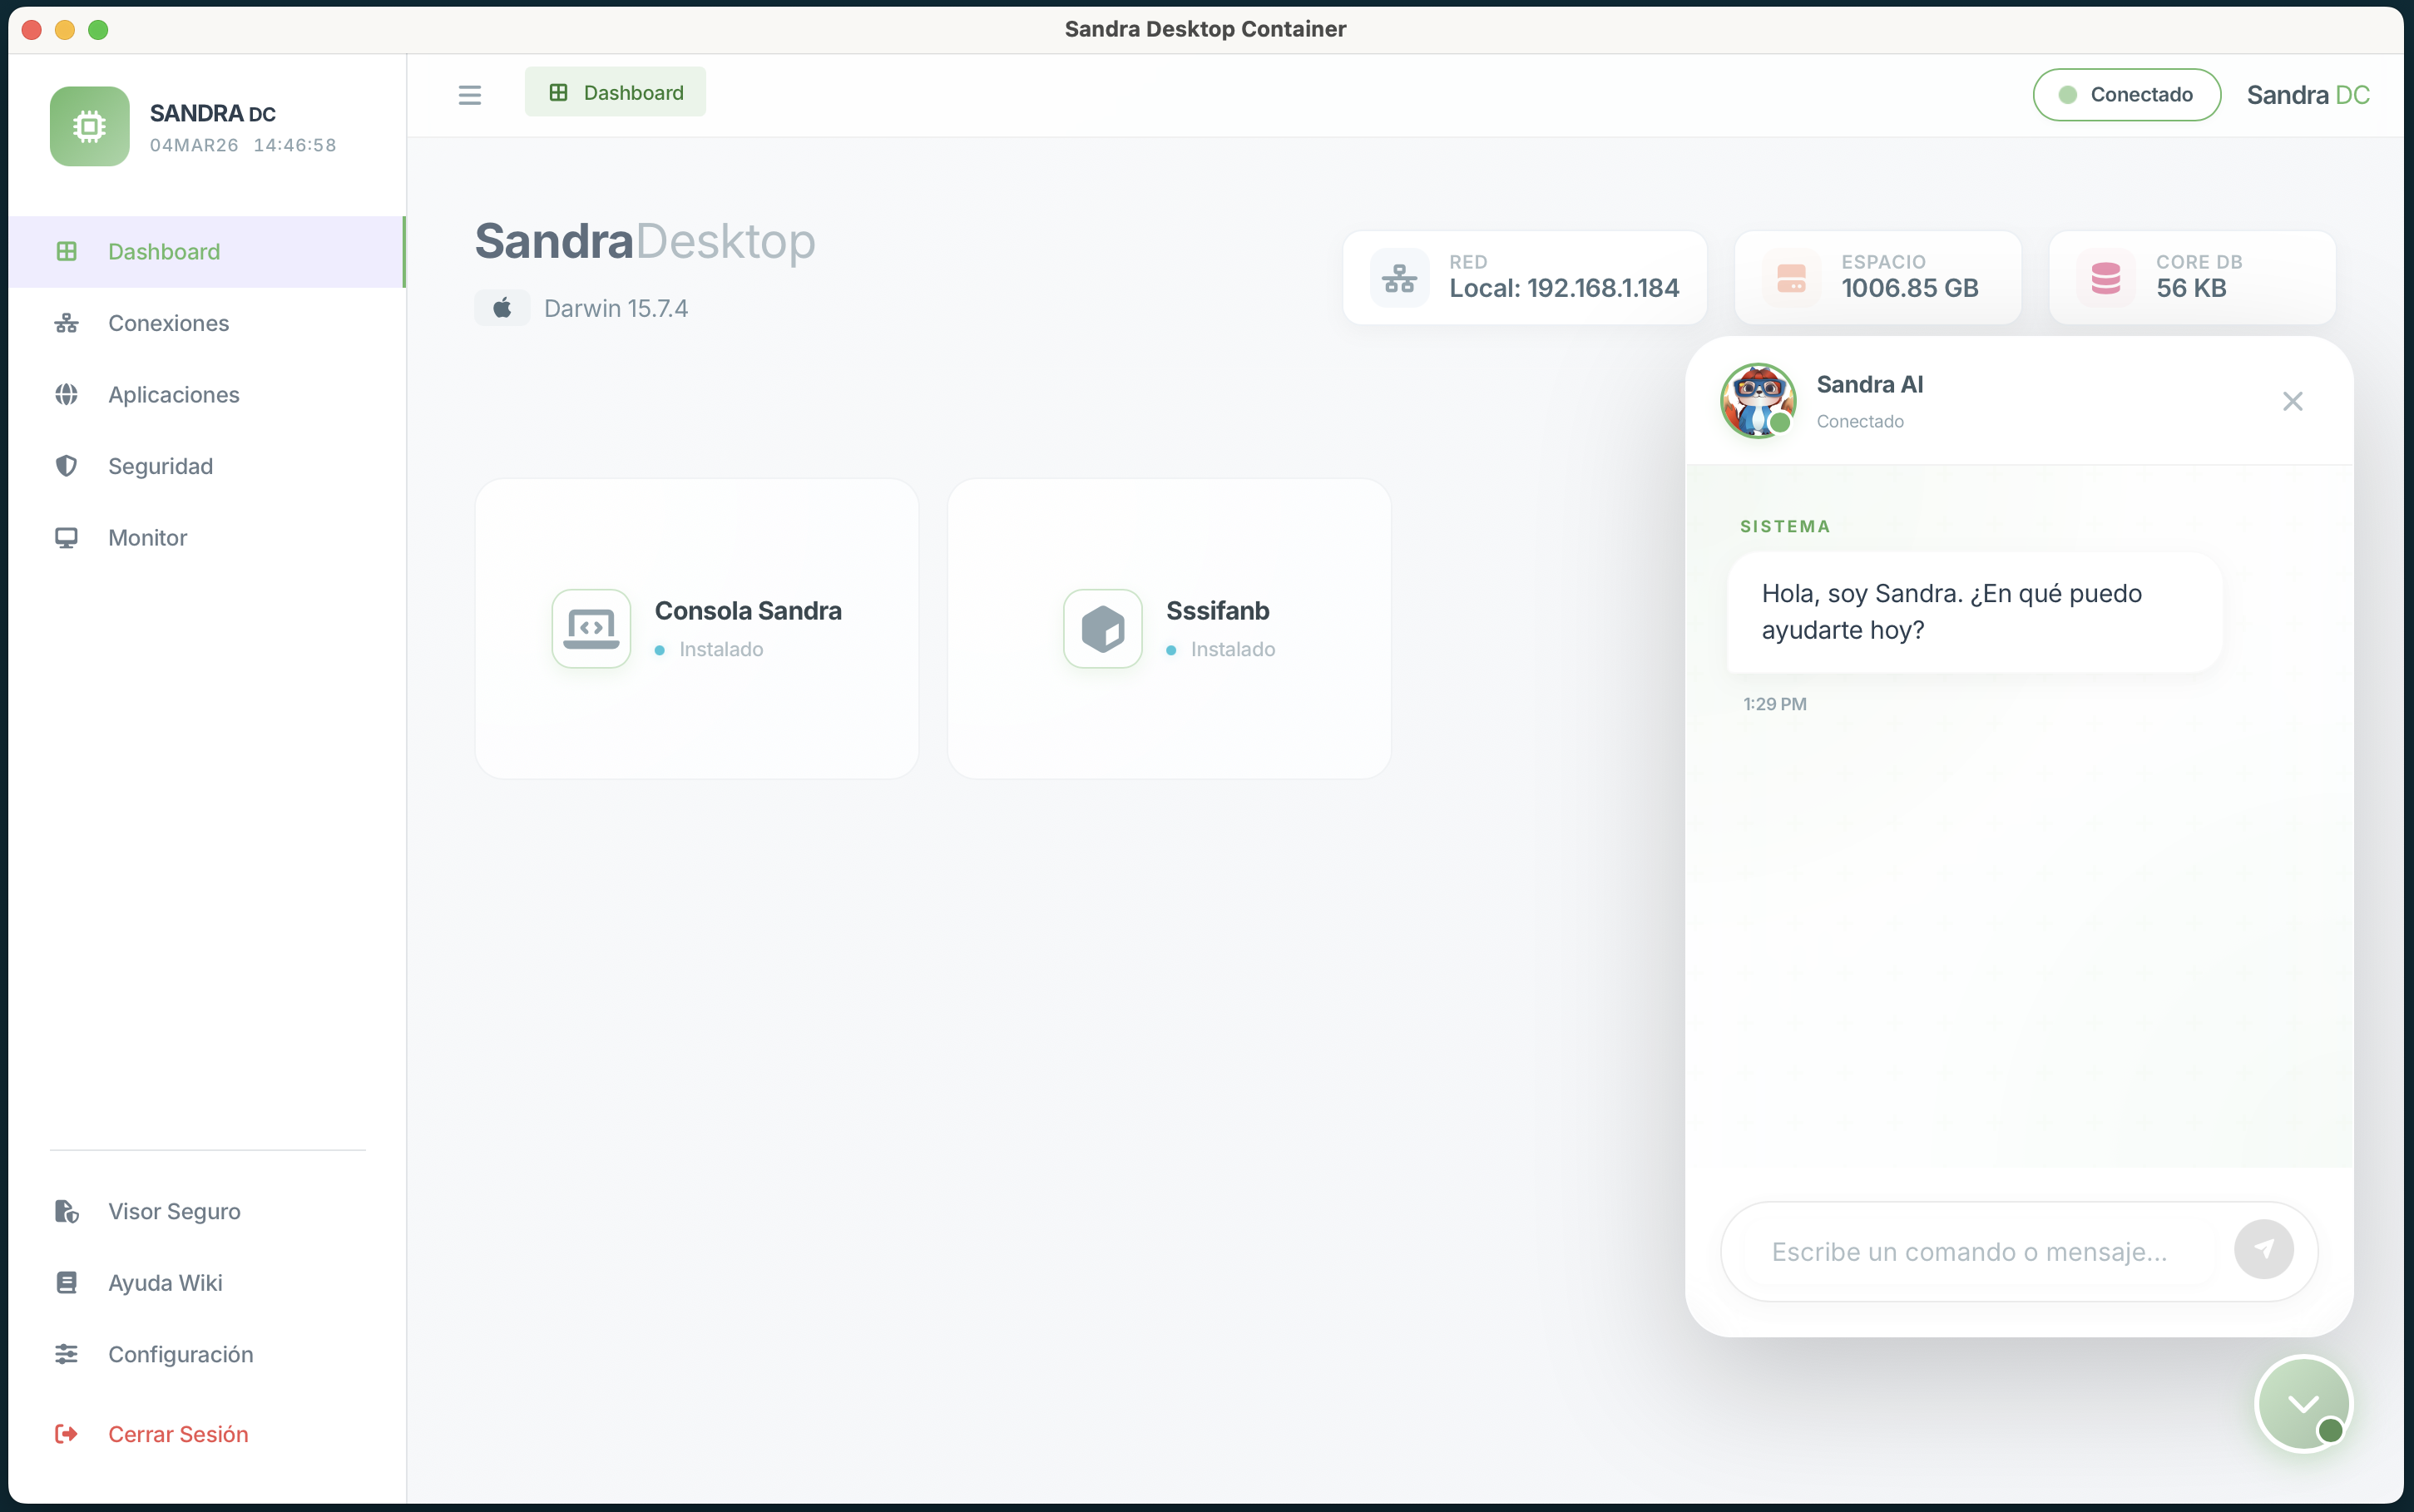
\includegraphics[width=0.95\textwidth]{anexos/chat.png}
\caption{Interfaz de chat de Sandra AI}
\label{fig:chat}
\end{figure}

\subsection{Componentes de la Interfaz}

La interfaz de chat consta de los siguientes elementos:

\begin{itemize}[leftmargin=*]
    \item \textbf{Area de Mensajes}: Historial completo de la conversacion
    \item \textbf{Campo de Entrada}: Donde el usuario escribe sus consultas
    \item \textbf{Sugerencias Contextuales}: Comandos rapidos basados en el contexto actual
    \item \textbf{Indicador de Estado}: Muestra cuando Sandra esta procesando una respuesta
    \item \textbf{Botones de Accion}: Accesos directos a funciones frecuentes
\end{itemize}

\subsection{Historial de Conversaciones}

Sandra AI mantiene un historial persistente de conversaciones que incluye:

\begin{itemize}[leftmargin=*]
    \item \textbf{Contexto de Sesion}: Recuerda el tema de la conversacion actual
    \item \textbf{Referencias Cruzadas}: Puede referirse a elementos mencionados anteriormente
    \item \textbf{Aprendizaje Adaptativo}: Mejora las respuestas basandose en interacciones previas
    \item \textbf{Busqueda en Historial}: Permite recuperar informacion de conversaciones pasadas
\end{itemize}

\begin{quote}
\textbf{Privacidad del Historial}\\
El historial de conversaciones se almacena localmente en la base de datos cifrada de SDC. No se transmite a servidores externos y puede borrarse completamente por el usuario en cualquier momento.
\end{quote}

\section{Comandos y Consultas}
\label{sec:comandos-chat}

Sandra AI procesa diferentes tipos de entrada, desde preguntas simples hasta comandos complejos.

\subsection{Consultas de Informacion}

El usuario puede realizar preguntas sobre el sistema y recibir respuestas detalladas:

\begin{table}[H]
\centering
\begin{tabular}{p{8cm}p{6cm}}
\toprule
\textbf{Consulta} & \textbf{Respuesta Esperada} \\
\midrule
Cual es el estado del sistema? & Metricas generales y estado de servicios \\
\midrule
Cuanto espacio libre tengo en disco? & Informacion de almacenamiento disponible \\
\midrule
Muestrame los logs de conexiones recientes & Visor de logs filtrado por conexiones \\
\midrule
Que aplicaciones tengo instaladas? & Lista completa de apps desplegadas \\
\midrule
Explicame que es una ruta proxy & Definicion y funcionamiento de proxies \\
\bottomrule
\end{tabular}
\caption{Ejemplos de consultas informativas}
\label{tab:consultas-chat}
\end{table}

\subsection{Comandos Operativos}

Sandra puede ejecutar acciones directamente desde el chat:

\begin{table}[H]
\centering
\begin{tabular}{p{7cm}p{7cm}}
\toprule
\textbf{Comando} & \textbf{Accion Ejecutada} \\
\midrule
Crear nueva conexion al servidor produccion & Abre formulario de nueva conexion pre-cargado \\
\midrule
Abrir la aplicacion de correo & Lanza la app de correo configurada \\
\midrule
Desactivar el proxy para la app de testing & Cambia modo de navegacion a libre \\
\midrule
Generar reporte de auditoria de la ultima semana & Crea y exporta reporte PDF \\
\midrule
Limpiar los logs de sesion & Elimina logs temporales de la sesion actual \\
\bottomrule
\end{tabular}
\caption{Comandos operativos via chat}
\label{tab:comandos-operativos}
\end{table}

\subsection{Asistencia Contextual}

Sandra proporciona ayuda adaptada al contexto actual del usuario:

\begin{table}[H]
\centering
\begin{tabular}{p{4cm}p{8cm}}
\toprule
\textbf{Contexto} & \textbf{Asistencia Proporcionada} \\
\midrule
En Dashboard & Sugerencias sobre metricas y alertas \\
\midrule
En Visor de Docs & Ayuda sobre permisos y encriptacion \\
\midrule
Configurando App & Guia paso a paso del formulario \\
\midrule
Error de Conexion & Diagnostico y solucion de problemas \\
\bottomrule
\end{tabular}
\caption{Asistencia contextual de Sandra AI}
\label{tab:asistencia-contextual}
\end{table}

\section{Funciones Avanzadas}
\label{sec:funciones-avanzadas}

\subsection{Procesamiento de Lenguaje Natural}

Sandra AI utiliza tecnicas de NLP para entender consultas formuladas de forma natural:

\begin{itemize}[leftmargin=*]
    \item \textbf{Sinonimos}: Reconoce diferentes formas de expresar la misma intencion
    \item \textbf{Correccion Ortografica}: Corrige errores tipograficos automaticamente
    \item \textbf{Interpretacion Contextual}: Entiende referencias a elementos mencionados anteriormente
    \item \textbf{Multilenguaje}: Soporta consultas en espanol e ingles
\end{itemize}

\begin{quote}
\textbf{Ejemplo de Comprension Contextual}\\
Usuario: Abre la primera aplicacion de la lista\\
Sandra: Entiende que se refiere a la primera app mostrada en el dashboard actual y la abre.
\end{quote}

\subsection{Automatizacion de Tareas}

El chat permite crear secuencias de comandos automatizadas:

\begin{quote}
\textbf{Ejemplo de Automatizacion}\\
Usuario: Crea un backup diario de la base de datos\\
Sandra: He configurado una tarea programada para backup diario a las 02:00 AM. Se guardaran en /backups/automaticos/ y se mantendran las ultimas 30 copias.
\end{quote}

\subsection{Integracion con el Sistema}

Sandra AI esta profundamente integrada con todas las funciones de SDC:

\begin{itemize}[leftmargin=*]
    \item \textbf{Control de Aplicaciones}: Iniciar, detener, configurar apps
    \item \textbf{Gestion de Conexiones}: Crear, editar, monitorear conexiones
    \item \textbf{Seguridad}: Configurar politicas, revisar logs de auditoria
    \item \textbf{Monitorizacion}: Consultar metricas en tiempo real
    \item \textbf{Documentos}: Buscar, abrir, compartir archivos del visor
\end{itemize}

\section{Mejores Practicas}
\label{sec:mejores-practicas-chat}

\begin{enumerate}[leftmargin=*]
    \item \textbf{Sean Especificos}: Cuanta mas informacion proporciones, mejor sera la respuesta
    \item \textbf{Usa Contexto}: Puedes referirte a elementos mencionados anteriormente sin repetirlos
    \item \textbf{Confirma Acciones Criticas}: Para operaciones importantes, Sandra pedira confirmacion
    \item \textbf{Revisa Sugerencias}: Las sugerencias contextuales pueden ahorrar tiempo
    \item \textbf{Guarda Conversaciones Utiles}: Puedes exportar dialogos importantes para referencia futura
\end{enumerate}

\begin{quote}
\textbf{Limitaciones}\\
Aunque Sandra AI es poderosa, tiene limitaciones:
\begin{itemize}
    \item No puede modificar configuraciones de seguridad criticas sin autorizacion
    \item No ejecuta comandos que comprometan la integridad del sistema
    \item No comparte informacion fuera del entorno SDC
    \item Requiere confirmacion para acciones destructivas (eliminar, borrar)
\end{itemize}
\end{quote}

\section{Solucion de Problemas}
\label{sec:solucion-problemas-chat}

\begin{table}[H]
\centering
\begin{tabular}{p{5cm}p{7cm}}
\toprule
\textbf{Problema} & \textbf{Solucion} \\
\midrule
Sandra no entiende mi consulta & Reformula la pregunta con terminos mas tecnicos \\
\midrule
Respuesta irrelevante & Proporciona mas contexto sobre lo que necesitas \\
\midrule
Comando no ejecutado & Verifica que tienes permisos suficientes \\
\midrule
Historial muy largo & Usa el comando limpiar chat para reiniciar \\
\bottomrule
\end{tabular}
\caption{Solucion de problemas comunes en el chat}
\label{tab:problemas-chat}
\end{table}


\part{Configuración Avanzada}
%======================================================================
% CAPITULO 7: CONFIGURACION AVANZADA
%======================================================================

\chapter{Configuracion Avanzada}
\label{ch:configuracion}

Este capitulo describe las opciones de configuracion avanzada de \sdc{}, incluyendo personalizacion visual, ajustes de red, control de acceso y gestion de actualizaciones.

\section{Temas Visuales}
\label{sec:temas}

SDC ofrece multiples temas visuales para adaptarse a las preferencias del usuario y condiciones de uso.

\begin{figure}[H]
\centering
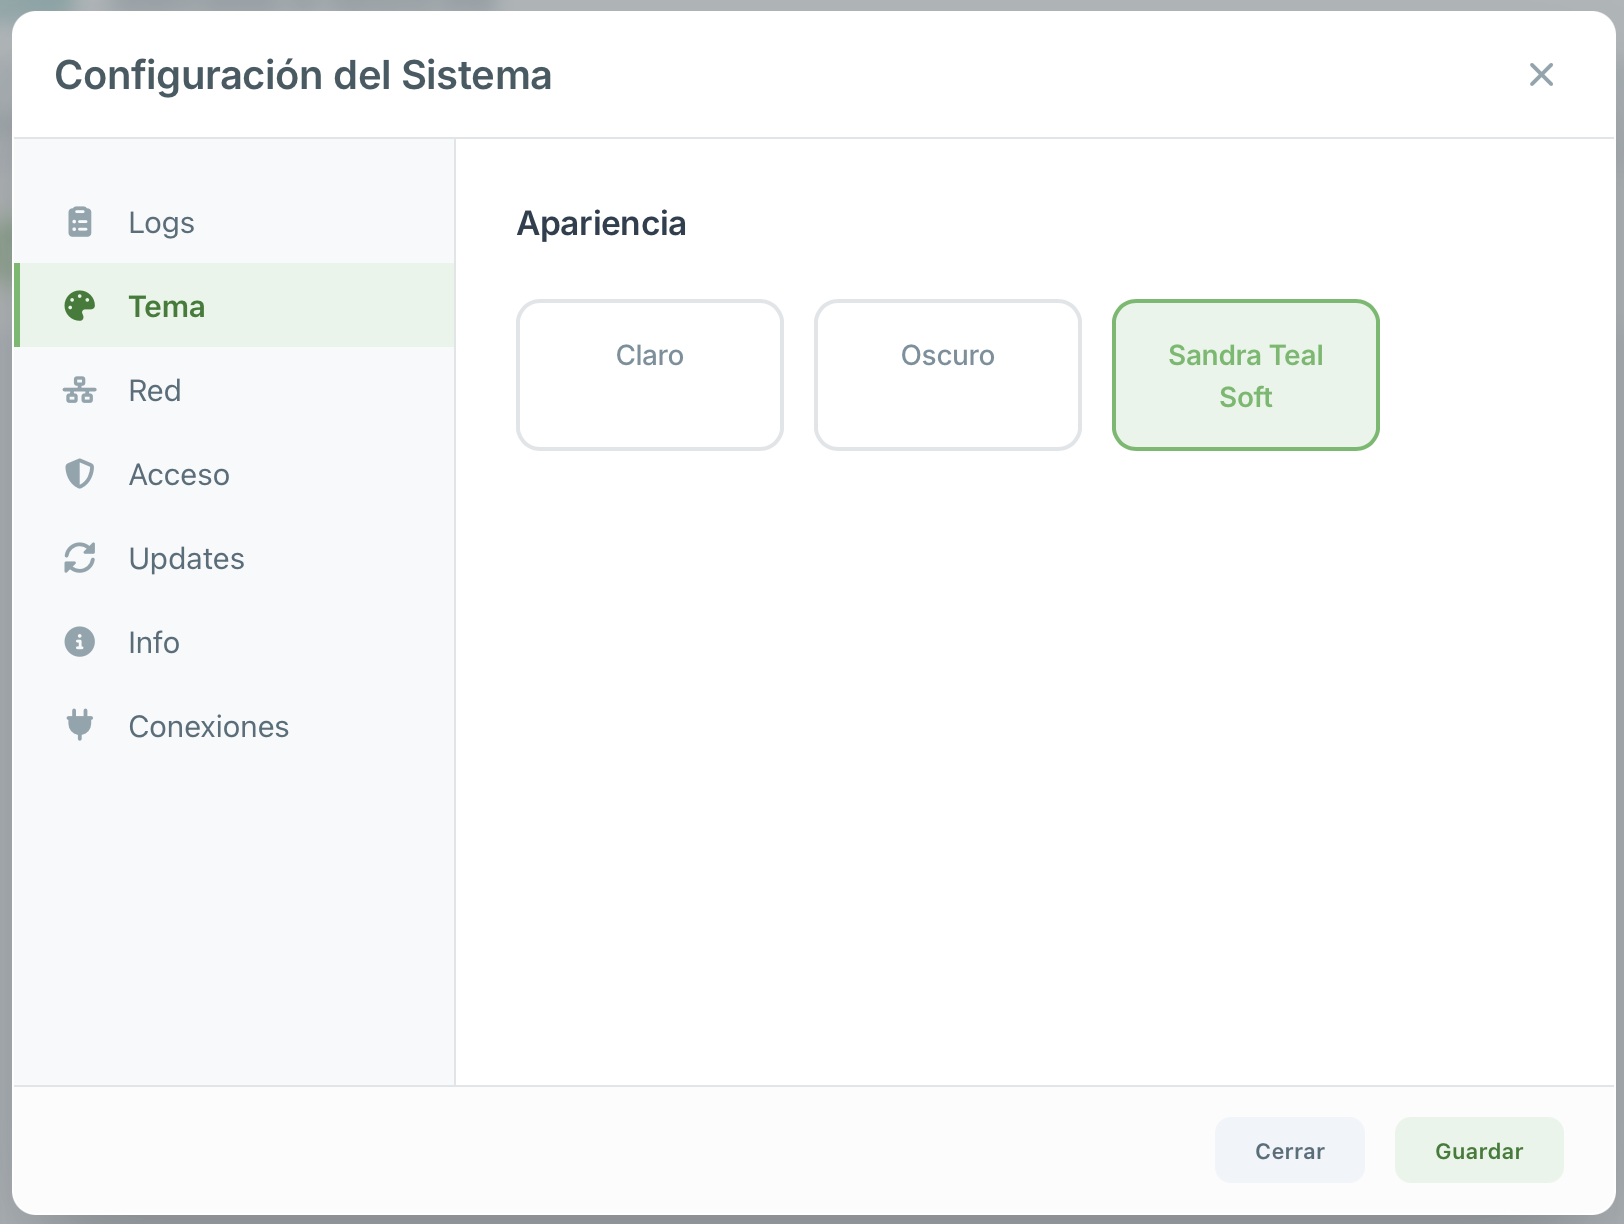
\includegraphics[width=0.95\textwidth]{anexos/17 temas.png}
\caption{Selector de temas visuales}
\label{fig:temas}
\end{figure}

\subsection{Temas Disponibles}

\begin{table}[H]
\centering
\begin{tabular}{p{3.5cm}p{4cm}p{5.5cm}}
\toprule
\textbf{Tema} & \textbf{Caracteristicas} & \textbf{Mejor Para} \\
\midrule
\textbf{Sandra Teal Soft} & Paleta verde agua suave, contraste moderado & Uso diurno, oficinas \\
\midrule
\textbf{Tema Oscuro} & Fondo oscuro, texto claro, menos fatiga visual & Uso nocturno, habitaciones oscuras \\
\midrule
\textbf{Alto Contraste} & Colores saturados, bordes definidos & Accesibilidad, proyecciones \\
\midrule
\textbf{Minimalista} & Elementos reducidos, mas espacio libre & Pantallas pequenas, foco en contenido \\
\bottomrule
\end{tabular}
\caption{Temas visuales disponibles en SDC}
\label{tab:temas}
\end{table}

\subsection{Ajustes de Personalizacion}

Ademas del tema base, se pueden personalizar:

\begin{itemize}[leftmargin=*]
    \item \textbf{Tamano de Fuente}: Pequeno, Normal, Grande, Extra Grande
    \item \textbf{Espaciado}: Compacto, Normal, Espaciado
    \item \textbf{Animaciones}: Activadas, Reducidas, Desactivadas
    \item \textbf{Efectos de Transparencia}: Nivel de opacidad de paneles flotantes
    \item \textbf{Color de Acento}: Personalizar el color principal de la interfaz
\end{itemize}

\begin{quote}
\textbf{Sincronizacion de Preferencias}\\
Las preferencias visuales se sincronizan automaticamente entre sesiones mediante el Client ID, garantizando una experiencia consistente en multiples dispositivos.
\end{quote}

\section{Configuracion de Red}
\label{sec:red}

El panel de configuracion de red permite ajustar parametros avanzados de conectividad.

\begin{figure}[H]
\centering
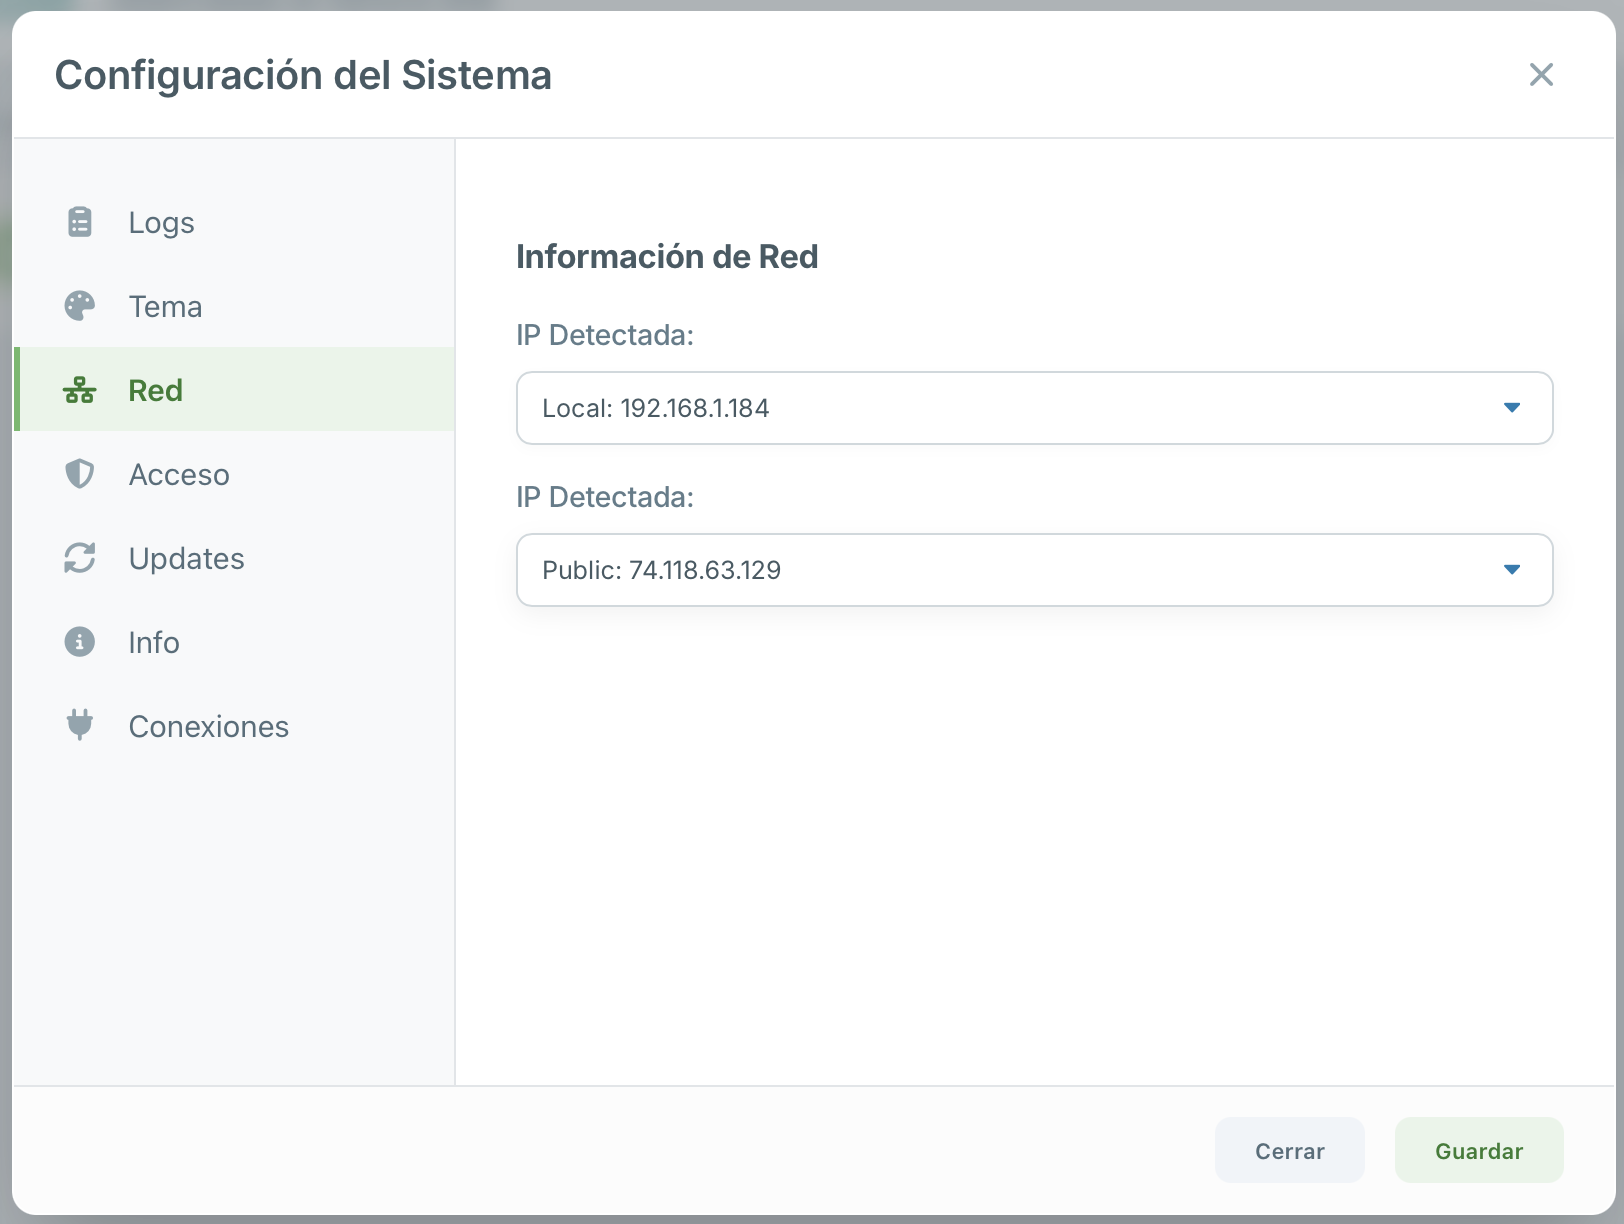
\includegraphics[width=0.95\textwidth]{anexos/18 red.png}
\caption{Configuracion avanzada de red}
\label{fig:red}
\end{figure}

\subsection{Parametros de Conexion}

\begin{table}[H]
\centering
\begin{tabular}{p{4.5cm}p{3cm}p{5.5cm}}
\toprule
\textbf{Parametro} & \textbf{Valor Default} & \textbf{Descripcion} \\
\midrule
Timeout de Conexion & 30 segundos & Tiempo maximo para establecer conexion \\
\midrule
Reintentos Automaticos & 3 intentos & Numero de reintentos ante fallo \\
\midrule
Intervalo de Keep-Alive & 60 segundos & Frecuencia de pings de mantenimiento \\
\midrule
Compresion de Datos & Activada & Reduce uso de ancho de banda \\
\midrule
Buffer de Red & 64 KB & Tamano del buffer de transmision \\
\bottomrule
\end{tabular}
\caption{Parametros configurables de red}
\label{tab:config-red}
\end{table}

\subsection{Configuracion de Proxy}

SDC soporta multiples configuraciones de proxy:

\begin{itemize}[leftmargin=*]
    \item \textbf{Proxy HTTP/HTTPS}: Configuracion estandar para trafico web
    \item \textbf{Proxy SOCKS5}: Para aplicaciones que requieren capa de transporte
    \item \textbf{Proxy Automatico (PAC)}: Deteccion automatica mediante script
    \item \textbf{Proxy por Aplicacion}: Cada app puede tener su propia configuracion
\end{itemize}

\subsection{Politicas de DNS}

\begin{quote}
\textbf{Resolucion DNS Segura}\\
SDC implementa DNS sobre HTTPS (DoH) y DNS sobre TLS (DoT) para prevenir ataques de envenenamiento de cache DNS y garantizar la privacidad de las consultas.
\end{quote}

\section{Control de Acceso}
\label{sec:acceso}

El sistema de control de acceso permite definir quien puede hacer que dentro de SDC.

\begin{figure}[H]
\centering
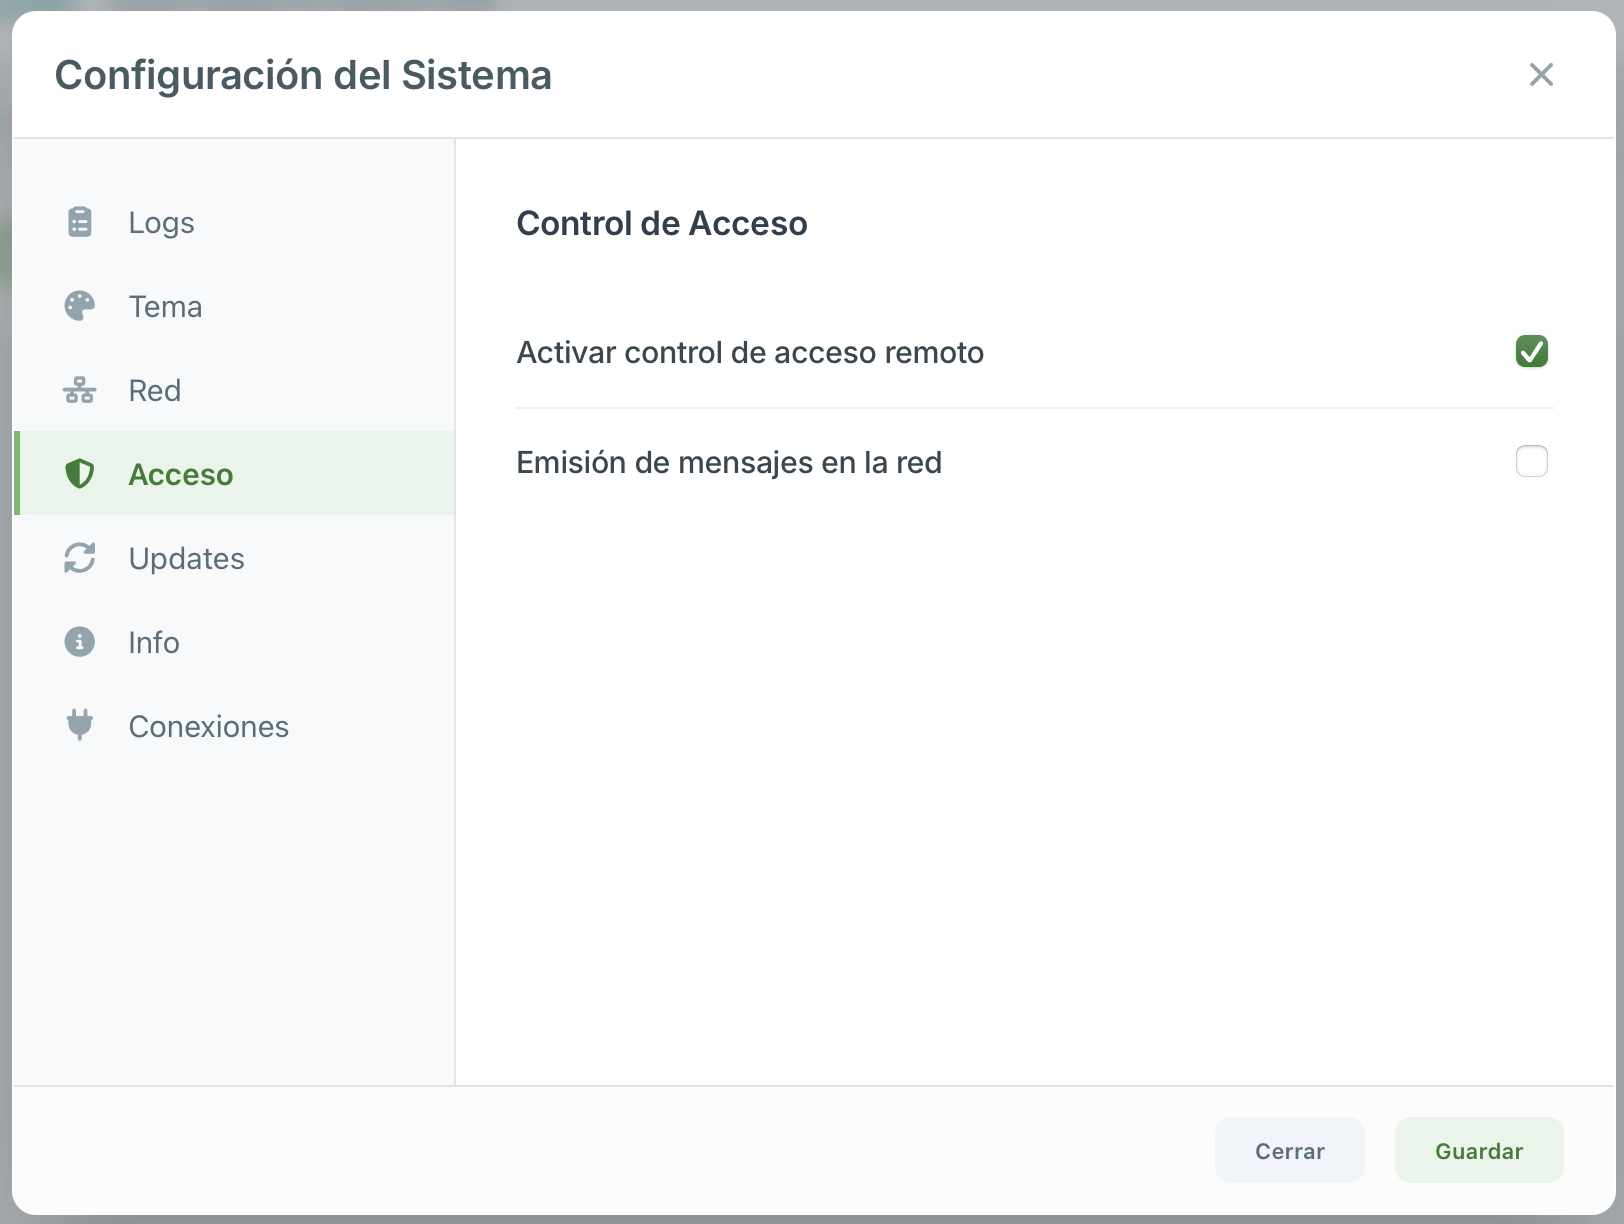
\includegraphics[width=0.95\textwidth]{anexos/19 acceso.png}
\caption{Panel de control de acceso}
\label{fig:acceso}
\end{figure}

\subsection{Niveles de Permisos}

\begin{table}[H]
\centering
\begin{tabular}{p{3cm}p{9.5cm}}
\toprule
\textbf{Nivel} & \textbf{Permisos} \\
\midrule
\textbf{Administrador} & Acceso total: configuracion del sistema, gestion de usuarios, auditoria completa, modificacion de politicas de seguridad \\
\midrule
\textbf{Operador} & Gestion de aplicaciones y conexiones, visualizacion de logs propios, uso de todas las herramientas excepto configuracion avanzada \\
\midrule
\textbf{Usuario} & Uso de aplicaciones asignadas, visualizacion de documentos autorizados, acceso limitado a metricas del sistema \\
\midrule
\textbf{Invitado} & Acceso temporal a aplicaciones publicas, sin capacidad de instalar o configurar \\
\bottomrule
\end{tabular}
\caption{Niveles de permisos de acceso}
\label{tab:niveles-acceso}
\end{table}

\subsection{Autenticacion Multifactor}

SDC soporta autenticacion adicional mediante:

\begin{itemize}[leftmargin=*]
    \item \textbf{Codigos TOTP}: Aplicaciones como Google Authenticator o Authy
    \item \textbf{Claves FIDO2/U2F}: Dispositivos fisicos como YubiKey
    \item \textbf{Biometria}: Huella dactilar o reconocimiento facial (segun hardware)
    \item \textbf{Tokens de Hardware}: Tarjetas inteligentes, certificados en USB
\end{itemize}

\section{Sistema de Actualizaciones}
\label{sec:updates}

El gestor de actualizaciones mantiene SDC al dia con las ultimas mejoras y parches de seguridad.

\begin{figure}[H]
\centering
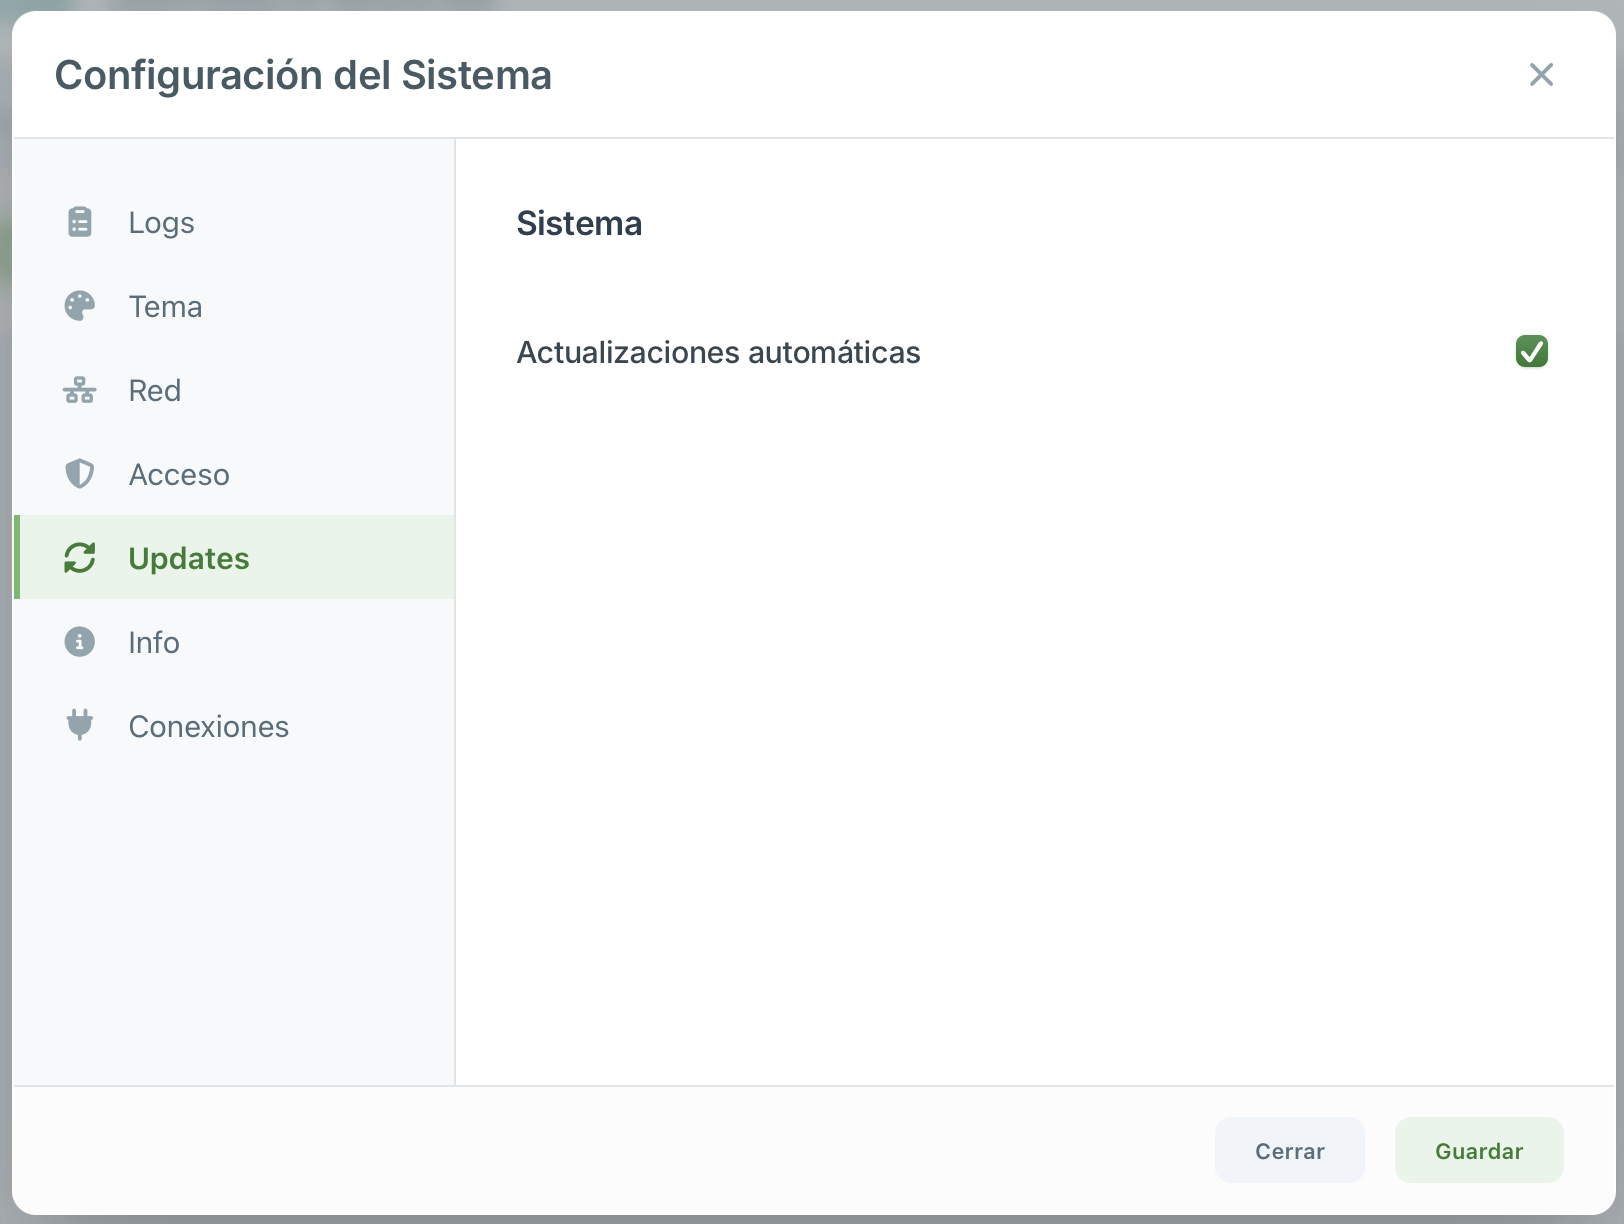
\includegraphics[width=0.95\textwidth]{anexos/20 updates.png}
\caption{Gestor de actualizaciones}
\label{fig:updates}
\end{figure}

\subsection{Canales de Actualizacion}

\begin{table}[H]
\centering
\begin{tabular}{p{3cm}p{4cm}p{5.5cm}}
\toprule
\textbf{Canal} & \textbf{Estabilidad} & \textbf{Recomendado Para} \\
\midrule
Stable & Alta & Entornos de produccion \\
\midrule
Beta & Media & Testing y desarrollo \\
\midrule
Nightly & Baja & Usuarios avanzados, QA \\
\midrule
LTS & Muy Alta & Sistemas criticos, compliance \\
\bottomrule
\end{tabular}
\caption{Canales de actualizacion disponibles}
\label{tab:canales-updates}
\end{table}

\subsection{Tipos de Actualizacion}

\begin{itemize}[leftmargin=*]
    \item \textbf{Actualizaciones de Seguridad}: Parches criticos (instalacion automatica recomendada)
    \item \textbf{Actualizaciones de Funciones}: Nuevas capacidades (instalacion manual)
    \item \textbf{Actualizaciones de Aplicaciones}: Nueva version de apps desplegadas
    \item \textbf{Definiciones de Seguridad}: Firmas antivirus, listas de bloqueo (automatico)
\end{itemize}

\begin{quote}
\textbf{Rollback de Actualizaciones}\\
Si una actualizacion causa problemas, SDC permite revertir a la version anterior automaticamente mediante el sistema de instantaneas (snapshots). El proceso toma menos de 2 minutos.
\end{quote}

\section{Informacion del Sistema}
\label{sec:info}

El panel de informacion del sistema proporciona datos tecnicos detallados sobre la instalacion actual.

\begin{figure}[H]
\centering
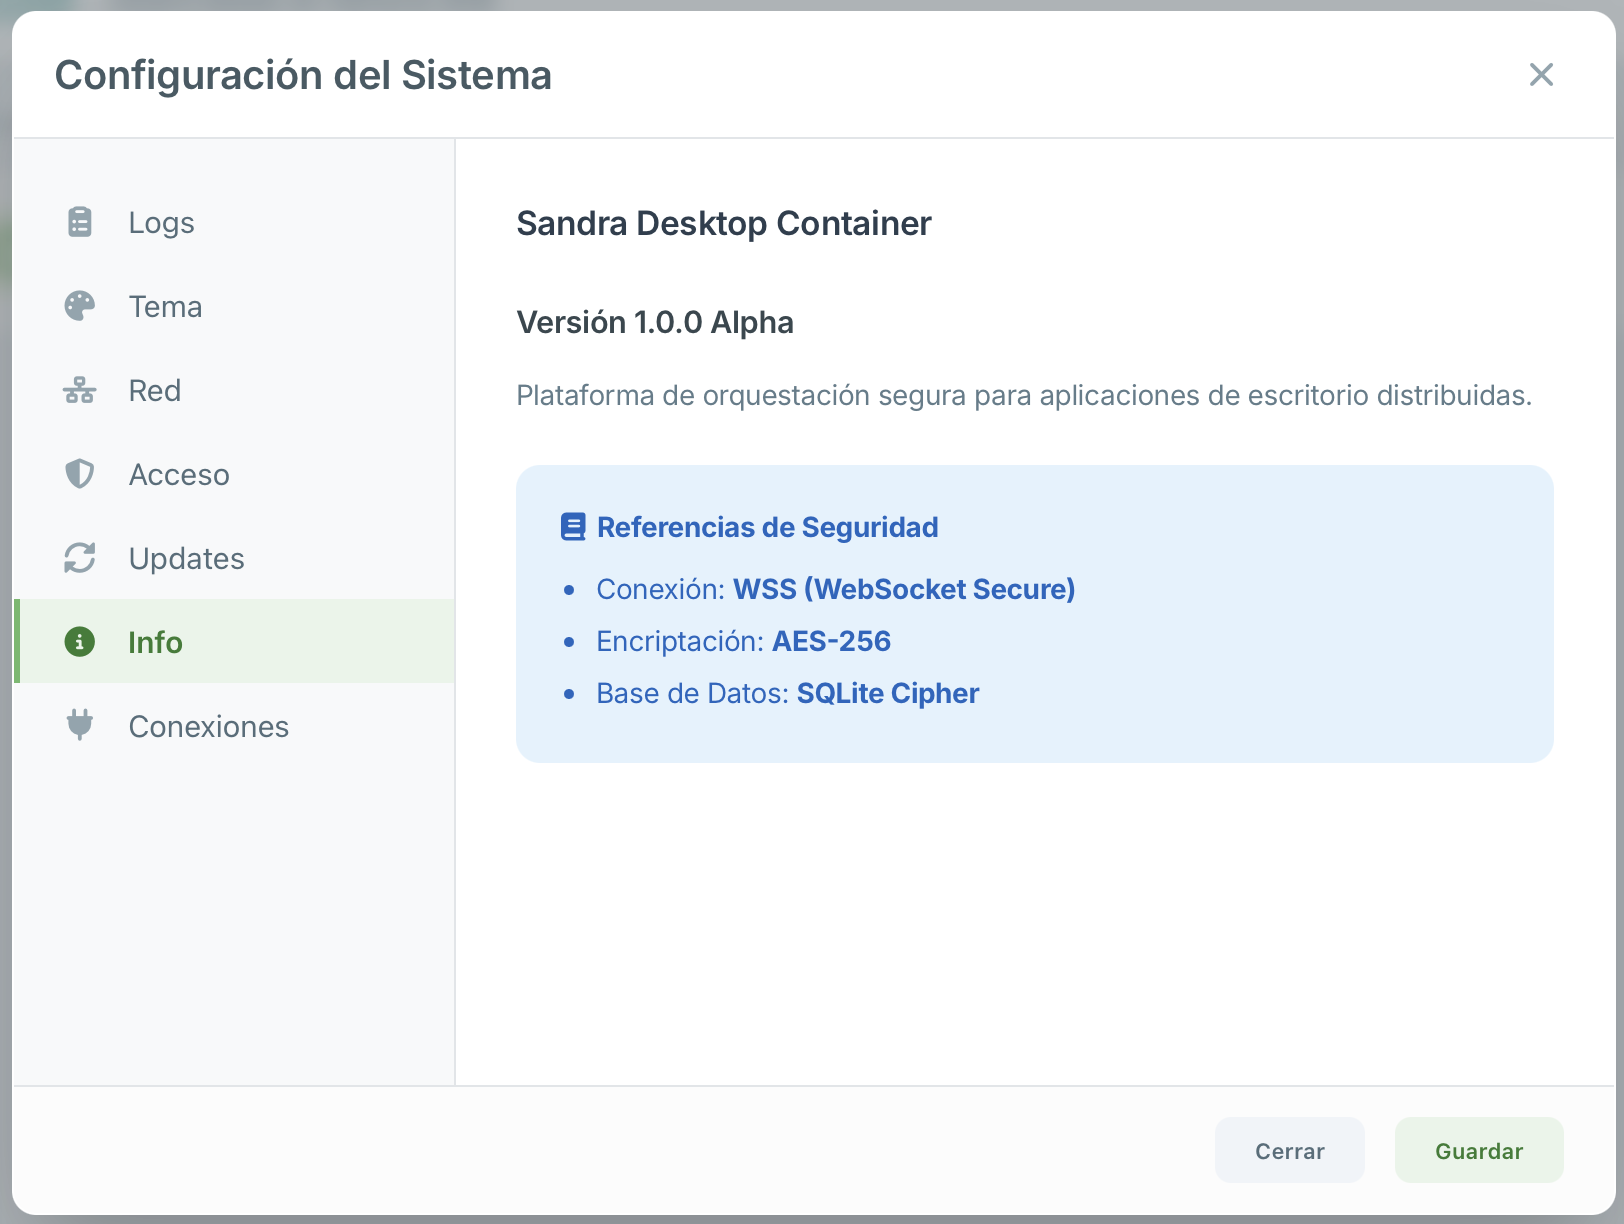
\includegraphics[width=0.95\textwidth]{anexos/21 info.png}
\caption{Informacion detallada del sistema}
\label{fig:info}
\end{figure}

\subsection{Datos Tecnicos Mostrados}

\begin{table}[H]
\centering
\begin{tabular}{p{4cm}p{9cm}}
\toprule
\textbf{Categoria} & \textbf{Informacion} \\
\midrule
\textbf{Version} & Numero de version de SDC, build date, commit hash \\
\midrule
\textbf{Runtime} & Version de Rust, Angular, Tauri, SQLite \\
\midrule
\textbf{Hardware} & CPU, RAM, almacenamiento, interfaces de red \\
\midrule
\textbf{Licencia} & Tipo de licencia, fecha de expiracion, caracteristicas habilitadas \\
\midrule
\textbf{Registro} & Client ID, fecha de instalacion, ultimo acceso \\
\bottomrule
\end{tabular}
\caption{Datos tecnicos del sistema}
\label{tab:datos-sistema}
\end{table}

\subsection{Exportacion de Diagnostico}

Para soporte tecnico, SDC puede generar un paquete de diagnostico que incluye:

\begin{itemize}[leftmargin=*]
    \item Logs del sistema (sin datos sensibles)
    \item Configuracion actual (anonimizada)
    \item Estado de componentes
    \item Historial de errores recientes
    \item Metricas de rendimiento
\end{itemize}

\begin{quote}
\textbf{Privacidad del Diagnostico}\\
Antes de generar el paquete de diagnostico, SDC permite revisar y excluir informacion que pueda considerarse sensible. Nunca se incluyen contrasenas, claves privadas o contenido de documentos.
\end{quote}

\section{Cierre del Sistema}
\label{sec:cierre}

El cierre seguro de SDC garantiza que todos los datos sensibles se protejan adecuadamente.

\begin{figure}[H]
\centering
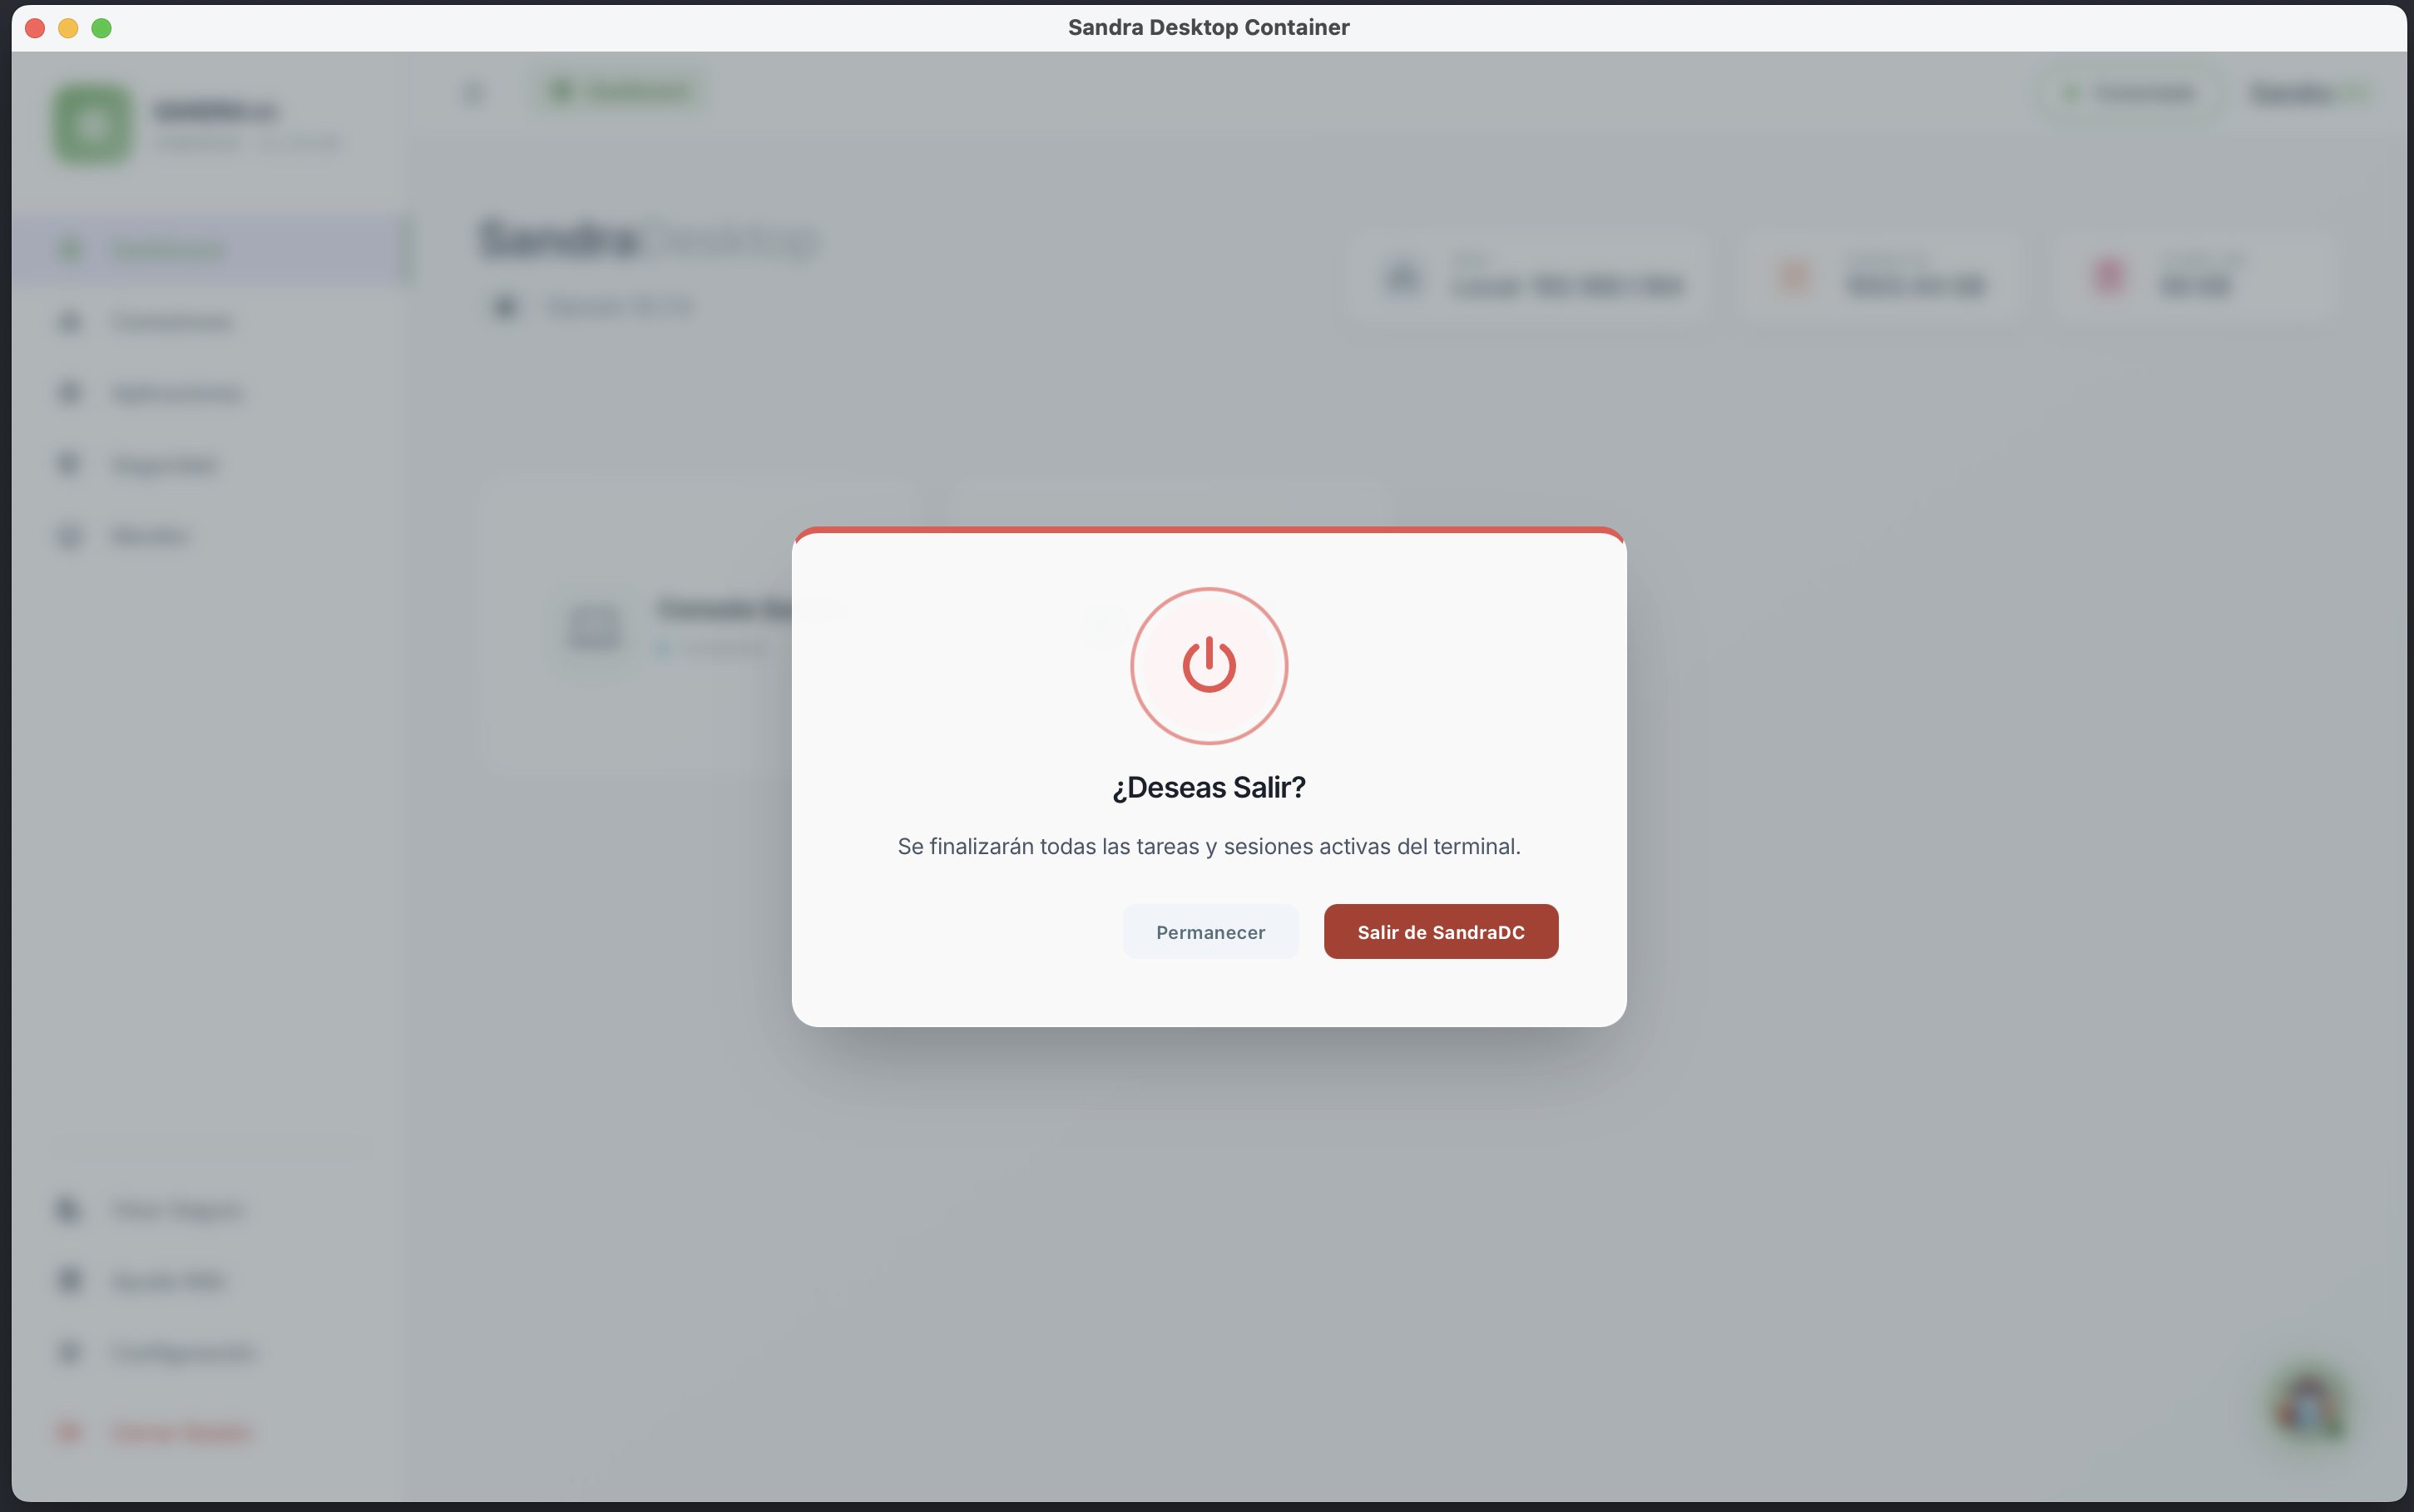
\includegraphics[width=0.95\textwidth]{anexos/fin sistema.png}
\caption{Pantalla de cierre del sistema}
\label{fig:cierre}
\end{figure}

\subsection{Procedimiento de Cierre}

Al cerrar SDC, el sistema realiza automaticamente:

\begin{enumerate}[leftmargin=*]
    \item \textbf{Limpieza de Memoria}: Todos los buffers de documentos abiertos se sobreescriben con ceros
    \item \textbf{Cierre de Conexiones}: Las conexiones activas se cierran ordenadamente
    \item \textbf{Persistencia de Estado}: La configuracion y preferencias se guardan en la base de datos
    \item \textbf{Bloqueo de Sesion}: El Client ID se marca como inactivo hasta el proximo inicio
    \item \textbf{Registro de Auditoria}: Se registra el evento de cierre con timestamp y duracion de la sesion
\end{enumerate}

\subsection{Opciones de Cierre}

\begin{table}[H]
\centering
\begin{tabular}{p{4cm}p{8.5cm}}
\toprule
\textbf{Opcion} & \textbf{Descripcion} \\
\midrule
Cierre Normal & Cierra aplicaciones de forma ordenada, guarda todo \\
\midrule
Cierre Rapido & Fuerza cierre inmediato, riesgo minimo de perdida de datos \\
\midrule
Cierre y Bloqueo & Cierra SDC y bloquea la pantalla del sistema \\
\midrule
Cierre y Suspender & Cierra SDC y suspende el dispositivo \\
\bottomrule
\end{tabular}
\caption{Opciones de cierre disponibles}
\label{tab:opciones-cierre}
\end{table}

\begin{quote}
\textbf{Advertencia Importante}\\
Evita cerrar SDC forzosamente (matar el proceso) mientras tengas documentos sensibles abiertos en el visor. Esto podria comprometer la garantia de zero-fill de la memoria. Siempre usa el cierre ordenado mediante el menu o el boton de cierre seguro.
\end{quote}

\section{Mejores Practicas de Configuracion}

\begin{enumerate}[leftmargin=*]
    \item \textbf{Realiza Backups}: Exporta tu configuracion periodicamente antes de cambios mayores
    \item \textbf{Documenta Cambios}: Manten un registro de modificaciones para auditoria
    \item \textbf{Prueba en Desarrollo}: Valida configuraciones nuevas en entorno de pruebas primero
    \item \textbf{Revisa Actualizaciones}: Lee las notas de release antes de actualizar
    \item \textbf{Configura Alertas}: Activa notificaciones para eventos criticos del sistema
\end{enumerate}


%--------------------------------------------------------------------
% ANEXOS
%--------------------------------------------------------------------
\appendix
\part{Anexos Técnicos}
%======================================================================
% ANEXOS TECNICOS - SANDRA DESKTOP CONTAINER
%======================================================================

\chapter{Anexos Tecnicos}
\label{ch:anexos}

Este apendice contiene informacion tecnica detallada sobre la arquitectura, flujos de datos y referencias de \textbf{Sandra Desktop Container}.

\section{Arquitectura de Software SDC}
\label{sec:arquitectura}

La arquitectura de SDC esta organizada en capas:

\begin{table}[H]
\centering
\begin{tabular}{p{4cm}p{5cm}p{5cm}}
\toprule
\textbf{Capa} & \textbf{Componentes} & \textbf{Tecnologia} \\
\midrule
Presentacion & Angular UI, Signals, SDC Services & Angular 15+ \\
\midrule
Puente & IPC Bridge, Commands API, Events API & Tauri 2.0 \\
\midrule
Core & Crypto, SQLite, WebSocket, Sandbox & Rust + Tokio \\
\midrule
Sistema & File System, Network, Process Mgmt & OS Nativo \\
\bottomrule
\end{tabular}
\caption{Arquitectura multicapa de SDC}
\label{tab:arquitectura-sdc}
\end{table}

\section{Ciclo de Vida de un Contenedor}
\label{sec:ciclo-vida}

Los contenedores en SDC siguen una maquina de estados:

\begin{enumerate}
    \item \textbf{CREADO}: El contenedor ha sido configurado pero no iniciado
    \item \textbf{CONFIGURADO}: Parametros de ejecucion establecidos
    \item \textbf{EJECUTANDO}: El contenedor esta activo y procesando
    \item \textbf{PAUSADO}: Ejecucion temporalmente detenida
    \item \textbf{DETENIDO}: Ejecucion finalizada, recursos liberados
    \item \textbf{DESTRUIDO}: Contenedor eliminado permanentemente
\end{enumerate}

\section{Flujo de Cifrado de Datos}
\label{sec:flujo-cifrado}

El proceso de cifrado en SDC:

\begin{enumerate}
    \item \textbf{Datos en Texto Plano} ingresan al sistema
    \item \textbf{Generacion de Clave}: Se crea una clave AES-256 unica
    \item \textbf{Derivacion HKDF}: La clave se procesa mediante HKDF-SHA256
    \item \textbf{Hash Argon2id}: Se aplica Argon2id para fortalecer la clave
    \item \textbf{Cifrado AES-256-GCM}: Los datos se cifran con autenticacion
    \item \textbf{Nonce}: Se genera un nonce de 96 bits unico por operacion
    \item \textbf{Almacenamiento}: Datos cifrados persistidos de forma segura
\end{enumerate}

\section{Topologia de Red}
\label{sec:topologia-red}

\begin{table}[H]
\centering
\begin{tabular}{p{4cm}p{4cm}p{5cm}}
\toprule
\textbf{Componente} & \textbf{Conexion} & \textbf{Protocolo} \\
\midrule
Nodos Cliente (SDC) & Internet & TLS 1.3 \\
\midrule
Servidor Principal & Internet & WSS (Puerto 8443) \\
\midrule
Servidor Replica & Internet & WSS (Puerto 8443) \\
\midrule
Base de Datos & Servidores & AES-256 \\
\bottomrule
\end{tabular}
\caption{Topologia de red del ecosistema SDC}
\label{tab:topologia-red}
\end{table}

\section{Tablas de Referencia Rapida}
\label{sec:tablas-ref}

\subsection{Puertos y Protocolos}

\begin{table}[H]
\centering
\begin{tabular}{p{2cm}p{3cm}p{4cm}p{4cm}}
\toprule
\textbf{Puerto} & \textbf{Protocolo} & \textbf{Uso} & \textbf{Seguridad} \\
\midrule
8443 & WSS & Comunicacion cliente-servidor & TLS 1.3 + Client Auth \\
\midrule
8080 & WS & Desarrollo local & Sin cifrado \\
\midrule
443 & HTTPS & API REST & TLS 1.3 \\
\midrule
3000 & HTTP & Desarrollo Angular & Solo localhost \\
\bottomrule
\end{tabular}
\caption{Puertos y protocolos utilizados por SDC}
\label{tab:puertos}
\end{table}

\subsection{Algoritmos Criptograficos}

\begin{table}[H]
\centering
\begin{tabular}{p{4cm}p{4cm}p{5cm}}
\toprule
\textbf{Proposito} & \textbf{Algoritmo} & \textbf{Parametros} \\
\midrule
Cifrado Simetrico & AES-256-GCM & Clave: 256 bits, Nonce: 96 bits \\
\midrule
Hashing de Contrasenas & Argon2id & Memoria: 64MB, Iteraciones: 3 \\
\midrule
Derivacion de Claves & HKDF-SHA256 & Salt: 128 bits \\
\midrule
Cifrado Asimetrico & RSA-4096 & OAEP padding, SHA-256 \\
\midrule
Firma Digital & ECDSA P-256 & Curva secp256r1 \\
\bottomrule
\end{tabular}
\caption{Algoritmos criptograficos implementados}
\label{tab:crypto}
\end{table}

\subsection{Codigos de Error}

\begin{table}[H]
\centering
\begin{tabular}{p{3cm}p{4cm}p{6cm}}
\toprule
\textbf{Codigo} & \textbf{Descripcion} & \textbf{Accion Recomendada} \\
\midrule
SDC-E001 & Fallo de autenticacion & Verificar credenciales y Client ID \\
\midrule
SDC-E002 & Conexion rechazada & Verificar red y estado del servidor \\
\midrule
SDC-E003 & Certificado invalido & Actualizar certificados CA del sistema \\
\midrule
SDC-E004 & Timeout agotado & Aumentar timeout o verificar latencia \\
\midrule
SDC-E005 & Violacion de seguridad & Contactar administrador inmediatamente \\
\midrule
SDC-E006 & Espacio insuficiente & Liberar espacio en disco \\
\midrule
SDC-E007 & Formato no soportado & Verificar compatibilidad del archivo \\
\midrule
SDC-E008 & Sesion expirada & Reiniciar sesion de autenticacion \\
\bottomrule
\end{tabular}
\caption{Codigos de error estandar de SDC}
\label{tab:errores}
\end{table}

\section{Glosario de Terminos Tecnicos Extendido}
\label{sec:glosario-tecnico}

\begin{description}[leftmargin=*, style=nextline]
    \item[\textbf{AES-256-GCM}] Advanced Encryption Standard con clave de 256 bits en modo Galois/Counter Mode. Proporciona cifrado autenticado.
    
    \item[\textbf{Argon2id}] Variante del algoritmo Argon2 disenada para resistir ataques de canal lateral y GPU.
    
    \item[\textbf{Client ID}] Identificador unico criptografico asignado a cada nodo SDC.
    
    \item[\textbf{Defensa en Profundidad}] Estrategia de seguridad que implementa multiples capas de proteccion.
    
    \item[\textbf{HKDF}] HMAC-based Key Derivation Function. Algoritmo para derivar multiples claves criptograficas.
    
    \item[\textbf{IPC}] Inter-Process Communication. Mecanismo de comunicacion entre Angular y Rust.
    
    \item[\textbf{Ruta Proxy}] Punto de acceso configurado que actua como intermediario seguro.
    
    \item[\textbf{Sandbox}] Entorno de ejecucion aislado donde las micro-aplicaciones operan.
    
    \item[\textbf{SID}] Secure ID. Identificador unico trazable asignado a cada operacion.
    
    \item[\textbf{WSS}] WebSocket Secure. Protocolo de comunicacion bidireccional sobre TLS.
\end{description}


%--------------------------------------------------------------------
% FIN
%--------------------------------------------------------------------
\backmatter
\printindex

\end{document}
